
\section*{Learning Objectives}By completing this chapter, students will:

\begin{itemize}
\item Gain an introduction to differential equations, focusing on their significance and the various classifications.
\item Learn the foundational theories and techniques for solving one-dimensional first-order ordinary differential equations (ODEs).
\item Acquire knowledge on the fundamentals and solution methods for vector first-order ODEs.
\item Explore the application of numerical methods in solving vector first-order ODEs.
\item Delve into the characteristics of linear systems of first-order ODEs and their implications for mathematical modeling.
\end{itemize}

\section*{Outcomes}
Upon mastering the content of this chapter, students will be equipped to:

\begin{itemize}
\item Understand the definition and classification of ODEs based on their order, linearity, and whether they are homogeneous or non-homogeneous.
\item Engage with various strategies for tackling first-order ODEs, covering separable, linear, and select nonlinear equations.
\item Dive into the theory and application of solving systems of linear differential equations, highlighting their importance across diverse applications.
\item Comprehend the utilization of ODEs in modeling and solving real-world problems across various domains.
\item Grasp the fundamentals of numerical methods designed for solving ODEs in scenarios where analytic solutions are challenging or unattainable.
\item Deeply investigate linear systems of ODEs, focusing on:
    \begin{itemize}
    \item The structure and solution of linear vector ODEs, symbolized as $\dot{x} = Ax, x(t_0) = x_0$.
    \item The concept and significance of the matrix exponential, denoted as $e^{At}$.
    \item Essential attributes of the matrix exponential, such as $\frac{d}{dt} e^{At} = A e^{At} =  e^{At} A$.
    \item Methods for solving linear vector ODEs, exemplified by $x(t) = e^{A(t-t_0)} x_0$.
    \item The role of complex scalar exponentials,  $e^{\left( a + \im \omega \right) t}$,  in the context of ODE solutions.
    \item The interplay between eigenvectors, eigenvalues, and the matrix exponential, such as  $Av = \lambda v \implies  e^{A(t-t_0)} v = e^{\lambda(t-t_0)} v$.
    \item The criteria for stability in linear systems, ${\rm real} (\lambda) < 0 \implies \lim_{t\to \infty} e^{A(t-t_0)} v = 0_{n \times 1}$, underlining how the real parts of eigenvalues influence the system's long-term behavior.
    \item The application of these principles to general initial conditions when $A$ has a complete set of eigenvectors.        
    \end{itemize}    
\end{itemize}



% \newpage
% \section*{Learning Objectives}

% \begin{itemize}
%     \item To introduce the concept of differential equations and their classifications.
%     \item To understand the basic theory and methods of solving one-dimensional first-order ODEs.
%     \item To understand the basic theory and methods of solving vector first-order ODEs.
%     \item To understand numerical methods of solving vector first-order ODEs.
%     \item To understand the properties of linear systems of first-order ODEs.
% \end{itemize}

% \section*{Outcomes}
% \begin{itemize}
%     \item Understanding what constitutes an ODE and how they are classified based on order, linearity, and homogeneity.
%     \item Delving into methods of solving first-order ODEs, including separable equations, linear equations, and some nonlinear equations.
%     \item An introduction to solving systems of linear differential equations, which is crucial in many applications.
%     \item Understanding how ODEs are used to model and solve problems in various fields.
%     \item Introducing basic numerical methods for solving ODEs when analytical solutions are difficult or impossible to find.
%     \item A deep dive into linear systems of ODES:
%     \begin{itemize}
%     \item Linear vector ODEs, $\dot{x} = Ax, x(t_0) = x_0$
%     \item Matrix exponential, $e^{At}$
%     \item Key properties of the matrix exponential, such as $\frac{d}{dt} e^{At} = A e^{At} =  e^{At} A$
%     \item Solution of linear vector ODES, $x(t) = e^{A(t-t_0)} x_0$
%     \item Complex (scalar) exponentials, $e^{\left( a + \im \omega \right) t}$
%     \item Eigenvectors and eigenvalues of the matrix exponential, $Av = \lambda v \implies  e^{A(t-t_0)} v = e^{\lambda(t-t_0)} v$
%     \item ${\rm real} (\lambda) < 0 \implies \lim_{t\to \infty} e^{A(t-t_0)} v = 0_{n \times 1}$
%     \item Extension of the above to general initial conditions where there is a full set of e-vectors.         
%     \end{itemize}    
% \end{itemize}
% \newpage


\begin{figure}[htb]%
\centering
\subfloat[]{%
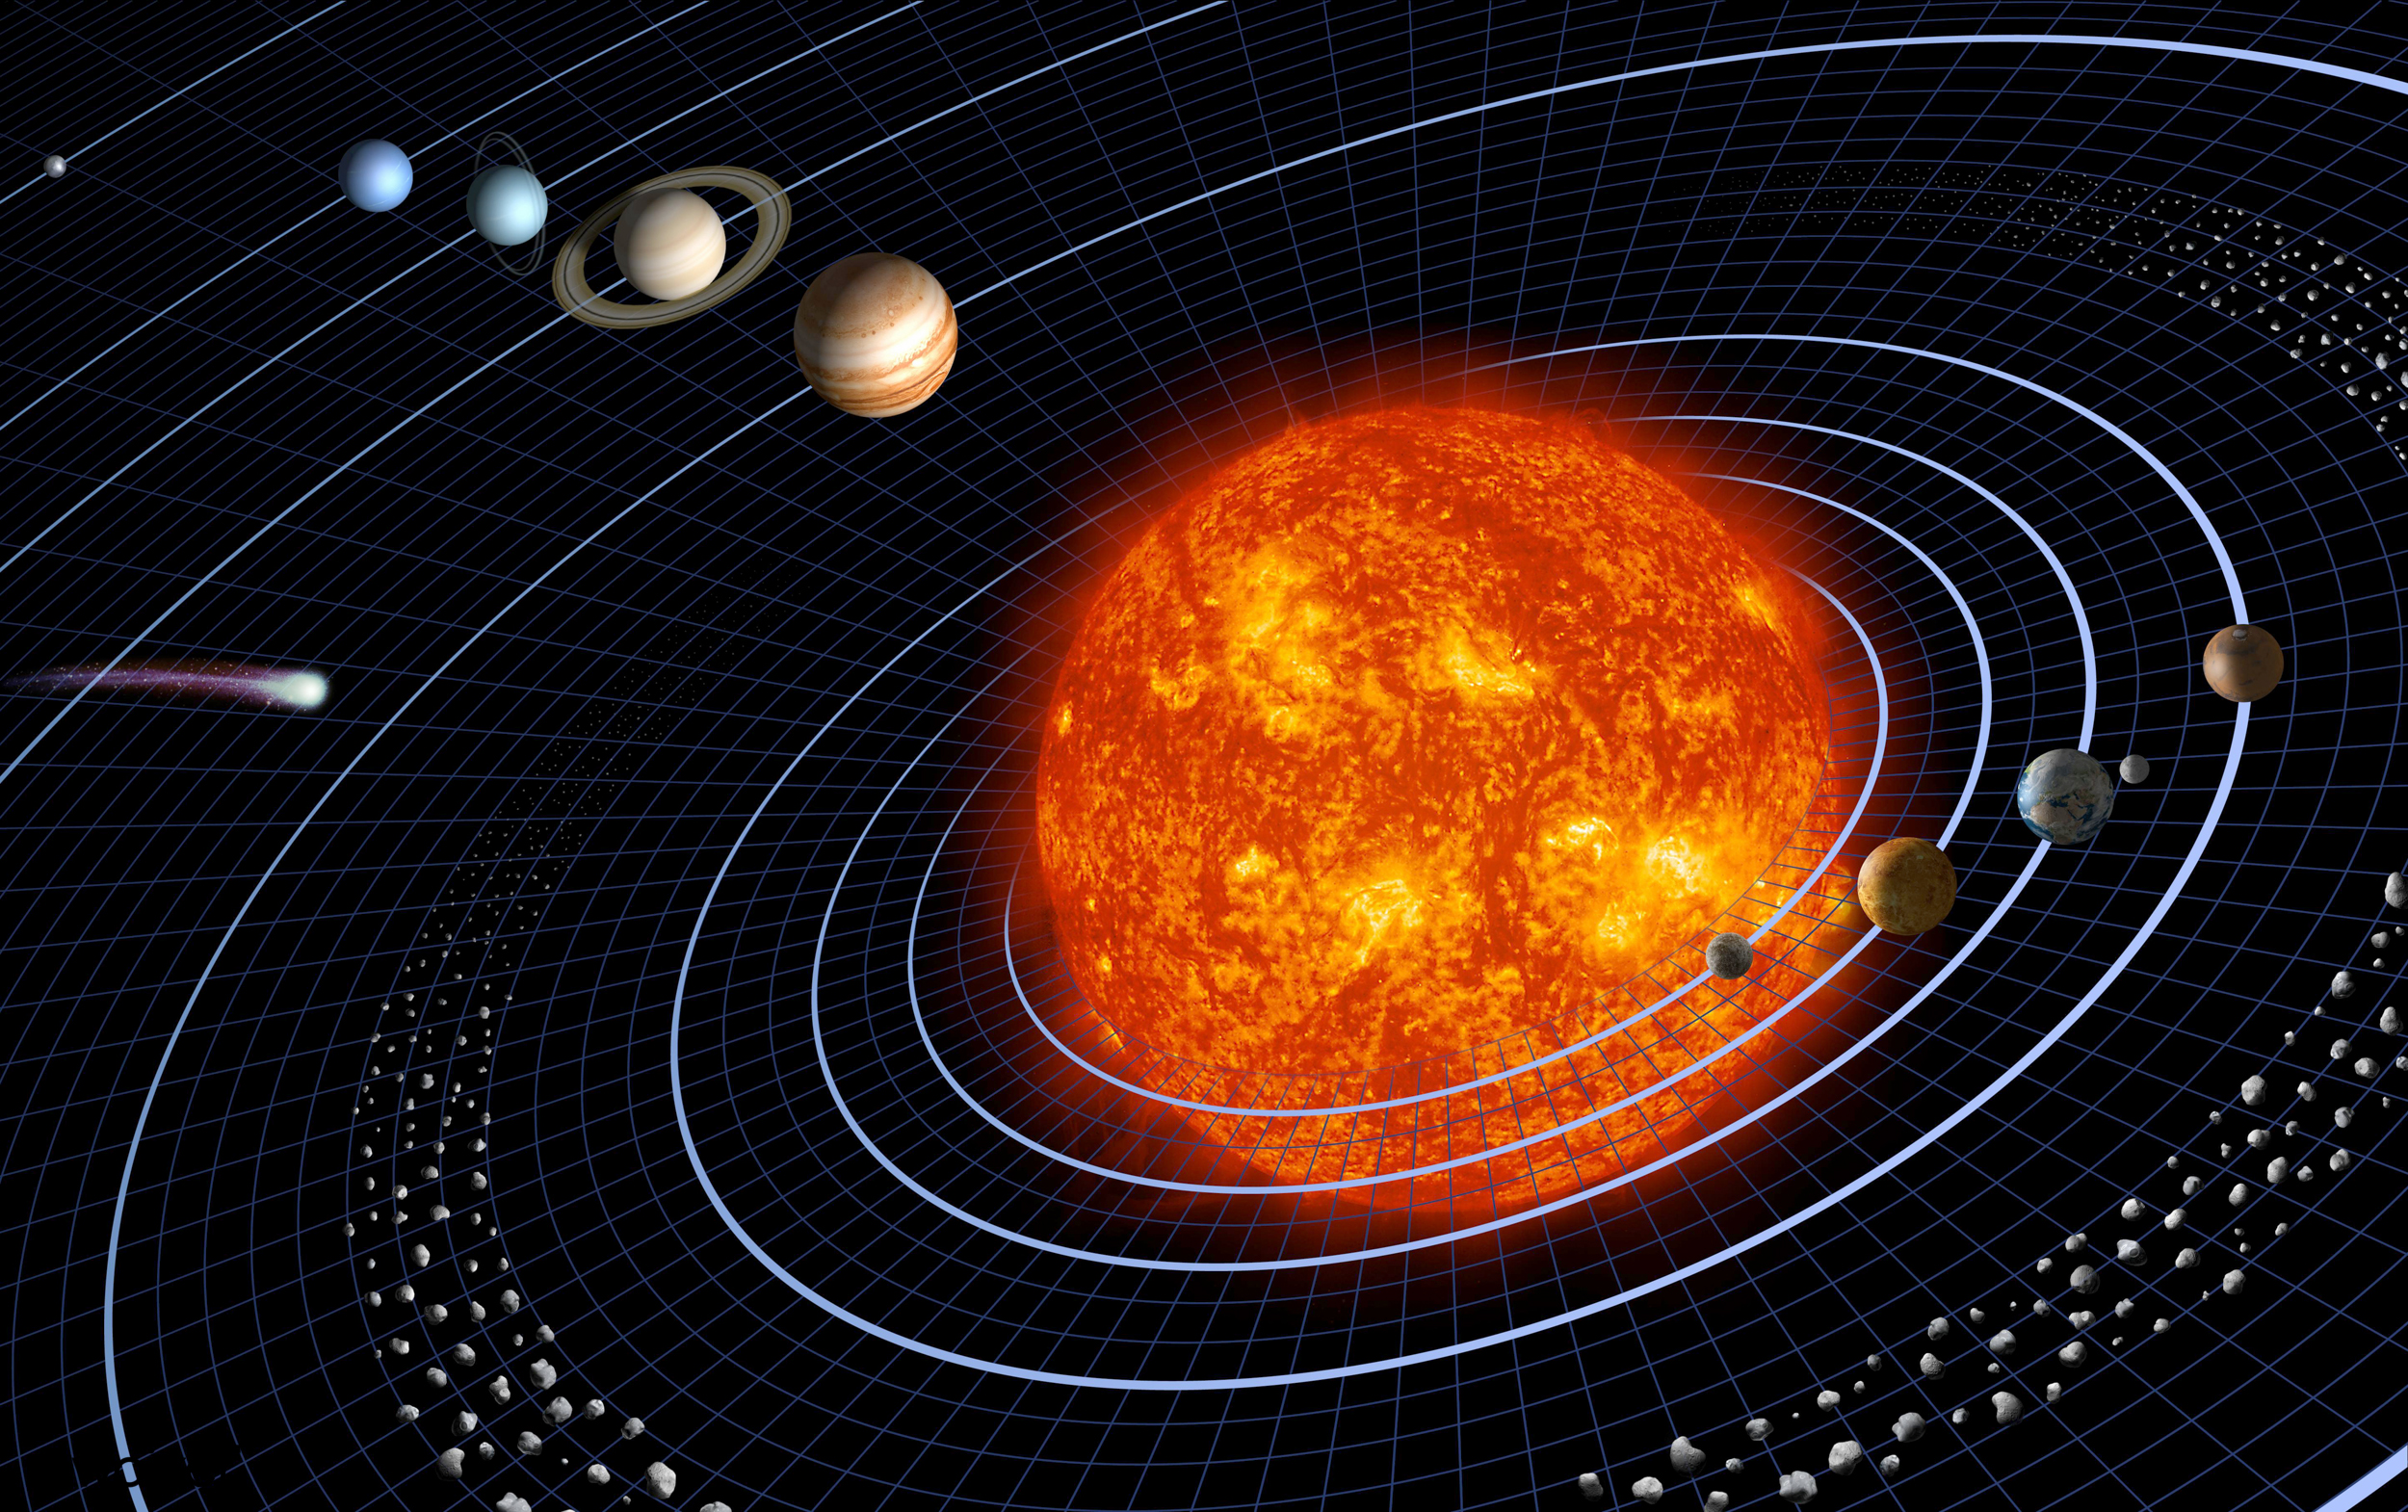
\includegraphics[height=0.39\columnwidth]{graphics/Chap09/EarthSolarSystemWorldHistoryEncyclopedia.jpg}}%
\hfill%
\subfloat[]{%
%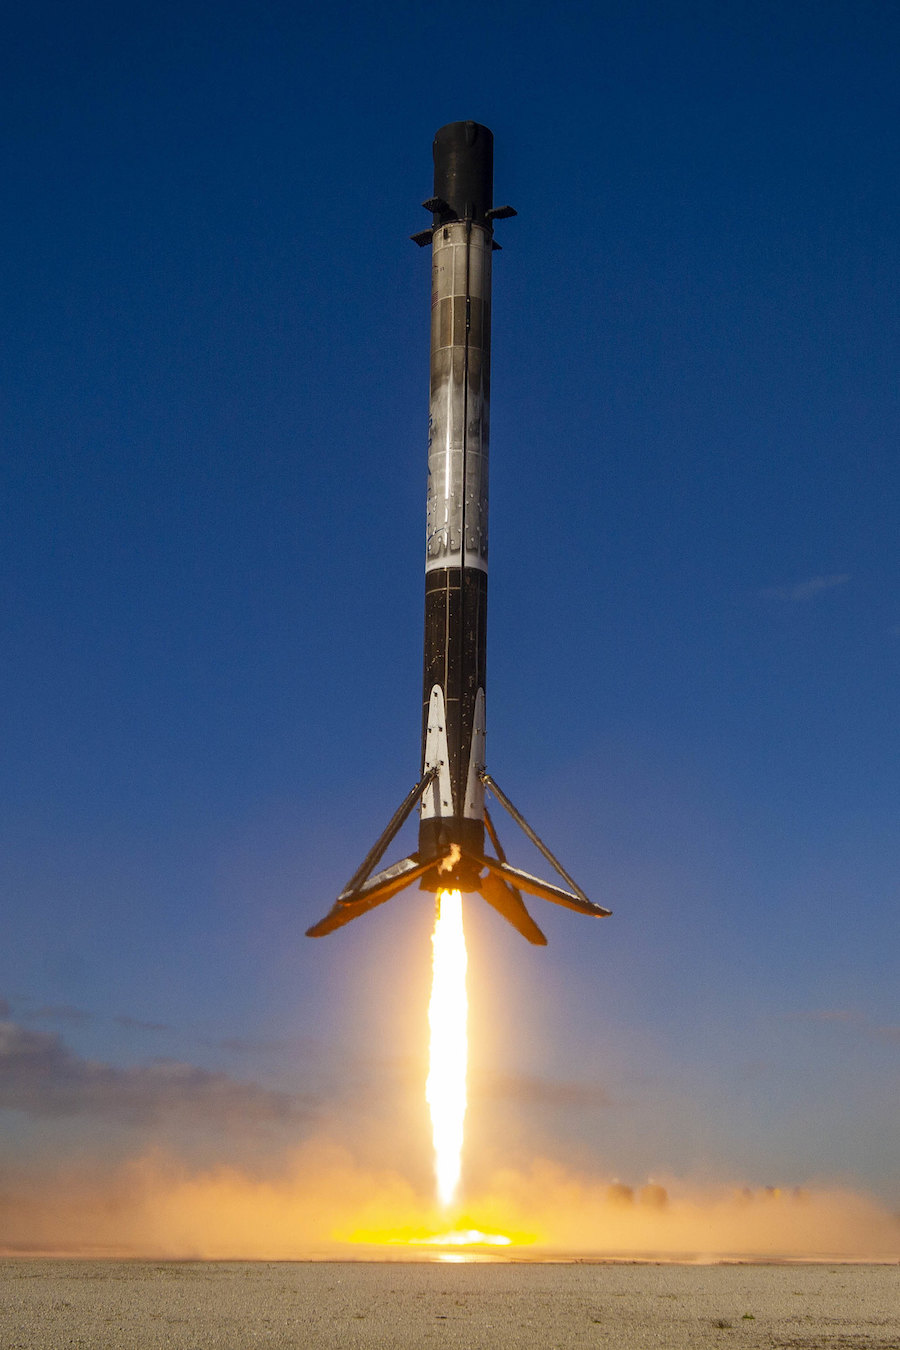
\includegraphics[trim=10 10 10 10, clip, height=0.37\columnwidth]{graphics/Chap09/SpaceXBoosterStageLanding.jpg} %%% left2 bottom2 right2 top2
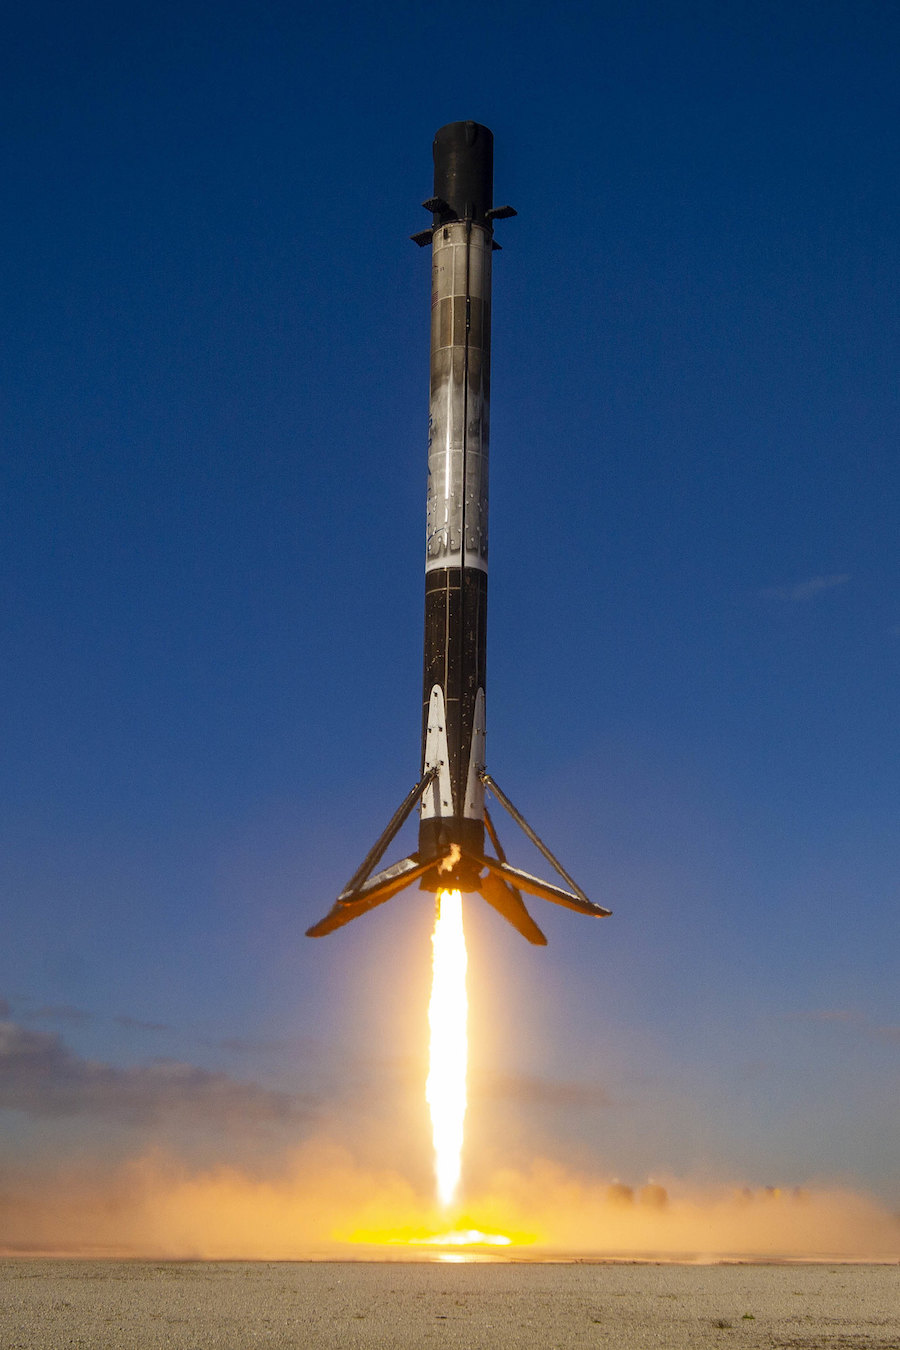
\includegraphics[trim=100 0 100 0, clip, height=0.39\columnwidth]{graphics/Chap09/SpaceXBoosterStageLanding.jpg}}%
\hfill%
\subfloat[]{%
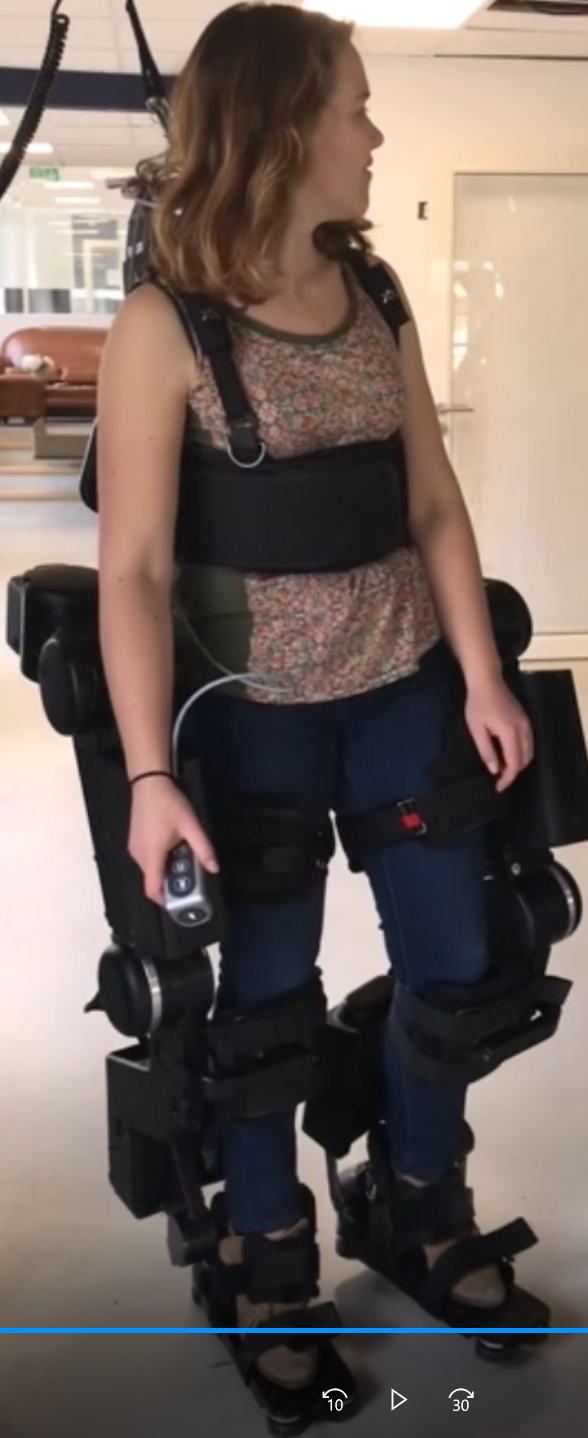
\includegraphics[height=0.39\columnwidth]{graphics/Chap09/WandercraftMarineExo2022.png}}%
\hfill
    \caption[]{\textbf{What do we have in common?} (a) Illustration of the solar system. (b) Space-X landing a booster. (c) Wandercraft's exoskeleton allows patients with paraplegia (paralysis from the waist down) to walk again. Sources: (a) \href{https://www.worldhistory.org/image/11979/earths-solar-system/}{World History Encyclopedia} (b) \href{https://spaceflightnow.com/2021/06/28/spacex-launch-this-week-will-feature-first-onshore-rocket-landing-since-december/}{SpaceX-Booster} (c) \href{https://www.tf1info.fr/high-tech/exclusif-wandercraft-fait-remarcher-les-paraplegiques-2113727.html}{TF1 Info: Wandercraft fait remarcher les parapl\'egiques gr\^ace \`a un exosquelette}}
    \label{fig:WhatDoWeHaveInCommon}
\end{figure}

\section{Introduction}

Figure~\ref{fig:WhatDoWeHaveInCommon} illustrates three ``objects'' where \textbf{ordinary differential equations (ODEs)} are required to understand how they function. A differential equation is an equation that includes one or more derivatives, such as
$$
\begin{aligned}
    \dot{x}(t) + x(t) -\sin(t) = 0, ~~\text{or}\\
    \ddot{x}(t) + \dot{x}(t) + \left(x(t) +1 \right)^3 =0;
\end{aligned}
$$
if there were no derivatives, we could simply solve the equations for the unknown $x(t)$ and be done with it.
Got it. Then what makes an equation with derivatives ``ordinary''? It is an ``ordinary'' differential equation if the included derivatives are all with respect to the same scalar variable. If there are derivatives with respect to several variables (or a vector of variables), then they are called partial derivatives, and we would have a \href{https://youtu.be/ly4S0oi3Yz8}{partial differential equation}, or PDE for short. We've encountered a few ODEs already, in Example~\ref{ex:TotalDerivativeWithODE} dealing with the total derivative, and in Chapter~\ref{sec:LagrangianDynamics} on Lagrangian Dynamics, where we derived the equations of motion for a point mass in $\real^2$, a pendulum, a three-link manipulator, and a three-link bipedal walker. 

In the present Chapter, we explore what it means for a function (eventually, a vector of functions) to be a solution to an ODE. Similar to antiderivatives, we'll see that in some cases, a closed-form solution to an ODE can be found, while in other cases, the solution cannot be expressed in terms of simple functions and we rely on numerical methods for determining a solution.

\bigskip

\begin{funColor}{Understanding the Solar System has been a Major Driver of Scientific Inquiry}{SolarSystem}
The understanding of the solar system has evolved significantly over the centuries\footnote{\url{https://youtu.be/9xBoC26HBIw}{The day the universe changed 05 - James Burke}--starts off quite slow, but gets very interesting at 33 minutes, where you see Calculus thinking being employed 100 years before Calculus was formally invented by Newton and Leibniz.}. In the beginning, we humans postulated paths or orbits for the planets, such as perfect circles around the earth. Eventually, data showed that model was wrong, and it was replaced by ellipses around the sun. These early models were \textbf{descriptive}, meaning they described the observational data but did not attempt to explain the ``how'' or the ``why'' of the planets' orbits. \\

Newton proposed the first \textbf{mechanistic} model, with his famous law of gravitational attraction. It was eventually realized that Newton's laws were highly accurate for all of the planets except Mercury, which presented a significant puzzle to astronomers for many years. The issue was with its perihelion, the point in its orbit closest to the Sun. Over time, the perihelion of Mercury was observed to advance or shift in a way that couldn't be explained by Newtonian mechanics. \textit{Mercury's perihelion advanced by an additional 43 arcseconds per century more than what was predicted by Newton's laws}.\\

Mercury's orbital discrepancy was resolved by Albert Einstein's General Theory of Relativity in 1915, which is grounded in an advanced form of Calculus on surfaces. General Relativity describes gravity not as a force, but as a curvature of spacetime caused by mass. According to this theory, the path of a planet is a geodesic (a path of shortest distance, such as a great circle route on the earth) in the curved spacetime caused by the Sun. \\

\textbf{Timeline}
\begin{enumerate}
    \item \textbf{Geocentric Model (Ancient Times - 16th Century)}:  \textit{Ancient Greece (circa 4th century BCE)}: The geocentric model, with Earth at the center of the universe, was developed by Greek philosophers like Aristotle and later refined by Ptolemy (Egypt) in the 2nd century ACE.
        
    \item \textbf{Ptolemaic System (2nd century ACE)}: \textit{Claudius Ptolemy} detailed the geocentric model in his work ``Almagest,'' introducing epicycles to explain the retrograde motion of planets.

    \item \textbf{Nicolaus Copernicus (1543)}: \textit{Copernicus} proposed the heliocentric model in ``De revolutionibus orbium coelestium,'' suggesting that Earth and other planets revolve around the Sun.
        
    \item \textbf{Tycho Brahe (late 16th century)}: \textit{Brahe} proposed a hybrid model combining aspects of both geocentric and heliocentric theories.

 \item \textbf{Kepler's Laws of Planetary Motion (Early 17th Century)}: \textit{Johannes Kepler (1609 - 1619)}: Kepler formulated his three laws of planetary motion, describing elliptical orbits of planets around the Sun.
    
    \item \textbf{Newton's Law of Universal Gravitation (Late 17th Century)}: \textit{Isaac Newton (1687)}: In ``Principia Mathematica,'' Newton formulated the law of universal gravitation, explaining planetary motions and laying the groundwork for Newtonian physics.

    \item \textbf{Einstein's Theory of General Relativity (Early 20th Century)}: \textit{Albert Einstein (1915)}: Einstein's theory of general relativity further refined the understanding of gravitational forces and introduced the concept of spacetime curvature.

\end{enumerate}

   
\end{funColor}


\begin{figure}[htb]%
\centering
\subfloat[]{%
\hfill%
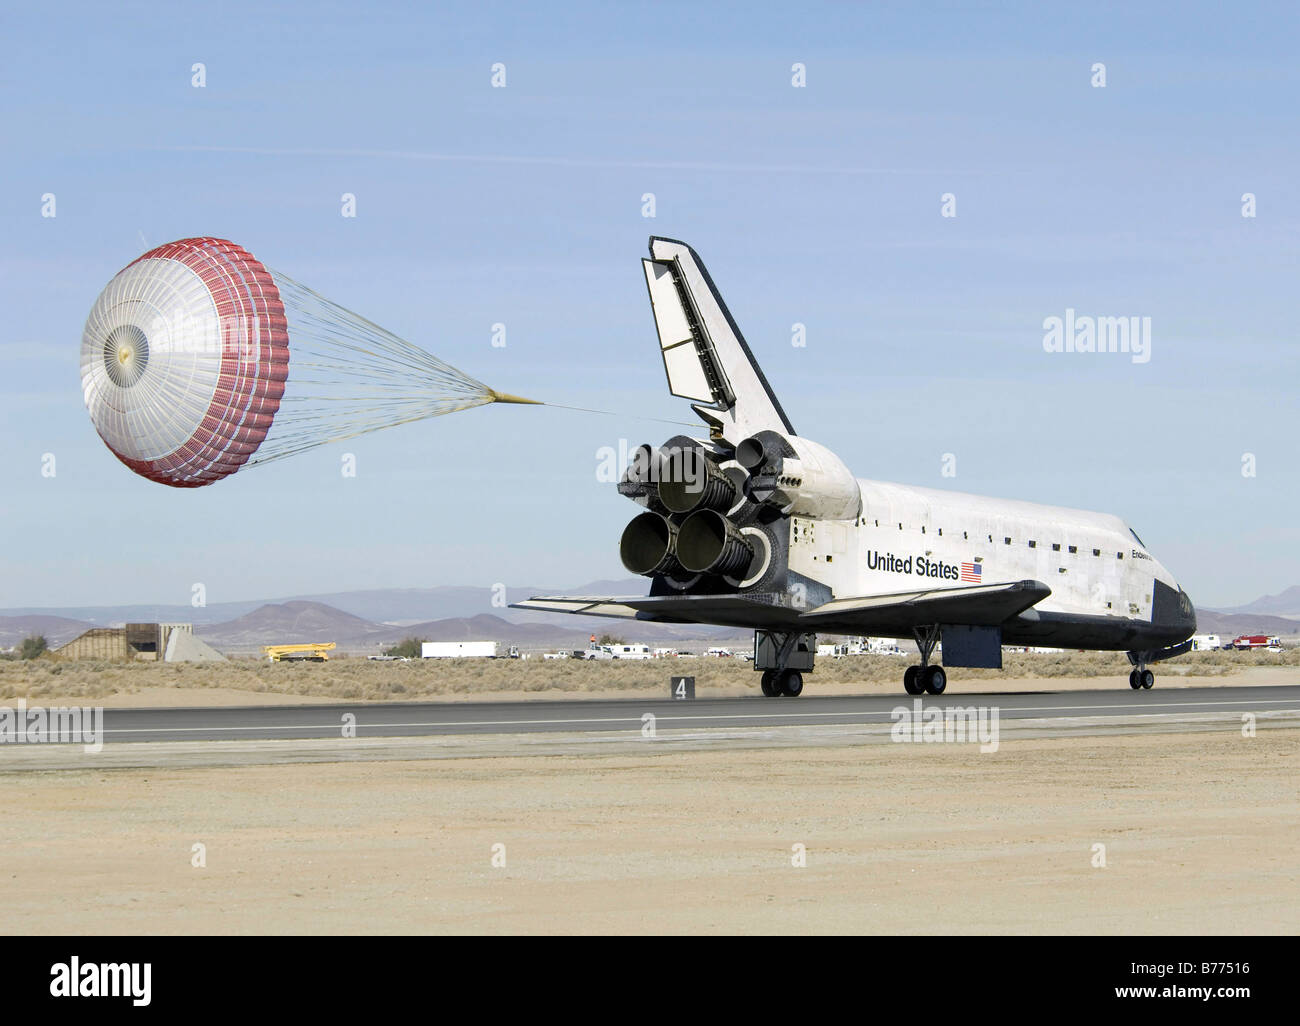
\includegraphics[height=0.39\columnwidth]{graphics/Chap09/space-shuttle-endeavour-with-its-drag-chute-deployed-B77516.jpg}}%
\hspace*{1cm}
\subfloat[]{%
%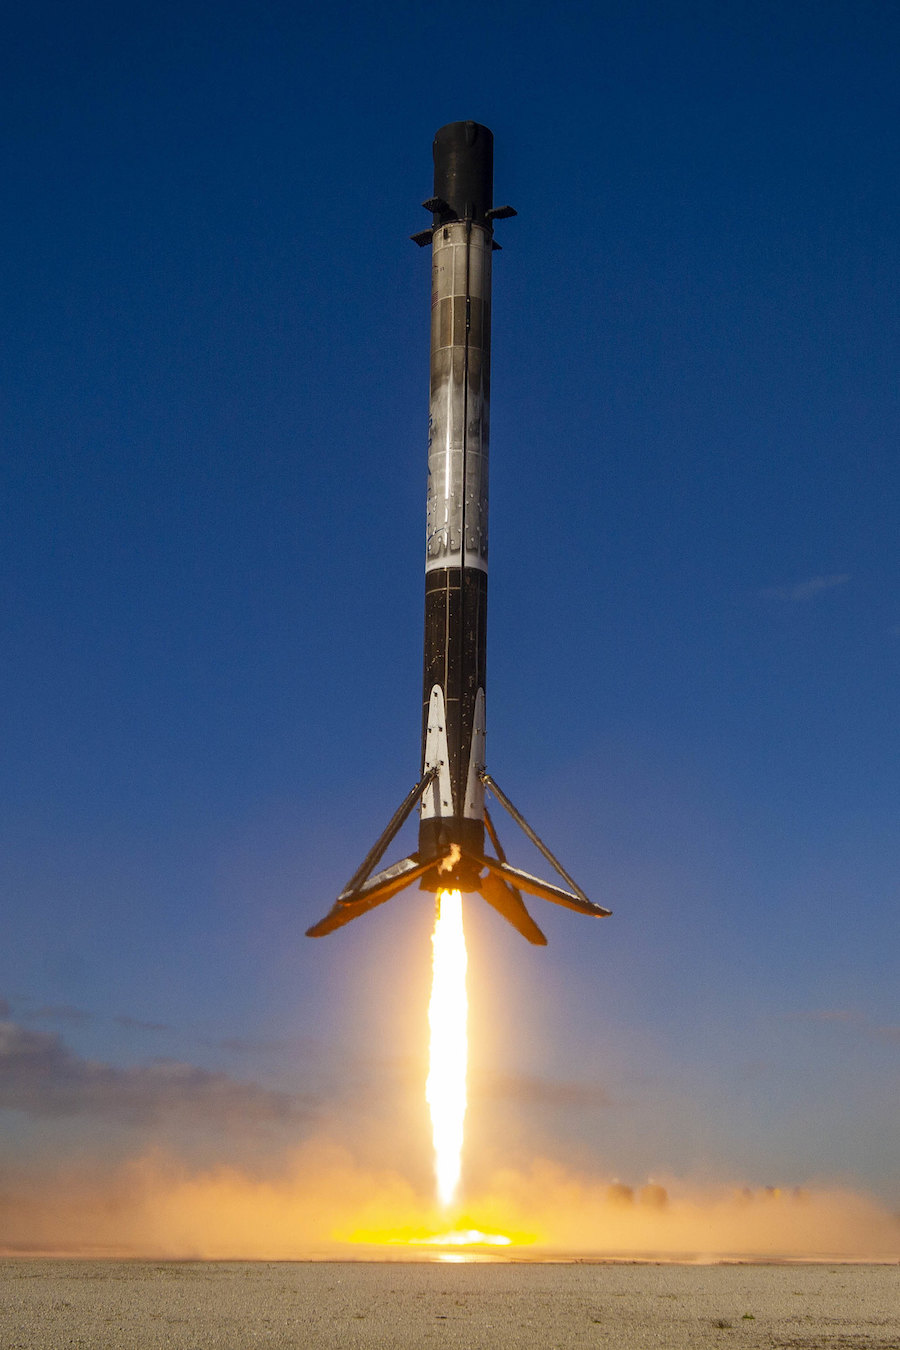
\includegraphics[trim=10 10 10 10, clip, height=0.37\columnwidth]{graphics/Chap09/SpaceXBoosterStageLanding.jpg} %%% left2 bottom2 right2 top2
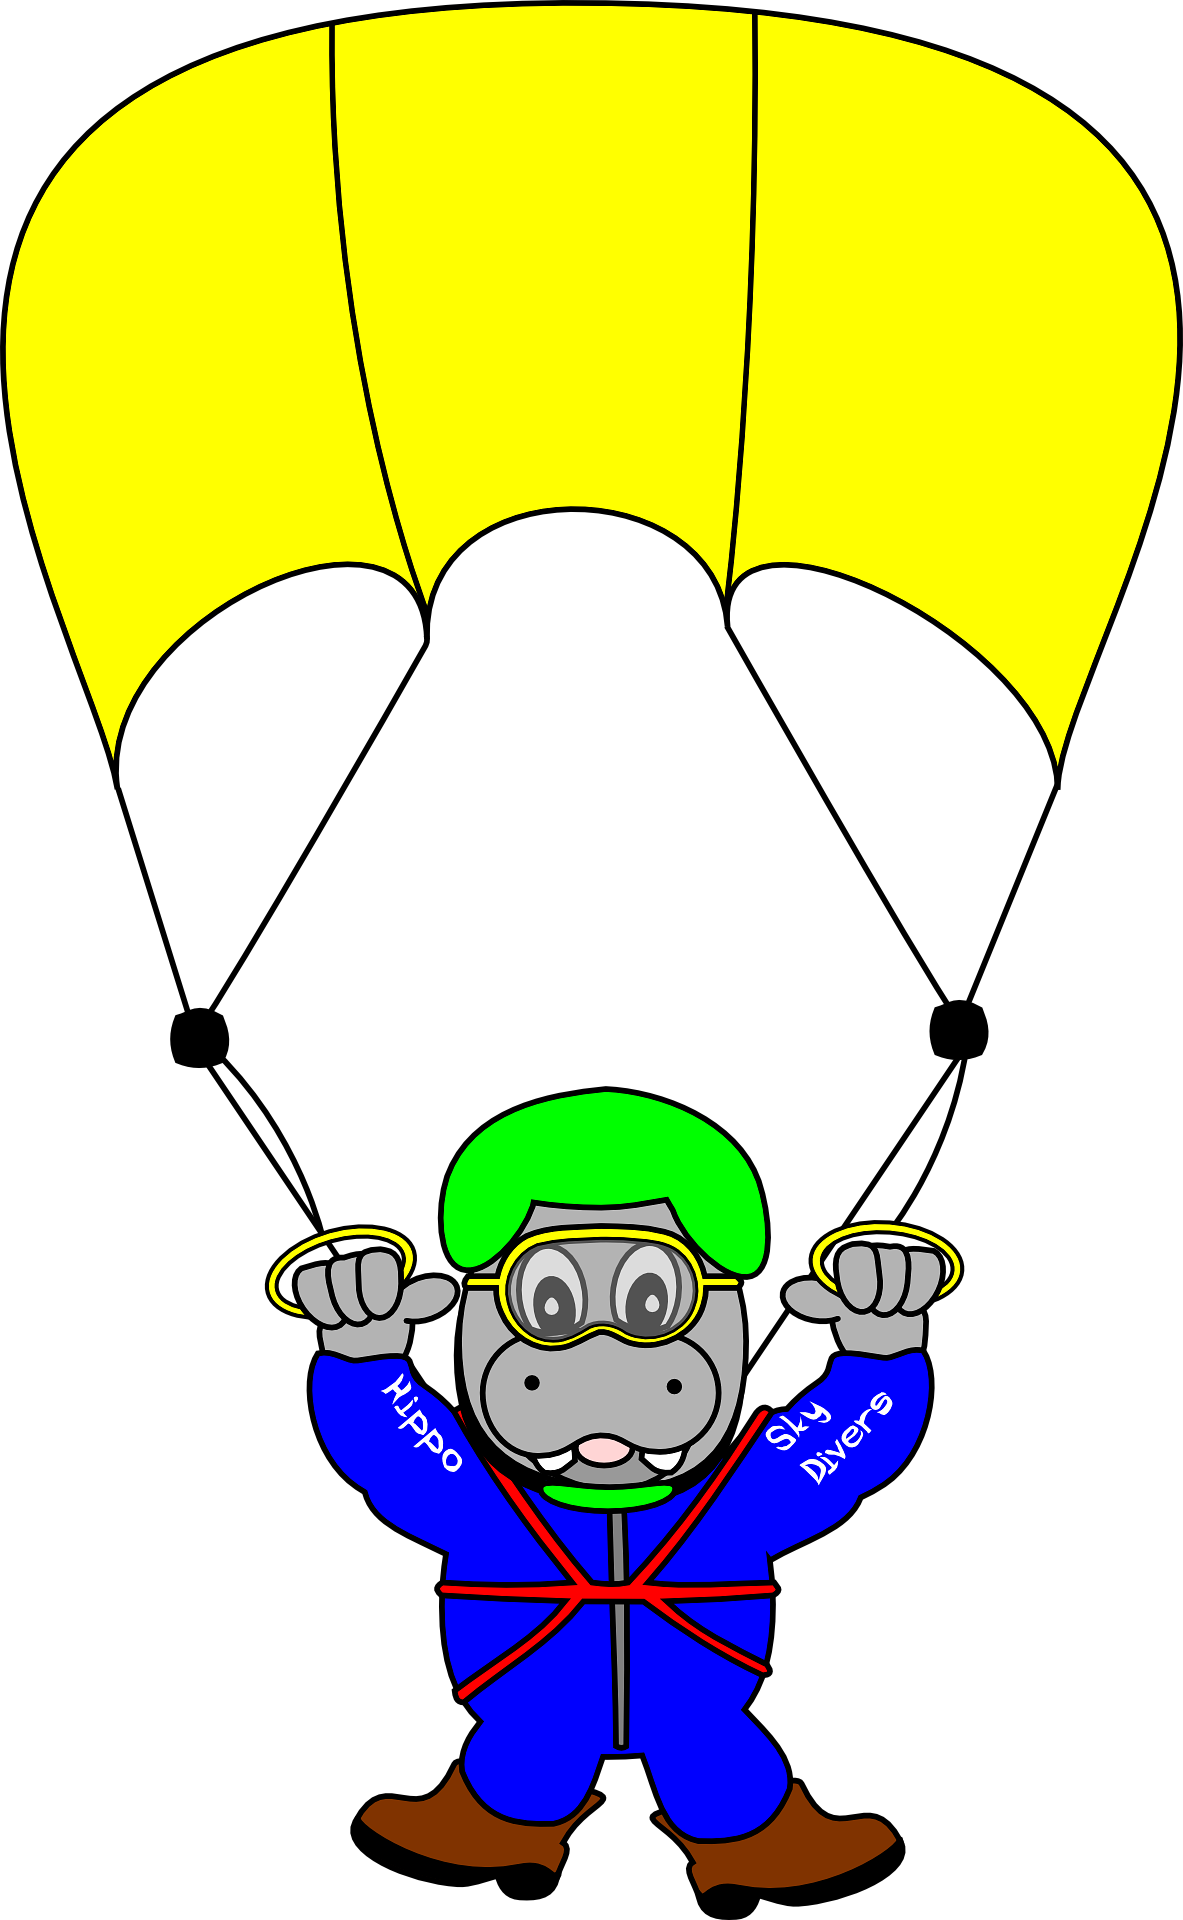
\includegraphics[height=0.39\columnwidth]{graphics/Chap09/skydiver-151230_1920.png}}%
\hfill%
    \caption[]{\textbf{Using a chute as a brake.} (a) A drag chute used for braking the \href{https://www.youtube.com/shorts/RwuI88iHeFo?t=33&feature=share}{Space Shuttle Endeavor}; image complements of \href{https://www.alamy.com/stock-photo/drag-chute-deployed.html?sortBy=relevant}{Almany} and (b) a parachutist; image complements of \href{https://pixabay.com/vectors/skydiver-fun-hippo-skydiving-151230/}{pixabay}.}
    \label{fig:DragParaChutes}
\end{figure}


\section{Let's Start Simple: One equation, One Unknown, One Derivative}

Our mission is to understand how ODEs can be used to model physical phenomena and how ``to solve'' some of the simplest possible ODEs. In fact, part of our mission is to understand what it even means to be a solution to an ODE.

\bigskip

\begin{factColor}{Four Models of Chutes}{ChuteModels}

We use Newton's Law, $F = m a$, written as $m \frac{dv(t)}{dt} = F$ to model an object braking under air resistance\footnote{The video \href{https://youtu.be/ym1hqL4UX3I}{Physics of a Parachute} by EA Reach provides an explanation of drag, aka air resistance. The only significant error in the video is the claim that the opening of a parachute ``initially causes a parachutist to move upward until gravity gradually takes over.''. While it surely feels that way to a parachutist, our senses often lie to us. Can you explain the feeling? The key is in Fig.~\ref{fig:Parachutist}-(b).} while rolling on flat ground and an object falling vertically under the combined influence of gravity and air resistance. In the following, $v$ (m/s) is the velocity of the object, $m$ (kg) is the mass, $\kappa$ (units depend on the model) is a drag coefficient, and $g$ (m/s$^2$) is the gravitational constant. 

 \begin{enumerate}
\renewcommand{\labelenumi}{(\alph{enumi})}
\setlength{\itemsep}{.2cm}
    \item \textbf{Model 1: Parallel Motion, Linear Drag:} $m \frac{dv(t)}{dt} =  - \kappa v(t), ~~v(t_0) = v_0$.

    \item \textbf{Model 2: Parallel Motion, Quadratic Drag:} $m \frac{dv(t)}{dt} =  - \kappa v^2(t), ~~v(t_0) = v_0$.

    \item \textbf{Model 3: Vertical Motion, Linear Drag:} $m \frac{dv(t)}{dt} = - \kappa v(t)- mg, ~~v(t_0) = v_0$.

    \item \textbf{Model 4: Vertical Motion, Quadratic Drag:} $m \frac{dv(t)}{dt} = \kappa v^2(t)-mg, ~~v(t_0) = v_0$.
\end{enumerate}
The term ``$v(t_0) = v_0$'' is called the \textbf{initial condition} of the differential equation. We understand intuitively that the velocity of a ball at some future time depends on its velocity when it leaves our hand. For example, if you drop a ball at rest versus tossing it in the air at one meter per second, you know that its evolution will be different. Yet, the moment the ball leaves your hand, the physics is the same: the ball evolves under the action of gravity and air resistance.\\

Regarding the signs in Models 2 and 4, the correct model for drag is $-\kappa |v(t)|\cdot v(t)$, so that the \textbf{drag force acts opposite to the direction of motion}. For the space shuttle, we can assume that it is moving left to right at touchdown, and hence $v(t)>0$. Therefore, the model for drag simplifies to $ - \kappa v^2(t)$. For a parachutist, however, $v(t)<0$, and therefore, the model for drag simplifies to $+\kappa v^2(t)$, where the plus sign is included to emphasize that the drag force is acting ``opposite to the downward force of gravity'' for the parachutist.

\bigskip
\textbf{Note:} The \textbf{order of an ordinary differential equation} is the degree of the highest derivative appearing in the equation. A \textbf{homogeneous ordinary differential equation (ODE)} is a type of differential equation in which every term is a function of the dependent variable and its derivatives. In particular, there are no terms that are just constants or functions of the independent variable alone. Hence, in the above, Model 1 is a first-order linear homogeneous ODE and Model 2 is a first-order nonlinear homogeneous ODE. Models 3 and 4 are first-order ODEs, but they are not homogeneous due to the inclusion of gravity in the model. Models that are not homogeneous are \textbf{inhomogeneous}, but if you say, \textbf{non-homogeneous}, everyone will understand you just fine.
    
\end{factColor}


\bigskip



\emstat{\textbf{Informal Definition of a Solution:} A differentiable function of time, $\varphi(t)$, is a solution to the ODE $\frac{dx(t)}{dt} =  f(x(t)), ~~x(t_0) = x_0$ if (i) it satisfies the initial condition, meaning, $\varphi(t_0) = x_0$, and (ii) it and its derivative together satisfy $\frac{d \varphi(t)}{dt} =  f( \varphi(t) )$, i.e., the left side equals the right side, as in any equation! \\

\textbf{Note:} For  $\frac{dx(t)}{dt} =  f(x(t))~~x(t_0) = x_0$, it is common practice to denote the solution by $x(t)$, the variable used in writing down the ODE, instead of using a different variable name, such as $\varphi$. For the drag chute and parachute models in Fact~\ref{thm:ChuteModels}, we'll consequently denote their solutions by $v(t)$. }

\bigskip

\subsection{Analytical Solutions via Antiderivatives}

\begin{example} 
\label{eq:ChuteODE01}
Compute and plot a solution to the first-order linear homogeneous ordinary differential equation, 
\begin{equation}
\label{eq:1stOrderLinearHomogeneous}
    m \frac{dv(t)}{dt} =  - \kappa v(t), ~~v(t_0) = v_0.
\end{equation}
    
\end{example}
\textbf{Solution:} \Ans~ $v(t)  = v_0 \cdot e^{ -\frac{\kappa}{m} \cdot \left( t - t_0 \right)}.$\\

First, we write $v$ in place of $v(t)$ and replace $dt$ with $d \tau$. Why? The next steps will be more clear when we use something other than $t$ as the dummy variable of integration. Proceeding, 
\begin{align*}
     \frac{dv}{d \tau} &=  - \frac{\kappa}{m} v\\
     & \Updownarrow  ~~~~~(\text{multiply both sides by } \frac{d \tau}{v})\\
    \frac{dv}{d \tau} \cdot \frac{d \tau}{v} &=  - \frac{\kappa}{m} v \cdot \frac{d \tau}{v} \\
     & \Updownarrow \\
    \frac{dv}{v}&=  - \frac{\kappa}{m} \, d \tau.\\     
\end{align*}
We now have $v$ on one side of the equation and $\tau$ on the other side. It is for this reason that the method is called \textbf{separation of variables}. We next integrate both sides to obtain
$$ \int_{v_0}^{v(t)}  \frac{dv}{v}=  - \frac{\kappa}{m} \int_{t_0}^t  \, d \tau ~~(\text{this is why we wanted $\tau$ instead of $t$ as the independent variable}).$$
In the above, $t_0$ is the time the shuttle Endeavor touches the runway, and $v_0=v(t_0)$ is the initial velocity of Endeavor at touchdown; often, we take $t_0=0$, but we could also use a different time reference, such as the time since the shuttle reentered the atmosphere.\\

We know antiderivatives for both integrands, giving us
\begin{align*}
\ln(v)~\bigg|_{v_0}^{v(t)}  &=  -\frac{\kappa}{m} \cdot \tau~\bigg|_{t_0}^t \\
                                & \Updownarrow  ~~(\text{using }  \ln(v(t)) - \ln(v_0) = \ln\left( \frac{v(t)}{v_0} \right) \\
 \ln\left( \frac{v(t)}{v_0} \right)   &= -\frac{\kappa}{m} \cdot \left( t - t_0 \right) \\     
  & \Updownarrow   ~~(\text{take exponential of both sides})\\
   \frac{v(t)}{v_0} &= e^{ -\frac{\kappa}{m} \cdot \left( t - t_0 \right)} \\
    & \Updownarrow  ~~(\text{multiply both sides by }v_0) \\ 
    v(t) & = v_0 \cdot e^{ -\frac{\kappa}{m} \cdot \left( t - t_0 \right)}.
\end{align*}

This gives us the general solution to the ODE as,
\begin{equation}
    \label{eq:ODEHorizontalLinearDrag}
    \setlength{\fboxrule}{2pt} % Adjust the thickness of the border
    \fcolorbox{brightblue}{lightblue}{%
    \addtolength{\fboxsep}{5pt} % Padding around the formula
    \( m \frac{dv(t)}{dt} =  - \kappa v(t),~~  v(t_0)=v_0  \) \(\Longleftrightarrow v(t) = v_0 \cdot e^{ -\frac{\kappa}{m} \cdot \left( t - t_0 \right)} \),
    }
\end{equation}
which was the main point of the exercise. \\

\textbf{Bonus:} Let's do a bit more with it because we are engineers. What should the value of $\kappa$ be so that in 3,000 m, the speed of the space shuttle is reduced to 10\% of its landing speed of $120$~m/s  (over 400 km/hr), given that it weighs $78,000$~kg? The assumption is that friction brakes could take over at that point. 

Well, distance is the integral of speed. If we take $t_0= 0$, we have
$$x(t) = \int_0^T  v_0 \cdot e^{ -\frac{\kappa}{m} \cdot \tau} \, d \tau = v_0 \frac{m}{\kappa} \cdot \left(1 - e^{ -\frac{\kappa}{m} \cdot T} \right),$$
where $T$ is the time it takes to reduce the velocity to $0.1 v_0$. Using our expression for velocity, we compute that $T$ satisfies, 
$$0.1 v_0 = v_0 \cdot e^{ -\frac{\kappa}{m} \cdot T} \iff e^{ -\frac{\kappa}{m} \cdot T}  = 0.1$$

Substituting this into our formula for distance, we have that 
$$ 3000 =  v_0 \frac{m}{\kappa} \cdot \left(1 - e^{ -\frac{\kappa}{m} \cdot T} \right) = v_0 \frac{m}{\kappa}\cdot \left(1 - 0.1 \right)\implies \fbox{$ \kappa = \frac{0.9\cdot v_0 \cdot m}{3000} = 2808$ }.$$




A plot of $v(t)$ vs $t$ is given in Fig.~\ref{fig:SpaceShuttleDragChutes}-(a). The red dot marks the time at which the shuttle has traveled 3~km and reduced its speed to 12 m/s or approx 27 mph. The runway is 4km long. 


\Qed



\bigskip


\begin{table}[h!]
\centering
\caption{Everyday Speed Examples in mph and m/s. For a quick conversion, using a factor of two is not bad, while $2.2$ and $0.45$ get you even closer.}
\begin{tabular}{@{}lcc@{}}
\toprule
\textbf{Example} & \textbf{Speed (mph)} & \textbf{Speed (m/s)} \\ \midrule
Average Human Walking & 3.1 & 1.4 \\
Cyclist (moderate speed) & 15 & 6.7 \\
Car (city driving) & 30 & 13.4 \\
Car (highway speed) & 60 & 26.8 \\
Propeller Airplane & 150 & 67.1 \\
Commercial Jet & 550 & 245.9 \\
High-Speed Train & 200 & 89.4 \\
Cheetah & 75 & 33.5 \\
Sound Speed at Sea Level & 767 & 343 \\
\bottomrule
\end{tabular}
\end{table}

\bigskip

\begin{figure}[htb]%
\centering
\subfloat[]{%
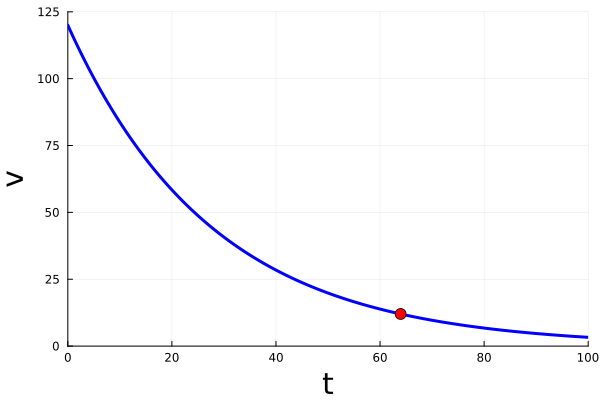
\includegraphics[width=0.45\columnwidth]{graphics/Chap09/SpaceShuttleLinearDragModel.png}}%
\hfill
\subfloat[]{%
%\includegraphics[trim=left2 bottom2 right2 top2, clip, width=0.5\columnwidth]
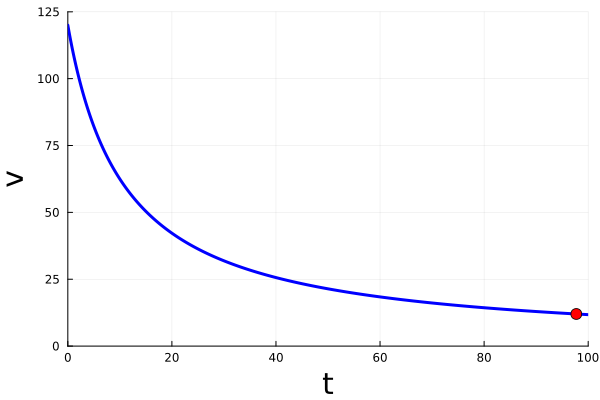
\includegraphics[width=0.45\columnwidth]{graphics/Chap09/SpaceShuttleNonlinearDragModel.png}}%
\hfill
    \caption[]{Velocity profiles of the Space Shuttle Endeavor braking with a chute in meters per second (m/s). (a) Linear drag model. (b) Nonlinear drag model. The linear model optimistically predicts that Endeavor's speed is reduced to 12 m/s approximately 30 seconds sooner than the (probably more accurate) nonlinear drag model.}
    \label{fig:SpaceShuttleDragChutes}
\end{figure}


\bigskip
\textbf{Videos on the Method of Separation of Variables}
\begin{itemize}
    \item \href{https://youtu.be/DL-ozRGDlkY}{Separable differential equations introduction: First order differential equations} by Khan Academy.

    \item \href{https://youtu.be/C7nuJcJriWM}{Separable First Order Differential Equations - Basic Introduction} by The Organic Chemistry Tutor.

    \item \href{https://youtu.be/7Y-frhf-1Zk}{Separation of Variables // Differential Equations} by Dr. Trefor Bazett.

\end{itemize}

\bigskip

\begin{example} 
\label{eq:ChuteODE02}
Compute and plot a solution to the first-order nonlinear, homogeneous ordinary differential equation,  
\begin{equation}
\label{eq:1stOrderNonlinearHomogeneous}
    m \frac{dv(t)}{dt} =  - \kappa v^2(t),~~v(t_0) = v_0.
\end{equation}
   
\end{example}
\textbf{Solution:} \Ans~ $v(t) = \frac{v_0}{1 + v_0 \cdot \frac{\kappa}{m} \cdot \left( t - t_0 \right)}$.\\

Things will be a bit more clear in the following steps if we write $v$ in place of $v(t)$ and replace $dt$ with $d \tau$. Doing so yields,
\begin{align*}
     \frac{dv}{d \tau} &=  - \frac{\kappa}{m} v^2\\
     & \Updownarrow ~~~  ~~(\text{multiply both sides by } \frac{d \tau}{v})\\
    \frac{dv}{d \tau} \cdot \frac{d \tau}{v} &=  - \frac{\kappa}{m} v^2 \cdot \frac{d \tau}{v}\\
     & \Updownarrow \\
    \frac{dv}{v^2}&=  - \frac{\kappa}{m} \, d \tau.\\     
\end{align*}
\textbf{Separation of variables:} We now have $v$ on one side of the equation and $\tau$ on the other side. We next integrate both sides to obtain
$$ \int_{v_0}^{v(t)}  \frac{dv}{v^2}=  - \frac{\kappa}{m} \int_{t_0}^t  \, d \tau.$$
In the above, $t_0$ is the time of touchdown, and $v_0=v(t_0)$ is the initial velocity of Endeavor at touchdown. We know antiderivatives for these two integrands, giving us
\begin{align*}
- \frac{1}{v}\bigg|_{v_0}^{v(t)} &=  -\frac{\kappa}{m} \cdot \tau~\bigg|_{t_0}^t \\
                                & \Updownarrow \\
-\left(\frac{1}{v(t)} - \frac{1}{v_0} \right)   &= -\frac{\kappa}{m} \cdot \left( t - t_0 \right) \\     
  & \Updownarrow   \\
   -\frac{1}{v(t)}  &=  -\frac{1}{v_0} -\frac{\kappa}{m} \cdot \left( t - t_0 \right)\\
    & \Updownarrow  ~~(\text{solve for }v(t))\\ 
    v(t) & = \frac{1}{\frac{1}{v_0} + \frac{\kappa}{m} \cdot \left( t - t_0 \right)} \\
     & \Updownarrow  \\
   v(t) & = \frac{v_0}{1 + v_0 \cdot \frac{\kappa}{m} \cdot \left( t - t_0 \right)}.   
\end{align*}

This gives us the general solution to the ODE as,
\begin{equation}
    \label{eq:ODEHorizontalLinearDragSolution}
    \setlength{\fboxrule}{2pt} % Adjust the thickness of the border
    \fcolorbox{brightblue}{lightblue}{%
    \addtolength{\fboxsep}{5pt} % Padding around the formula
    \( m \frac{dv(t)}{dt} =  - \kappa v^2(t),~~  v(t_0)=v_0  \) \(\Longleftrightarrow v(t) = \frac{v_0}{1 + v_0 \cdot \frac{\kappa}{m} \cdot \left( t - t_0 \right)}  \),
    }
\end{equation}
which was the main point of the exercise. \\

\textbf{Bonus:} Let's do a bit more with it because we are engineers. With this nonlinear model of drag, what should the value of $\kappa$ be so that in 3,000 m, the speed of the space shuttle is reduced to 10\% of its landing speed of $120$~m/s (over 400 km/hr), given that it weighs $78,000$~kg? The assumption, again, is that friction brakes could take over at that point. 

The time it takes to slow down to $0.1 v_0$ is
$$0.1 v_0 =  \frac{v_0}{1 + v_0 \cdot \frac{\kappa}{m} \cdot T} \implies 10 = 1+ v_0 \cdot \frac{\kappa}{m} \cdot T \implies T = \frac{9 m}{\kappa v_0}.$$

This time, integrating velocity to obtain distance  will require a u-substitution, $u = 1 + v_0 \cdot \frac{\kappa}{m} t$, $du =  v_0 \cdot \frac{\kappa}{m} \, dt$, giving, 
\begin{align*}
    x(T) &= \int_{t=0}^{t=T} \frac{v_0}{1 + v_0 \cdot \frac{\kappa}{m} \cdot t} \, dt \\[1em]
    &= \int_{u=1}^{u=10} \frac{m}{\kappa} \frac{1}{u} \, du \\[1em]
    &= \frac{m}{\kappa} \cdot \ln(10).
\end{align*}
Imposing $3000 =  \frac{m}{\kappa_{NL}} \cdot \ln(10) \implies \fbox{ $ \kappa = \frac{m}{3000} \cdot \ln(10) = 59.8 $ }$. A plot of $v(t)$ vs $t$ is given in Fig.~\ref{fig:SpaceShuttleDragChutes}-(b).\\

\textbf{Note:} The required drag coefficient predicted by the nonlinear model is very different from the value predicted by the linear model, $\kappa = 59.8$ versus $ \kappa = 2808$. This is because of the extra factor of $v$ in the nonlinear drag model, $\kappa\cdot v \cdot v$, versus the linear drag model $\kappa \cdot v$. Dividing the linear drag coefficient by 120 gives 23.4, which is in the same ballpark. When you understand that a linear approximation of $\kappa\cdot v \cdot v$ about the landing speed is $2 \kappa \cdot v_0 \cdot (v-v_0)$, the values match up even better, $\kappa = 59.8$ versus $ \kappa = 46.8$. 
\Qed

\bigskip

We now turn to analyzing the models for a parachutist\footnote{A ``parachutist'' is someone who is trained and experienced in the art of skydiving. They have likely completed many jumps and have received formal training and certification. On the other hand, a ``parachuter'' is someone who simply jumps out of a plane with a parachute, without necessarily having any formal training or experience.}, where gravity has an effect. The differential equations are now inhomogeneous. For the linear model, we need a new idea when seeking to compute a solution.


\begin{factColor}{Integrating Factors and Integration by Parts}{IntegratingFactors}
The concept of an \textbf{integrating factor} in solving differential equations and the technique of \textbf{integration by parts} in integral calculus are both based on the \textbf{product rule of differentiation}. 
\begin{enumerate}
    \item \textbf{Integration by Parts in Integral Calculus:}
    \begin{itemize}
        \item Integration by parts is a technique derived from the product rule of differentiation. It is used to solve integrals involving the product of two functions and is expressed as \( \int u \, dv = uv - \int v \, du \).
        \item It allows you to exchange the task of finding an antiderivative for $\int u \, dv$ for the ``hopefully'' easier task of finding an antiderivative for $\int v \, du$. 
        \item This formula is a direct consequence of the product rule. If you take the derivative of the product of two functions \( u\cdot v \) using the product rule and then integrate both sides, you arrive at the integration by parts formula.
    \end{itemize}
    
    \item \textbf{Integrating Factor in Differential Equations:}
    \begin{itemize}
        \item In the context of first-order linear differential equations, the integrating factor method involves finding a function (the integrating factor) that, when multiplied with the original differential equation, transforms the original ODE into a form where the left side becomes a total differential, as in $d\left(u\cdot v\right)$, making it trivial to integrate. The ``hope'' is that an antiderivative can be found for the right side of the equation.  
        \item For a differential equation of the form \( \frac{dy(t)}{dt} + P(t)y(t) = Q(t) \), an integrating factor is  \( e^{\int_{a}^t P(\tau) \, d\tau} \), for $a$ an arbitrary constant, because:
        \begin{itemize}
        \item Multiplying both sides of the ODE by  \( e^{\int_{a}^t P(\tau) \, d\tau} \) gives
        $$ \left(e^{\int_{a}^t P(\tau) \, d\tau}\right) \cdot \left(\frac{dy(t)}{dt} + P(t)y(t)\right) =\left( e^{\int_{a}^t P(\tau) \, d\tau} \right) \cdot Q(t).$$
            \item By the Chain Rule and the First Fundamental Theorem of Calculus, 
            $$\frac{d}{dt} \left(e^{\int_{a}^t P(\tau) \, d\tau}\right) = \left(e^{\int_{a}^t P(\tau) \, d\tau}\right) \cdot \frac{d}{dt}\int_{t_0}^t P(\tau) \, d\tau = e^{\int_{a}^t P(\tau) \, d\tau} \cdot P(t);$$
            \item By the Product Rule, 
            \begin{align*}
                \frac{d}{dt} \left( y(t) \cdot e^{\int_{a}^t P(\tau) \, d\tau} \right) &=\frac{dy(t)}{dt} \cdot \left(e^{\int_{a}^t P(\tau) \, d\tau} \right)+ y(t) \cdot \frac{d}{dt} \left( e^{\int_{a}^t P(\tau) \, d\tau} \right) \\[1em]
                &= \frac{dy(t)}{dt} \cdot e^{\int_{a}^t P(\tau) \,d\tau} + y(t) \cdot e^{\int_{a}^t P(\tau) \, d\tau} \cdot P(t);
            \end{align*}
            \item And hence, $e^{\int_{a}^t P(\tau) \, d\tau}  \cdot \left(  \frac{dy(t)}{dt} + P(t)y(t)\right) =  \frac{d}{dt} \left( y(t) \cdot e^{\int_{a}^t P(\tau) \, d\tau} \right) $ is a total differential, making it trivial to integrate (aka, anti-differentiate); and 
            \item Then, as in Integration by Parts, we ``hope'' that we can find an antiderivative for the right side of the equation, 
            $$Q(t) \cdot e^{\int_{a}^t P(\tau) \, d\tau}. $$
        \end{itemize}        
    \end{itemize} 
    \textbf{Note:} When computing the integrating factor, $e^{\int_{\bm{a}}^t P(\tau) \, d\tau}$, you are free to choose $\bm{a}$ to simplify the integral, $\int_{\bm{a}}^t P(\tau) \, d\tau$. Zero and minus infinity are often convenient values.
\end{enumerate}
   
\end{factColor}

\bigskip

\begin{example} 
\label{eq:ChuteODE03}
Compute and plot a solution to the first-order linear inhomogeneous ODE.
\begin{equation}
\label{eq:1stOrderLinearNonHomogeneous}
   m \frac{dv(t)}{dt} = - \kappa v(t) -  m g,  ~~v(t_0) = v_0.
\end{equation}
    
\end{example}
\textbf{Solution:} \Ans~ $v(t) =   v_0 e^{-\frac{\kappa}{m}(t - t_0)} - \frac{mg}{\kappa} \cdot \left( 1 - e^{-\frac{\kappa}{m}(t - t_0)} \right)$.

Given the differential equation \( m \frac{dv(t)}{dt} =- \kappa v(t) -   mg  \), we can rewrite it as,
$$ \frac{dv(t)}{dt} + \frac{\kappa}{m} v(t) = -g. $$
The solution to this equation can be found using an \textbf{integrating factor}, as explained in Fact~\ref{thm:IntegratingFactors}. In this case, $P(t) = \frac{\kappa}{m}$, which has antiderivative $ \frac{\kappa}{m}\cdot t + a$. Taking $a=0$ gives the integrating factor as 
$$ e^{\frac{\kappa}{m}t}. $$

As developed in Fact~\ref{thm:IntegratingFactors}, the integrating factor has the ``magical property'' that when we multiply both sides of the ODE by  \( e^{\frac{\kappa}{m}t} \), giving us,
$$ e^{\frac{\kappa}{m}t} \frac{dv(t)}{dt} + \frac{\kappa}{m} e^{\frac{\kappa}{m}t} v(t) = -g e^{\frac{\kappa}{m}t}, $$
the left side of the equation is equal to \( \frac{d}{dt} \left(e^{\frac{\kappa}{m}t} v(t) \right)\). Therefore, integrating both sides with respect to \( t \) gives,
$$ \int \frac{d}{dt} \left( e^{\frac{\kappa}{m}t} v(t) \right) dt = -\int g e^{\frac{\kappa}{m}t} dt. $$

Determining an antiderivative for the left side is now trivial, which was the job of the integrating factor. Determining an antiderivative for the right side is straightforward because it involves an exponential. 
Integrating and rearranging, we therefore obtain,
$$ e^{\frac{\kappa}{m}t} v(t) = -\frac{mg}{\kappa} \left( e^{\frac{\kappa}{m}t} - 1 \right) + C, $$
where \( C \) is the constant of integration. To find \( C \), we use the initial condition \( v(t_0) = v_0 \), per
$$ e^{\frac{\kappa}{m}t_0} v_0 = -\frac{mg}{\kappa} \left( e^{\frac{\kappa}{m}t_0} - 1 \right) + C. $$
Solving for \( C \) and then substituting back into the equation for \( v(t) \), yields the final solution,
$$ v(t) =v_0 e^{-\frac{\kappa}{m}(t - t_0)} - \frac{mg}{\kappa} \left( 1 - e^{-\frac{\kappa}{m}(t - t_0)} \right).$$

This gives us the general solution to the ODE as,
\begin{equation}
    \label{eq:ODEHorizontalLinearDragGeneralSolution}
    \setlength{\fboxrule}{2pt} % Adjust the thickness of the border
    \fcolorbox{brightblue}{lightblue}{%
    \addtolength{\fboxsep}{5pt} % Padding around the formula
    \( m \frac{dv(t)}{dt} =  mg - \kappa v(t),~~  v(t_0)=v_0  \) \(\Longleftrightarrow v(t) =  v_0 e^{-\frac{\kappa}{m}(t - t_0)} - \frac{mg}{\kappa} \left( 1 - e^{-\frac{\kappa}{m}(t - t_0)} \right)\).
    }
\end{equation}
The limit as $t \to \infty$ is called the ``terminal velocity''. No, it's not the speed that terminates a beginner parachuter. It's the steady-state speed reached by the parachutist,
$$ \lim_{t \to \infty} v(t) =  \lim_{t \to \infty} v_0 e^{-\frac{\kappa}{m}(t - t_0)} - \frac{mg}{\kappa} \left( 1 - e^{-\frac{\kappa}{m}(t - t_0)} \right) = -\frac{m g}{\kappa}.$$
From this, we see that if a 75 kg parachutist wants to land with a speed of $-2$m/s, they need a parachute that provides a drag coefficient of \fbox{$\kappa=367.88$}. A plot is given in Fig.~\ref{fig:Parachutist}-(a).

\Qed

\bigskip

\begin{figure}[htb]%
\centering
\subfloat[]{%
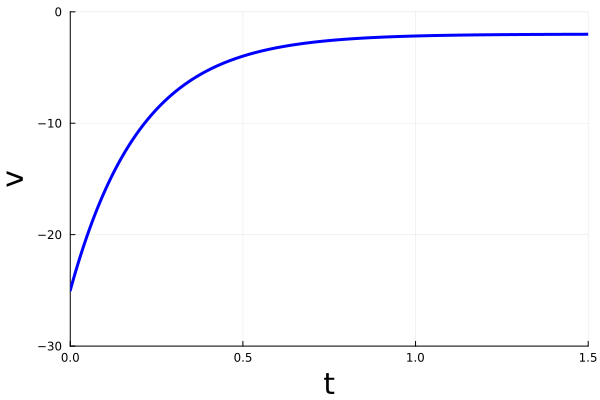
\includegraphics[width=0.45\columnwidth]{graphics/Chap09/ParachutistLinearDragModel.png}}%
\hfill
\subfloat[]{%
%\includegraphics[trim=left2 bottom2 right2 top2, clip, width=0.5\columnwidth]
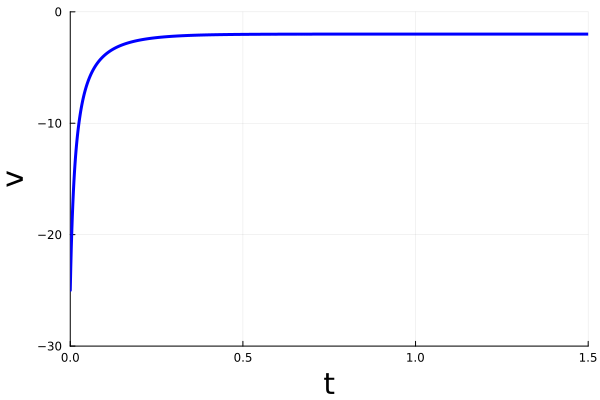
\includegraphics[width=0.45\columnwidth]{graphics/Chap09/ParachutistNonlinearDragModel.png}}%
\hfill
    \caption[]{Velocity profiles of parachutists, with an emphasis on when each model ``achieves a terminal velocity''. (a) Linear drag model. (b) Nonlinear drag model. The linear model predicts a more gentle deceleration to the terminal velocity. In practice, a chute does not open instantaneously, so the braking effect of a real parachute (with nonlinear drag) may not be as harsh as we are predicting!}
    \label{fig:Parachutist}
\end{figure}

\bigskip


\begin{example} 
\label{ex:ChuteODE04}
Compute and plot a solution to the first-order nonlinear, inhomogeneous ordinary differential equation,  
\begin{equation}
\label{eq:1stOrderNonlinearHomogeneousExercise}
    m \frac{dv(t)}{dt} =   \kappa v^2(t) - mg,~~v(t_0) = v_0.
\end{equation}    
\end{example}
\textbf{Solution:} \Ans~ A closed-form solution cannot be given in terms of elementary functions, as defined in \textgoth{Secrets of the Arcane} ~\ref{thm:ElementaryFunctions}. To prove this fact requires \href{https://en.wikipedia.org/wiki/Differential_Galois_theory}{Differential Galois Theory}, which few non-mathematicians acquire in their mathematical studies. Even though a closed-form solution cannot be found, we can still compute numerical solutions, as shown in Fig.~\ref{fig:Parachutist}-(b). Moreover, qualitative analysis of the equation can be done as in the video \href{https://youtu.be/3AIA1HBsTVI}{Parachute Physics} by 
LabRat Scientific. \\

So yes, we can still compute a terminal velocity, $v_{\rm ss}$. At the terminal velocity, $\frac{dv(t)}{dt} \equiv 0$. Using this as a definition, we have
$$\frac{dv(t)}{dt} \equiv 0 \implies  \kappa v^2_{\rm ss} = mg \implies  v_{\rm ss} = \sqrt{\frac{mg}{\kappa}}.$$
We can also turn it around to ``size the parachute'' because larger parachutes provide more air resistance. For a parachutist to land with a velocity of $v_{\rm ss}$ m/s implies 
$$ \kappa = \frac{mg}{v^2_{\rm ss}}.$$ 
For a parachutist with a mass of 75 kg and desiring a terminal velocity of -2 m/s, \fbox{$\kappa =  183.94$}. A plot is given in Fig.~\ref{fig:Parachutist}-(b).\\


\emstat{It's remarkable that, just by adding a constant term to the right side of an ODE with one derivative, one unknown, and one equation, we went from something solvable by an elementary method, namely separation of variables, to an ODE where it is provably impossible to write down an analytical solution. Now, go back and look at the ODEs we derived via Lagrange's method and ask yourself, what's the chance we can find an analytical solution to those equations? Ah, what is one in a googol (one in $10^{100})$?}


\Qed


\subsection{Numerical Solutions}



\subsubsection{Solving ODEs in Julia Using DifferentialEquations.jl}

Among the many powerful tools in Julia for solving Ordinary Differential Equations (ODEs) is the \texttt{DifferentialEquations.jl} package. This package provides a comprehensive suite of solvers and utilities for dealing with various types of differential equations. To begin, you need to define the differential equation in a function. For example, consider an ODE of the form \(\frac{dy}{dt} = f(y, t)\), where \(f\) is some function of \(y\) and \(t\). In Julia, you would define this as \texttt{function f(y, t)}. Next, you set the initial condition and the time span for which you want to solve the ODE. This is done by creating an \texttt{ODEProblem} object with your function, initial condition, and time span. Finally, you solve the ODE using the \texttt{solve} function from the package. This function takes the problem object and optionally a solver algorithm and other parameters. The result is a solution object that can be analyzed or plotted to understand the behavior of the system described by the ODE. For more information and examples, visit the \href{https://diffeq.sciml.ai/stable/}{DifferentialEquations.jl documentation}.




\subsubsection{Endeavor with a Linear Drag Model}

\begin{lstlisting}[language=Julia,style=mystyle]
# Import useful packages
using DifferentialEquations
using Plots 
gr()

# Space Shuttle Endeavor with Linear Drag Model
struct Params
    m::Float64      # Mass in kilograms
    kappa::Float64  # Drag coefficient
    g::Float64      # Acceleration due to gravity in m/s^2
end

# Initialize the Params structure with specific values
m = 78e3 # kg  78,000 kg or 39 metric tons
g = 9.81 # m/s^2
v0 = 120 # m/s
kappa = (0.9*v0*m)/3000; @show kappa
#
params = Params(m, kappa, g)

# define the ODE dv/dt = f(v,params,t)
function f(v, params, t)
    dv = -(params.kappa / params.m) * v
    return dv
end

# Set the initial condition as a vector!
v0 = 120 # m/s 
v0= [v0]

# Set the time interval
T = (0.0, 100) # 100 second simulation period?

# Setup the ODE problem with out-of-place function
problem = ODEProblem{false}(f, v0, T, params)

# solve the ODE problem using the Runge Kutta Tsitouras 5/4 Integrator
sol = solve(problem, Tsit5())

# plot the solution
p1 = plot(sol, lw=3, guidefont = 20,  xlabel="t", ylabel="v", legend=false, color=:blue)
ylims!(p1, (0, 125))

# e^{ -\frac{\kappa}{m} \cdot Tf}  = 0.1 <==> Tf = -(m/kappa)*log(0.1)
Tf = -(m/kappa)*log(0.1); @show Tf
p1 = scatter!(p1, [Tf], [0.1*v0], color=:red, markersize=6)
\end{lstlisting}
\textbf{Output} 
\begin{verbatim}
kappa = 2808
Tf = 63.960697027612376
\end{verbatim}



\subsubsection{Endeavor with a Nonlinear Drag Model}


\begin{lstlisting}[language=Julia,style=mystyle]
# Import useful packages
using DifferentialEquations
using Plots 
gr()

# Space Shuttle Endeavor with Nonlinear Drag Model
struct Params
    m::Float64      # Mass in kilograms
    kappa::Float64  # Drag coefficient
    g::Float64      # Acceleration due to gravity in m/s^2
end

# Initialize the Params structure with specific values
m = 78e3 # 78,000 kg 
g = 9.81
kappa = (m/3000)*log(10); @show kappa
params = Params(m, kappa, g)

# define the ODE dv/dt = f(v,params,t)
function f(v, params, t)
    dv = -(params.kappa / params.m) * v.^2
    return dv
end

# Set the initial condition as a vector!
v0 = 120 # m/s 
v0= [v0]

# Set the time interval
T = (0.0, 100) 

# Setup the ODE problem with out-of-place function
problem = ODEProblem{false}(f, v0, T, params)

# solve the ODE problem using the Runge Kutta Tsitouras 5/4 Integrator
sol = solve(problem, Tsit5())

# plot the solution
p1 = plot(sol, lw=3, guidefont = 20,  xlabel="t", ylabel="v", legend=false, color=:blue)

# e^{ -\frac{\kappa}{m} \cdot Tf}  = 0.1 <==> Tf = -(m/kappa)*log(0.1)
Tf = 9*m/(kappa*v0[1]); @show Tf
p1 = scatter!(p1, [Tf], [0.1*v0], color=:red, markersize=6)
ylims!(p1, (0, 125))
\end{lstlisting}
\textbf{Output} 
\begin{verbatim}
kappa = 59.867212417845195
Tf = 97.71625842823164
\end{verbatim}



\subsubsection{Parachutist with a Linear Drag Model}
\begin{lstlisting}[language=Julia,style=mystyle]
# Import useful packages
using DifferentialEquations
using Plots 
gr()

# Parachutist with a linear drag model
struct Params
    m::Float64      # Mass in kilograms
    kappa::Float64  # Drag coefficient
    g::Float64      # Acceleration due to gravity in m/s^2
end

#vTerminal =  -\frac{m g}{\kappa}

# Initialize the Params structure with specific values
m = 75 # kg
g = 9.81 # m/s^2

vTerminal = -2 # m/s
kappa = -m*g/vTerminal; @show kappa
params = Params(m, kappa, g)

# define the ODE dv/dt = f(v,params,t)
function f(v, params, t)
    dv = -params.g .-(params.kappa / params.m) * v
    return dv
end

# Set the initial condition as a vector
v0 = -25 # m/s speed when chute is opened
v0= [v0]

# Set the time interval
T = (0.0, 1.5) # 

# Setup the ODE problem with out-of-place function
problem = ODEProblem{false}(f, v0, T, params)

# solve the ODE problem using the Runge Kutta Tsitouras 5/4 Integrator
sol = solve(problem, Tsit5());

# plot the solution
p1 = plot(sol, lw=3, guidefont = 20,  xlabel="t", ylabel="v", legend=false, color=:blue)
ylims!(p1, (-30, 0))
\end{lstlisting}
\textbf{Output} 
\begin{verbatim}
kappa = 367.875
\end{verbatim}



\subsubsection{Parachutist with a Nonlinear Drag Model}

\begin{lstlisting}[language=Julia,style=mystyle]
# Import useful packages
using DifferentialEquations
using Plots 
gr()

# Parachutist with a nonlinear drag model
struct Params
    m::Float64      # Mass in kilograms
    kappa::Float64  # Drag coefficient
    g::Float64      # Acceleration due to gravity in m/s^2
end

#vTerminal =  -\frac{m g}{\kappa}

# Initialize the Params structure with specific values
m = 75 # kg
g = 9.81 # m/s^2


vTerminal = -2 # m/s
kappa = m*g/(vTerminal^2); @show kappa
params = Params(m, kappa, g)

# define the ODE dv/dt = f(v,params,t)
function f(v, params, t)
    dv =  dv = -params.g .-((params.kappa / params.m) .* abs.(v).*v)
    return dv
end

# Set the initial condition as a vector
v0 = -25 # m/s speed when chute is opened
v0= [v0]

# Set the time interval
T = (0.0, 1.5) # 

# Setup the ODE problem with out-of-place function
problem = ODEProblem{false}(f, v0, T, params)

# solve the ODE problem using the Runge Kutta Tsitouras 5/4 Integrator
sol = solve(problem, Tsit5());

# plot the solution
p1 = plot(sol, lw=3, guidefont = 20,  xlabel="t", ylabel="v", legend=false, color=:blue)
ylims!(p1, (-30, 0))
\end{lstlisting}
\textbf{Output} 
\begin{verbatim}
kappa = 183.9375
\end{verbatim}

\subsection{Finite Escape Time}

The ODEs we have investigated so far have solutions that exist for all $t\ge 0$. This is NOT always the case. Consider 
\begin{equation}
    \frac{dx(t)}{dt} = 1 + x^2(t),
\end{equation}
with initial condition $x_0 = x(0)=0$. Then, using the method of separation of variables, we arrive at
\begin{align*} 
\frac{1}{1+x^2}\, dx &= d \tau \\
  & \Updownarrow   \\
\int_0^{x(t)}\frac{1}{1+x^2}\, dx &= \int_0^t \, d\tau \\
  & \Updownarrow   \\
\atan(x(t)) &= t \\
    & \Updownarrow   \\
    x(t) &= \tan(t).
\end{align*}
We know the function $\tan(t)$ has a vertical asymptote at $\frac{\pi}{2}$, that is, 
$$\lim_{t \to\frac{\pi}{2}^-} \tan(t) = \infty.$$
When the solution of the ODE has a vertical asymptote, we say that the ODE itself has a \textbf{finite escape time}: in finite time, the solution of the ODE ceases to exist; said another way, the solution explodes to $\pm \infty$ at a finite time called $t_{\rm escape}$. As you might imagine, finite escape times drive a numerical solver crazy.

\bigskip

\begin{lstlisting}[language=Julia,style=mystyle]
# Import useful packages
using DifferentialEquations
using Plots 
gr()

# Finite Escape Time

# define the ODE dv/dt = f(v,params,t)
function f(x,~, t) # If there are no paramters to pass, use a tilde
    dx = 1 .+ x.^2 # Function is vectorized
    return dx
end

# Set the initial condition as a vector
x0 = 0.0 # m/s
x0= [x0]

# Set the time interval
T = (0.0, 3) 

# Setup the ODE problem with out-of-place function
problem = ODEProblem{false}(f, x0, T)

# solve the ODE problem using the Runge Kutta Tsitouras 5/4 Integrator
sol = solve(problem, Tsit5());

# plot the solution
plot(sol)
\end{lstlisting}
\textbf{Output} 
\begin{verbatim}
Warning: dt(4.440892098500626e-16) <= dtmin(4.440892098500626e-16) at t=1.57071147677680
96. Aborting. There is either an error in your model specification or the true solution 
is unstable.
\end{verbatim}
\emstat{By ``unstable'', the solver means ``numerically unstable''. For you, it means the solutions blew up, and you need to decide if that is a ``feature'' or a ``bug''! In our case, it is not a bug in the code. It is a feature of the model we are trying to simulate. While it may not be a desirable feature, the finite escape time is inherent in the ODE itself and has nothing to do with the capabilities of the numerical solver. If we had set the time interval to any value $0< T < \frac{\pi}{2}$, the solver would have found a very good approximation of the solution. In the output's first line, the solver tells us it encountered a problem at $ t=1.5707114767768096$, which is very close to $\frac{\pi}{2}$.}

\subsection{One-Dimensional ODE with Multiple Solutions}
\label{sec:ODEwithInfiniteSolutions}

So far, we have associated a single solution to each ODE we have solved. Some nonlinear ODEs have more than one solution. These solutions can vary based on initial conditions or the nature of the equation itself. Here, we present a simple example of a one-dimensional ordinary differential equation (ODE) that exhibits multiple solutions.

Consider the differential equation
\begin{equation}
\label{eq:ODEwithNonuniqueSolutions}
    \frac{dx(t)}{dt} = \left(x(t)\right)^{2/3}, ~x(0)=0.
\end{equation}
\textbf{The right side of this ODE, $\bm{x^{2/3} = \sqrt[3]{x^2}}$, is notable because it is not differentiable at $\bm{x=0$}.} Indeed,
$$ \frac{d}{dx} \left( x^{2/3} \right)= \frac{2}{3}x^{ -\frac{1}{3}} = \frac{2}{3} \frac{1}{ \sqrt[3]{x}}$$
blows up at the origin. 

In terms of solutions, the trivial solution,
\begin{equation}
    x(t) \equiv 0
\end{equation}
satisfies the ODE and the initial condition. 
Surprisingly, there are other (non-trivial) solutions as well. For instance, the function $\varphi:[0, \infty) \to \real$ by
\begin{equation}
   \varphi(t) = \frac{t^3}{27},
\end{equation}
also satisfies the initial condition and the differental equation. Indeed,
\begin{itemize}
    \item $\frac{d}{dt} \varphi(t) =\frac{d}{dt} \frac{t^3}{27} = \frac{t^2}{9} $, and
    \item $\left(\varphi(t)\right)^{2/3} = \left(\left(\frac{t}{3}\right)^3\right)^{2/3} = \left(\frac{t}{3}\right)^2 = \frac{t^2}{9}.$
\end{itemize}

Perhaps even more mind-blowing\footnote{Why is this mind-blowing? Suppose you are building a gadget and through much labor, you show that one of its variables satisfies \eqref{eq:ODEwithNonuniqueSolutions}. Then the variable behaves almost like something ``random'' because, at any moment in time, the ``universe'' rolls a die, chooses $c>0$, and spookily produces a non-zero solution. Wild!}, for all constants $c>0$,
\begin{equation}
\label{eq:SpookyODEsolution}
   \varphi_c(t) = 
    \begin{cases} 
      0 & \text{if } t < c, \\
      \frac{(t-c)^3}{27} & \text{if } t \ge c,
    \end{cases}
\end{equation}
is also a solution. This example illustrates that some differential equations, particularly those where the right side is not everywhere continuously differentiable, can have multiple solutions. Understanding the criteria under which a unique solution exists is crucial in the study of ODEs. We address this in Chapter~\ref{sec:ExistenceUniquenessSolutionsODEs}.

\subsection{(Optional Read:) Can an ODE Have No Solution?}
\label{sec:ODEwithNoSolutions}

You see this question a lot on the internet, so we thought to address it by giving various examples. If they are all a bit wacky, that's a sign that most ODEs do have a solution.
 \begin{enumerate}
\renewcommand{\labelenumi}{(\alph{enumi})}
\setlength{\itemsep}{.2cm}
    \item $\left(\frac{dx(t)}{dt}\right)^2 + 1 = 0$ does not have a real solution for any initial condition for the same reason that $y^2+1 = 0$ has no real solutions.

    \item  $\frac{dx(t)}{dt} = \frac{1}{x(t)}$ does not have a solution for the initial condition $x(0) = 0$ because the right side of the ODE blows up at $x(t)=0$.

        \item  $\frac{dx(t)}{dt} = \begin{cases}
    1 & x \in \rat \\
    0 & \text{otherwise},         
    \end{cases}$ does not have a solution for any initial condition because the function on the right side of the ODE is not Riemann integrable. Why is that a problem? By the First Fundamental Theorem of Calculus, if the equation has a solution $x(t)$, then it must be an antiderivative of $x'(t)$, meaning that $x(t) = x(a) + \int_a^t x'(\tau)\, d\tau$. But for that to hold, we need to make sense of the integral. Because we only know Riemann Integration, we are stuck. Now, if you learn the Lebesgue Integral, you have a way out of this corner.
\end{enumerate}

The following result comes from Functional Analysis and Topology, branches of mathematics that math majors take their senior year or in grad school. It is only included here to underline that any ODE that may be of interest to an engineer can be proven to have a solution, justifying the wackiness of our ``counter examples.''\\

\emstat{\textbf{[Peano's Existence Theorem]}
Let \( G \) be an open set in \( \mathbb{R} \times \mathbb{R}^n \) and let \( f: G \to \mathbb{R}^n \) be a continuous function. If \( (t_0, x_0) \) is a point in \( G \), then there exists an interval \( I \) containing \( t_0 \) and a function \( x: I \to \mathbb{R}^n \) that is a solution to the initial value problem
\begin{equation}
    \frac{dx}{dt} = f(t, x), \quad x(t_0) = x_0.
\end{equation}
}

\begin{proof}
The proof of Peano's Existence Theorem is based on the application of the Arzelà–Ascoli theorem and Schauder's fixed point theorem. The idea is to construct a sequence of approximate solutions using successive approximations and show that this sequence has a convergent subsequence that converges to an actual solution of the differential equation. The continuity of \( f \) ensures that the sequence of approximate solutions is equicontinuous and uniformly bounded, which allows the application of the Arzelà–Ascoli theorem.
\end{proof}


\subsection{(Optional Read:) The Independent Variable in an ODE can be any Strictly Increasing Quantity}

The study of heat conduction is a fundamental aspect of thermodynamics and continuum mechanics. In particular, one-dimensional steady-state heat conduction can be modeled using a \textbf{second-order} ordinary differential equation. This model provides insights into how temperature varies along a rod or a similar object when the system has reached a steady state. If time were also considered, we would have a PDE.

Consider a long, thin rod of length \( L \), with thermal conductivity \( k \), and wrapped in thermal insulation along its length, except at the ends. The rod is heated at one end and cooled at the other, creating a temperature gradient along its length. Let $x$ be a position along the rod and $T(x)$ the temperature at the point $x$. The temperature distribution \( T(x) \) along the rod is described by the steady-state heat equation,
\begin{equation}
    -k \frac{d^2T}{dx^2} = 0,
\end{equation}
where \( k \) is the thermal conductivity of the material. The boundary conditions might be, for example, \( T(0) = T_0 \) (temperature at the heated end) and \( T(L) = T_L \) (temperature at the cooled end). 

The general solution to this differential equation is an affine (aka, linear plus a constant) temperature profile,
\begin{equation}
    T(x) = C_1 x + C_2,
\end{equation}
where \( C_1 \) and \( C_2 \) are constants determined by the boundary conditions. For the given boundary conditions, the solution becomes,
\begin{equation}
    T(x) = \frac{T_L - T_0}{L}x + T_0.
\end{equation}
This equation describes a linear temperature gradient from the heated end to the cooled end of the rod. While the examples we study will mostly have time as the independent variable, you will encounter various independent variables in other engineering courses. 

\begin{figure}[htb]%
\centering
\subfloat[]{%
%\includegraphics[trim=7cm 1cm 7cm 1cm, clip, width=0.45\columnwidth]
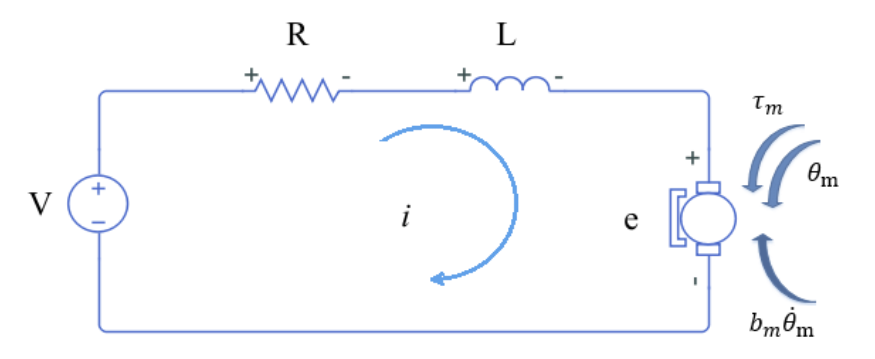
\includegraphics[width=0.55\columnwidth]{graphics/Chap09/CircuitModelDCmotor.png}}%
%\hfill%
\hspace{.3cm}
\subfloat[]{%
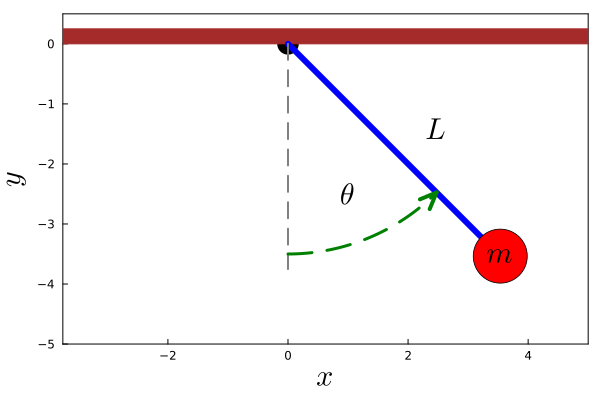
\includegraphics[ width=0.35\columnwidth]{graphics/Chap06/Pendulum.png}}%
\hfill
\caption[]{(a) A \href{https://www.researchgate.net/figure/Circuit-model-of-DC-motor_fig4_338420606}{circuit model of DC motor} by Research Gate. (b) The classic pendulum formed by a massless rod with a point mass attached at its end from Fig.~\ref{fig:SimplestDynamics}. The torque from the motor can used to achieve a desired behavior, such as balancing the pendulum in the upright position. \textbf{Notice the clash in notation, where ME-types use $L$ for length and EE-types use $L$ for inductance. This is very common and you have to learn how to navigate it.} In the text, we add a subscript $_p$ to the parameters of the pendulum and a subscript $_m$ to the parameters of the motor.}
    \label{fig:DCmotorAndPendulum}
\end{figure}

\section{Higher-order ODEs and a Direct Current (DC) Motor Model}

Most models of physical systems involve more than one derivative, or more than one variable, or both! Fig.~\ref{fig:DCmotorAndPendulum}-(b) shows the pendulum we studied in Chapter~\ref{sec:LagrangianDynamics}. Its differential equation is 
\begin{equation}
\label{eq:DddotqPendulumTake02}
   m_p \cdot L_p^2 \cdot \ddot{\theta} + m_p \cdot g\cdot L_p \cdot \sin(\theta)= \tau_p,
\end{equation}
where $\tau_p$ is the torque applied to the pendulum at the revolute joint. This is an example of a \textbf{second-order ODE in a single variable}, $\theta$. It is second order because the second derivative, $\ddot{\theta}$, appears in the model.

\begin{center}
\setlength{\fboxrule}{2pt}  % Setting the thickness of the border line
   \fbox{ \parbox{0.9\linewidth}{
   \vspace{.15cm} 
\textcolor{blue}{\bf This section aims to show that real differential equations typically have higher order than one and contain multiple variables. In other words, higher-order ODEs are not just a mathematical curiosity invented to torture young learners. If you are already convinced of this, then go straight to Definition~\ref{def:nthOrderODE} and then move on. If you need more convincing, or you just want to see how motors can be modeled and integrated with robot arms, then read on.}}
\vspace{.15cm} 
}
\end{center}

Fig.~\ref{fig:DCmotorAndPendulum}-(a) shows a standard circuit representation of a DC motor; more comprehensive treatments can be found in \href{https://ctms.engin.umich.edu/CTMS/index.php?example=MotorSpeed&section=SystemModeling}{DC Motor Speed: System Modeling} by the MathWorks (creator of MATLAB) and \href{https://youtu.be/GQatiB-JHdI}{How does an Electric Motor work? DC Motor explained} by The Engineering Mindset. Using \href{https://en.wikipedia.org/wiki/Kirchhoff%27s_circuit_laws}{Kirchoff's Current and Voltage Laws}\footnote{You can learn these in Michigan's EECS 215 Introduction to Electronic Circuits, EECS 314 Electrical Circuits, Systems, and Applications, or ROB 310 Robot Sensors and Signals.}, its model can be written as 
\begin{equation}
\label{eq:DddotqPendulumTake03}
   L_m \frac{d i}{dt} + R_m i = V - b_m \dot{\theta}_m,
\end{equation}
where $\theta_m$ is the angle of the motor's shaft, $L_m$ is the inductance of the motor's windings and $R_m$ is their resistance, $V$ is the DC source voltage applied to the motor, and $ b_m \dot{\theta}$ represents the ``back emf'' (Back Electromotive Force\footnote{The back (or counter) electromotive force (emf) is the voltage generated by a running motor that acts to counter the supplied voltage. In the simple case of a permanent-magnet DC motor, it is proportional to the rotational speed of the motor.}). The output shaft of the motor is typically connected to the revolute joint of the pendulum through some sort of gearing that imposes 
$$ \theta_m = N \theta,$$
where $N$ is the gear ratio, which could be in the range of 100. Gearing is needed because typical motors are efficient when spinning fast and producing low torque, while most robotics applications require high torque and low speed! \textbf{The current of the motor is now a second variable in the differential equations modeling the overall system.} The torque produced by a DC motor is proportional to the current, $\tau_m = K_m \cdot i$, where $K_m$ is called the motor torque constant. 

We have presented these details for two reasons:
\begin{itemize}
    
    \item The differential equations you will encounter in engineering come from physical systems. Each discipline has its collection of important differential equation models. You typically do not learn how to develop the models in a mathematics course. Your author learned how to model through courses in Physics, Chemistry, EE, and ME (Robotics did not exist as an academic discipline back in the day), and through consulting work in industry. Pay attention in your courses to the models. Even if the models are simplified, they open doors to the more realistic models you will encounter in practice.

    \item The ODE model of the Cassie bipedal robot has 40 variables in it and fills up at least 100 pages in 10-point font. Through the application of appropriate software tools, the students who work with Cassie \href{https://arxiv.org/pdf/1809.07279.pdf}{manage the robot's ODE model}\footnote{Y. Gong was a second-year MS student when designing the gait controller for Cassie. You do not see the model in the paper because 100 pages of printed formulas would serve no useful purpose.} just fine! 
\end{itemize}

\bigskip

\begin{factColor}{A Third-Order ODE Model for a Motorized Pendulum}{ThirdOrderODE}

The overall system comprised of a DC motor connected to a pendulum, as shown in Fig.~\ref{fig:DCmotorAndPendulum}, obeys the following third-order ODE
\begin{equation}
\label{eq:MotorPendulum01}
   m_p \cdot L_m \cdot L_p^2 \cdot \dddot{\theta} + \left(R_m \cdot m_p \cdot L_p^2\right) \cdot \ddot{\theta} + \left( m_p \cdot g\cdot  L_m \cdot L_p \cdot \cos(\theta) + N \cdot  K_m \cdot b_m \right)\cdot \dot{\theta} + R_m \cdot m_p \cdot g\cdot L_p\cdot \sin(\theta) = N \cdot  K_m \cdot V .
\end{equation}
where $V(t)$ is the voltage supplied to the motor. The derivation is given below as an optional read.
    
\end{factColor}

\bigskip

\begin{tcolorbox}[colback=mylightblue, title = {\bf High-order ODEs of a Single Variable}, breakable]
%%% Let $f:\real^n \to \real^n  \times [0, \infty)$ be a function.
\begin{definition}
\label{def:nthOrderODE}
 An ODE of the form
\begin{equation}
\label{eq:nthOrderODE}
   y^{(n)} = f(y^{(n-1)}, \ldots, \dot{y}, y, t)
\end{equation}
is called an \textbf{$\bm{n}$-th order (nonlinear) ODE}. While an ODE of the form,
\begin{equation}
\label{eq:nthOrderLTIode}
   y^{(n)} + a_{n-1} y^{(n-1)} + a_{n-2} y^{(n-2)} +  \cdots +  a_1 \dot{y} + a_0 y = 0
\end{equation}
is called an \textbf{$\bm{n}$-th order linear time-invariant ODE} when $a_{k} \in \real$ are constants, $0 \le k \le n-1$.
\end{definition}

 \begin{enumerate}
\renewcommand{\labelenumi}{(\alph{enumi})}
\setlength{\itemsep}{.2cm}
    \item Simple algebra is required to put \eqref{eq:MotorPendulum01} in the form of \eqref{eq:nthOrderODE}.
    \item After which, replacing $\cos(\theta)$  by 1.0 and $\sin(\theta)$ by $\theta$ yields a linear time-invariant ODE model.
    \item It is OK to have a term multiplying $y^{(n)}$ as long as it never vanishes.
\end{enumerate}
\end{tcolorbox}

% \bigskip
% \begin{example} Simulate the motor + pendulum
    
% \end{example}
% \textbf{Solution:}

% \Qed
\bigskip

\begin{example}(Optional Read:) From the following equations for the pendulum driven by a DC motor, derive Fact ~\ref{thm:ThirdOrderODE}.

\begin{equation}
\label{eq:FivePartsOfModel}
  \begin{aligned}
 m_p \cdot L_p^2 \cdot \ddot{\theta} + m_p \cdot g\cdot L_p \cdot \sin(\theta) &= \tau_p & (a)\\
 L_m \frac{d i}{dt} + R_m i &= V - b_m \dot{\theta}_m  & (b)\\
 \theta_m &= N \theta  & (c)\\
\tau_m &= K_m  i & (d)\\
\tau_p &= N \tau_m & (e)
\end{aligned}  
\end{equation}    
\end{example}
\textbf{Solution:} Substituting \eqref{eq:FivePartsOfModel}-(d) and -(e) into \eqref{eq:FivePartsOfModel}-(a) gives
$$ m_p \cdot L_p^2 \cdot \ddot{\theta} + m_p \cdot g\cdot L_p \cdot \sin(\theta) =  N \cdot  K_m \cdot i.  $$
Differentiating the above equation with respect to time gives
\begin{equation}
\label{eq:MotorPendulum02}
   m_p \cdot L_p^2 \cdot \dddot{\theta} + m_p \cdot g\cdot L_p \cdot \cos(\theta) \cdot \dot{\theta} =  N \cdot  K_m \cdot \frac{d\,i}{dt}, 
\end{equation}
where the dot notation for the derivative was not used on the motor current, $i$, for obvious reasons. To arrive at \eqref{eq:MotorPendulum01}, we need to eliminate $\frac{d\,i}{dt}$ from the above equation. To accomplish this, we solve \eqref{eq:FivePartsOfModel}-(b) for $\frac{d i}{dt}$, giving us
$$ \frac{d i}{dt} = - \frac{R_m}{L_m} i + \frac{1}{L_m }V - \frac{b_m}{L_m} \dot{\theta}_m. $$
Next, we replace the current $i$ by 
\begin{align*}
    i & = \frac{1}{K_m} \tau_m \\
    & =  \frac{1}{N \cdot K_m} \tau_p \\
    &  = \frac{1}{N \cdot K_m} \left(   m_p \cdot L_p^2 \cdot \ddot{\theta} + m_p \cdot g\cdot L_p \cdot \sin(\theta)  \right) \\
    & =   \frac{m_p \cdot L_p^2}{N \cdot K_m} \cdot \ddot{\theta} + \frac{m_p \cdot g\cdot L_p}{N \cdot K_m} \cdot \sin(\theta),
\end{align*}
resulting in 
\begin{equation}
\label{eq:MotorPendulum03}
\begin{aligned}
    \frac{d i}{dt} &= - \frac{R_m}{L_m} \left(  \frac{m_p \cdot L_p^2}{N \cdot K_m} \cdot \ddot{\theta} + \frac{m_p \cdot g\cdot L_p}{N \cdot K_m} \cdot \sin(\theta) \right) + \frac{1}{L_m }V - \frac{b_m}{L_m} \dot{\theta}_m \\[1em]
    & = -\frac{R_m \cdot m_p \cdot L_p^2}{L_m \cdot N \cdot K_m} \cdot \ddot{\theta} - \frac{R_m \cdot m_p \cdot g\cdot L_p}{L_m \cdot N \cdot K_m} \cdot \sin(\theta) + \frac{1}{L_m }V - \frac{b_m}{L_m} \dot{\theta}_m.
\end{aligned}     
\end{equation}
The final step is to substitute \eqref{eq:MotorPendulum03} into \eqref{eq:MotorPendulum02}, giving
\begin{equation}
\label{eq:MotorPendulum04}
   m_p \cdot L_p^2 \cdot \dddot{\theta} + m_p \cdot g\cdot L_p \cdot \cos(\theta) \cdot \dot{\theta} =  N \cdot  K_m \cdot \left( -\frac{R_m \cdot m_p \cdot L_p^2}{L_m \cdot N \cdot K_m} \cdot \ddot{\theta} - \frac{R_m \cdot m_p \cdot g\cdot L_p}{L_m \cdot N \cdot K_m} \cdot \sin(\theta) + \frac{1}{L_m }V - \frac{b_m}{L_m} \dot{\theta}_m \right).
\end{equation}
Simplifying then gives \eqref{eq:MotorPendulum01}. \\

\textbf{Note:} \textcolor{blue}{\bf For a real project, one would use a Symbolic Package to combine and simplify the above equations. Hand calculations are error-prone and do not lend themselves to good documentation.}\\

\textbf{The following is inelegant and contains some hand calculations. However, the substitutions and simplifications are done symbolically, which is where the errors tend to occur.}

\begin{lstlisting}[language=Julia,style=mystyle]
using SymPy

# Define the symbolic variables
@syms th dth ddth mp Lp g taup Lm Rm i V bm N Km

# Define the expressions
#i = taup / (N * Km)
di = (V - bm * dth - Rm * i) / Lm

# Perform the substitution
di = di.subs(i, taup / (N * Km))
# 
# (mp*Lp^2) * ddth = taup - mp*g*Lp*sin(th) and hence, 
# taup = (mp*Lp^2) * ddth + mp*g*Lp*sin(th) 
di = di.subs(taup, (mp*Lp^2)*ddth + mp*g*Lp*sin(th))
di = simplify(di)

# Display the substituted expression
println(di)
\end{lstlisting}
\textbf{Output} 
\begin{verbatim}
(-Km*N*(-V + bm*dth) - Lp*Rm*mp*(Lp*ddth + g*sin(th)))/(Km*Lm*N)
\end{verbatim}

\begin{lstlisting}[language=Julia,style=mystyle]
#ddth = (N * Km * i - mp*g*Lp*sin(th))/(mp*Lp^2)
dddth =  (N * Km * di - mp*g*Lp*cos(th)*dth)/(mp*Lp^2)
dddth = simplify(dddth) 

# Extracting numerator and denominator
num, den = dddth.as_numer_denom()

# print numerator and denominator of dddth, theta triple dot
println(num); println(" ")
println(den)
dendddth = simplify(dddth * den)

println("")
println("ODE is: $den * dddth = ", dendddth)
\end{lstlisting}
\textbf{Output} 
\begin{verbatim}
-Km*N*(-V + bm*dth) - Lm*Lp*dth*g*mp*cos(th) - Lp*Rm*mp*(Lp*ddth + g*sin(th))
 
Lm*Lp^2*mp

ODE is: Lm*Lp^2*mp * dddth = Km*N*(V - bm*dth) - Lm*Lp*dth*g*mp*cos(th) 
        - Lp*Rm*mp*(Lp*ddth + g*sin(th))
\end{verbatim}
\textbf{All of the terms match up with the hand calculations.}
\Qed
\bigskip



% \begin{equation}
% \label{eq:MotorPendulum00}
%    m_p \cdot L_p^2 \cdot \dddot{\theta} + \frac{R_m \cdot m_p \cdot L_p^2}{L_m} \cdot \ddot{\theta} + \left( m_p \cdot g\cdot L_p \cdot \cos(\theta) + \frac{N \cdot  K_m \cdot b_m}{L_m} \right)\cdot \dot{\theta} + \frac{R_m \cdot m_p \cdot g\cdot L_p}{L_m} \cdot \sin(\theta) = \frac{N \cdot  K_m}{L_m }V  .
% \end{equation}

% \title{Modeling and Derivation of a DC Motor-Driven System}

% \section*{System Description}
% Consider a DC motor attached to a revolute joint, which in turn is connected to a rigid arm with a single mass at the end. The dynamics of this system are influenced by the motor's electrical characteristics, the arm's inertia, and the friction at the joint.

% \section*{System Variables}
% \begin{itemize}
%     \item \( \theta(t) \): Angular position of the arm (radians, rad).
%     \item \( I \): Moment of inertia of the arm (kilogram square meter, kg\(\cdot\)m\(^2\)).
%     \item \( b \): Damping coefficient representing friction at the joint (newton meter second per radian, N\(\cdot\)m\(\cdot\)s/rad).
%     \item \( K \): Motor constant (relating motor torque to current) (newton meter per ampere, N\(\cdot\)m/A).
%     \item \( L \): Inductance of the motor (henry, H).
%     \item \( R \): Resistance of the motor (ohm, \(\Omega\)).
%     \item \( V(t) \): Input voltage to the motor (volt, V).
%     \item \( i(t) \): Current flowing through the motor (ampere, A).
% \end{itemize}


% \section*{Mechanical Dynamics}
% The mechanical dynamics of the arm are governed by the rotational form of Newton's second law:
% \begin{equation}
%     I \frac{d^2\theta}{dt^2} + b \frac{d\theta}{dt} = K i(t),
% \end{equation}
% where \( \frac{d^2\theta}{dt^2} \) is the angular acceleration, and \( \frac{d\theta}{dt} \) is the angular velocity.

% \section*{Electrical Dynamics}
% The electrical dynamics of the motor are described by the following equation:
% \begin{equation}
%     L \frac{di}{dt} + Ri = V(t) - K \frac{d\theta}{dt}.
% \end{equation}

% \section*{Derivation of the Third-Order ODE}
% To derive a single third-order ODE, we first differentiate the mechanical equation with respect to time:
% \begin{equation}
%     I \frac{d^3\theta}{dt^3} + b \frac{d^2\theta}{dt^2} = K \frac{di}{dt}.
% \end{equation}

% Substituting \( \frac{di}{dt} \) from the electrical equation, we get:
% \begin{equation}
%     I \frac{d^3\theta}{dt^3} + b \frac{d^2\theta}{dt^2} = K \left( \frac{V(t) - K \frac{d\theta}{dt} - Ri}{L} \right).
% \end{equation}

% Rearranging and simplifying, we obtain the third-order ODE:
% \begin{equation}
%     I L \frac{d^3\theta}{dt^3} + (bL + RK) \frac{d^2\theta}{dt^2} + K^2 \frac{d\theta}{dt} = KV(t).
% \end{equation}

% This equation relates the input voltage \( V(t) \) to the angular position \( \theta(t) \) of the arm, encapsulating the combined electrical and mechanical dynamics of the system.




\section{Vector ODEs: Multidimensional Dynamics, Single Independent Variable}

We first discuss an important source of ``vector ODEs'' with the goal of understanding what that even means! Then, we can discuss what a solution of the ODE means, when solutions are unique, and when solutions exist for an unbounded time interval (i.e., no finite escape time). 

\subsection{The Return of the Robot Equations}

In Prop.~\ref{thm:RobotEquations}, we introduced the Robot equations, 
\begin{equation}
\label{eq:RobotEquationsODEChapter}
D(q) \cdot \ddot{q} + C(q, \dot{q}) \cdot \dot{q} + G(q) = B \cdot \tau,
\end{equation}
where,
\begin{itemize}
\item $q\in \real^n$ is a vector of generalized position coordinates,
\item $\dot{q} \in \real^n$ is the corresponding vector of velocities,
\item $\ddot{q} \in \real^n$ is the corresponding vector of accelerations,
\item and $\tau\in \real^m$ is a vector of motor torques.
\end{itemize}
Moreover, 
\begin{itemize}
\item $D(q)$ is the $n \times n$ mass-inertia matrix and is invertible,
    \item $G(q) := \nabla V(q)$, is the $n \times 1$ gradient of the potential energy,
    \item the $n \time 1$ vector $C(q, \dot{q}) \cdot \dot{q}$ contains all the remaining terms in \eqref{eq:LagrangeEoM},
    \item and $B$ is the $n \times m$ torque distribution matrix. 
\end{itemize} 
Due to the appearance of $\ddot{q}= \frac{d^2}{dt^2} q$ in \eqref{eq:RobotEquationsODEChapter}, the Robot Equations are a \textbf{vector of second-order ODEs in the independent variable $\bm{t}$}. They look totally intimidating. Our first goal is to rewrite them as a vector of first-order ODEs,
$$ \dot{x} = f(x, \tau),$$
which, beyond appearing ``more approachable'', will greatly help us with both our analytical work and our numerical solvers. \textcolor{blue}{\bf It is important to note that so few of the Robot Equations have closed-form solutions that we routinely use numerical algorithms to compute solutions.} 

\bigskip

\begin{methodColor}{From Second-Order ODEs to First-Order ODEs}{SecondToFirstOrderODE}
Consider the Robot Equations in \eqref{eq:RobotEquationsODEChapter} and let $x_1:=q$, $x_2 := \dot{q}$. In terms of these variables, we have that
\begin{equation}
    \begin{aligned}
        \dot{x}_1 = \dot{q} &= x_2 \\[1em]
        \dot{x}_2 = \ddot{q} &= -D^{-1}(q) \cdot \left[ C(q, \dot{q}) \cdot \dot{q} + G(q) \right] + D^{-1}(q) \cdot B \cdot \tau\\[1em]
        & =  -D^{-1}(x_1) \cdot \left[ C(x_1, x_2) \cdot x_2 + G(x_1) \right] + D^{-1}(x_1) \cdot B \cdot \tau.
    \end{aligned}
\end{equation}
Once we stack $x_1$ and $x_2$ to form the $2n \times 1$ vector $x$, we have that \eqref{eq:RobotEquationsODEChapter} is equivalent to 
\begin{equation}
\label{eq:robotEquationsFirstOrderForm}
    \underbrace{ \left[ \begin{array}{c} \dot{x}_1 \\ \dot{x}_2 \end{array} \right]}_{\dot{x}} = \underbrace{\left[\begin{array}{c} x_2 \\-D^{-1}(x_1) \cdot \left[ C(x_1, x_2) \cdot x_2 + G(x_1)\right] +  D^{-1}(x_1) \cdot B \tau\end{array} \right] }_{f(x, \tau)}.
\end{equation}

\bigskip
An equation of the form 
\begin{equation}
    \dot{x} = f(x, \tau)
\end{equation}
is called in various situations, 
\begin{itemize}
    \item a vector of first-order ODEs,
    \item a vector of controlled first-order ODEs (due to the presence of the motor torques, $\tau$, which are used to control the robot),
    \item a \textbf{system of first-order ODEs},
    \item or a \textbf{state-variable model}.
\end{itemize}
\textcolor{blue}{\bf The components of the vector $x$ are called \textcolor{black}{\bf state variables}. They are important because you need to provide initial conditions for each state variable in order to uniquely specify a solution to the ODE.}

\bigskip

\textbf{Note:} As you know from ROB 101 \textit{Computational Linear Algebra}, real engineers abhor computing inverses of matrices. Instead, we recognize that $\dot{x}_2$ is the unique solution to the linear system of equations 
$$D(x_1) \cdot \dot{x}_2  =   \left[ C(x_1, x_2) \cdot x_2 + G(x_1) \right] +B \cdot \tau,$$
which we would solve via LU Factorization or QR Factorization. In Julia, we have the backslash operator, which will select either LU or QR as it deems most appropriate for solving the equations, giving us
$$\dot{x}_2  = D(x_1) ~\backslash~\left(- \left[ C(x_1, x_2) \cdot x_2 + G(x_1) \right] +B \cdot \tau \right)$$
as the better way to implement in code the second row of \eqref{eq:robotEquationsFirstOrderForm}.
    
\end{methodColor}

\bigskip

\begin{example} 
\label{ex:PendulumModelTake2}
Here is the pendulum model from Example~\ref{ex:PendulumModel},
\begin{equation}
\label{eq:DddotqPendulumV02}
    \underbrace{m \cdot L^2 \cdot \ddot{\theta}}_{ \frac{d}{dt} \frac{ \partial {\cal L}(q, \dot{q})}{\partial\dot{q}}}~ -~ \underbrace{\left(- m\cdot g\cdot L \cdot \sin(\theta) \right)}_{\frac{ \partial {\cal L}(q, \dot{q})}{\partial q}}
= \underbrace{0}_{\Gamma},
\end{equation}
where $\Gamma = 0_{1 \times 1}$ because a motor has not been installed at the pivot and there is no friction. Express the model as a vector first-order ODE and provide a simulation with initial conditions 
$\theta_0 = \frac{3 \pi}{8}$ and $\dot{\theta}_0 = 0$. Recall that the pendulum is pointing straight down at rest with $\theta_0 = 0$ and $\dot{\theta}_0 = 0$.
\end{example}
\textbf{Solution:} Following the template given in Method~\ref{thm:SecondToFirstOrderODE}, we define $x_1:=\theta$ and $x_2:=\dot{\theta}$. After a bit of algebra, this gives
\begin{align*}
    \dot{x}_1 &= x_2 \\
    \dot{x}_2 & = -\frac{g}{L}  \cdot \sin(x_1),
\end{align*}
because $\frac{m\cdot g\cdot L}{m \cdot L^2 } = \frac{g}{L}$. It is perfectly fine to leave the equations in this form. It is equally fine to express them as
$$
\underbrace{\left[ \begin{array}{c} \dot{x}_1 \\ \dot{x}_2 \end{array} \right]}_{\dot x} = \underbrace{ \left[\begin{array}{c} x_2 \\  -\frac{g}{L}  \cdot \sin(x_1)\end{array} \right]}_{f(x)}.
$$

The initial condition becomes
$$x(0) = \left[ \begin{array}{c} \theta_0\\[1em] \dot{\theta}_0 \end{array} \right] = \left[ \begin{array}{c} \frac{3 \pi}{8}\\[1em] 0 \end{array} \right].$$

\begin{lstlisting}[language=Julia,style=mystyle]
# Import useful packages
using DifferentialEquations
using Plots 
using LaTeXStrings
gr()

# Pendulum Model

struct Params
    m::Float64      # Mass in kilograms
    L::Float64      # Length in meters
    g::Float64      # Acceleration due to gravity in m/s^2
end


# Initialize the Params structure with specific values
m = 2
L = 1
g = 9.81
params = Params(m, L, g)


# define the ODE dx/dt = f(x,params,t)
function f(x, params, t) 
    dx = [x[2], -(params.g/params.L)*sin.(x[1])]
    return dx
end

# Set the initial condition as a vector
x0= [3*pi/8; 0.0]

# Set the time interval
T = (0.0, 10) 

# Setup the ODE problem with out-of-place function
problem = ODEProblem{false}(f, x0, T, params)

# solve the ODE problem using the Runge Kutta Tsitouras 5/4 Integrator
sol = solve(problem, Tsit5());

# plot the solution
p1 = plot(sol, lw=3, guidefont = 20,  xlabel=L"t", ylabel=L"(\theta, \dot{\theta})", legend=false)
\end{lstlisting}
\textbf{Output} 
The blue trace is the angle of the pendulum, while the red trace is its angular velocity. The pendulum oscillates as expected.
\begin{center}
    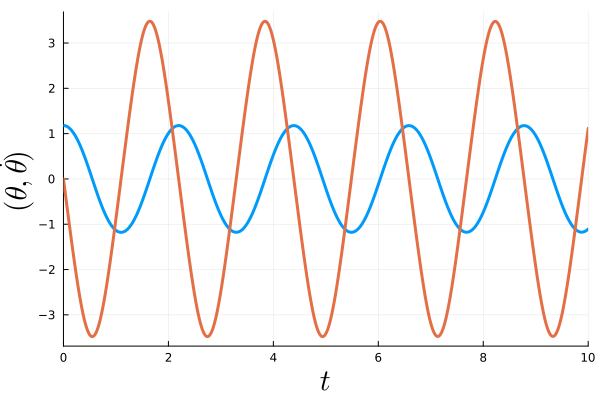
\includegraphics[width=0.6\columnwidth]{graphics/Chap09/PendulumSimulationChap09.png}
\end{center}

\Qed.

\bigskip

\begin{factColor}{2-Link Manipulator}{2LinkManipulator}

The base angle $q_1$ is an absolute angle, with its zero position aligned with the $x$-axis. The angle of the second link, $q_2$, is relative to the base (first) link. Hence, $q_2=0$ has the second link extending straight out from the base link. The angular velocities are denoted $dq_1$ and $dq_2$ in the code. Actuators have been placed at the base link and the second link, though we will not be using them in this Chapter. \\

\begin{lstlisting}[language=Julia,style=mystyle]
function dyn_mod_2LinkManipulator(q, dq)
# DYN_MOD_2LINKMANIPULATOR
# 2023-11-20 17:26:11
#
# Author: Grizzle
#
# Model NOTATION: D(q)ddq + C(q,dq)*dq + G(q) = B*tau 
# The Robot Equations: From Lagrange's Equations of Motion
#
g, L1, L2, m1, m2 = modelParameters()
#
# Variable names for the model
q1, q2 = q 
dq1, dq2 = dq
#
D = zeros(2, 2)
  D[1, 1] = L1^2*m1 + m2*(L1^2 + 2*L1*L2*cos(q2) + L2^2)
  D[1, 2] = L2*m2*(L1*cos(q2) + L2)
  D[2, 1] = L2*m2*(L1*cos(q2) + L2)
  D[2, 2] = L2^2*m2
#
C = zeros(2, 2)
  C[1, 1] = -L1*L2*dq2*m2*sin(q2)
  C[1, 2] = -L1*L2*m2*(dq1 + dq2)*sin(q2)
  C[2, 1] = L1*L2*dq1*m2*sin(q2)
#
G = zeros(2)
  G[1] = g*m2*(L1*cos(q1) + L2*cos(q1 + q2)) + L1*g*m1*cos(q1)
  G[2] = L2*g*m2*cos(q1 + q2)
#
B = zeros(2, 2)
  B[1, 1] = 1
  B[2, 2] = 1
#
JacG = zeros(2, 2)
  JacG[1, 1] = g*m2*(-L1*sin(q1) - L2*sin(q1 + q2)) - L1*g*m1*sin(q1)
  JacG[1, 2] = -L2*g*m2*sin(q1 + q2)
  JacG[2, 1] = -L2*g*m2*sin(q1 + q2)
  JacG[2, 2] = -L2*g*m2*sin(q1 + q2)
#
  return (D=D, C=C, G=G, B=B, JacG=JacG)
end
\end{lstlisting}

To bring the model into the workspace, use 

\begin{lstlisting}[language=Julia,style=mystyle]
# bring the model into the workspace for later use
include("dyn_mod_2LinkManipulator.jl") 
\end{lstlisting}    
\end{factColor}

\bigskip

\begin{example}
\label{ex:2LinkManipulatorFirstOrderODE}
A two-link manipulator model is given in Fact~\ref{thm:2LinkManipulator}, following the same angle convention as in Fig.~\ref{fig:RobotAbsoluteAngle}-(b). Express the model as a vector first-order ODE and provide a simulation with initial conditions 
\begin{align*}
    q_1(0) &= -\frac{3\pi}{8} \\
    q_2(0) & =0\\
    \dot{q}_1(0)&=0 \\
    \dot{q}_2(0) & = 0.
\end{align*}
\end{example}
\textbf{Solution:} Following the template given in Method~\ref{thm:SecondToFirstOrderODE}, we define
$$ x_1:= \left[ \begin{array}{c} q_1 \\
q_2
\end{array} \right] \text{ and } x_2:= \left[ \begin{array}{c} \dot{q}_1 \\
\dot{q}_2
\end{array} \right] .$$
We do not symbolically compute the inverse of the mass-inertia matrix because, in larger, more realistic models, it would make our simulation very slow. Hence, we write the model as
\begin{align*}
    \dot{x}_1 &= x_2 \\[1em]
    D(x_1) \dot{x}_2 & = -C(x_1, x_2)\cdot x_2 - G(x_1),
\end{align*}
and use the ``backslash'' operator to solve for $\dot{x}_2$. In code, it looks quite clean.

\begin{lstlisting}[language=Julia,style=mystyle]
# Import useful packages
using DifferentialEquations
using Plots 
using LaTeXStrings
using LinearAlgebra # for the backslash command
gr()

# 2-Link Manipulator Model
function modelParameters()
    g = 9.81
    L1 = 1.0
    L2 = 0.5
    m1 = 1.0
    m2 = 3.0
    return g, L1, L2, m1, m2
end

# bring the model into the workspace for later use
include("dyn_mod_2LinkManipulator.jl") 

# define the ODE dx/dt = f(x,t)
#
# the parameters are passed via modelParameters() in the
# function dyn_mod_2LinkManipulator(q, dq)
#
function f(x,~,t)
    n = floor(Int, length(x) / 2) # In Julia n/2 is a Float64
    q = x[1:n]
    dq = x[n+1:end]
    model = dyn_mod_2LinkManipulator(q, dq)
    dx1 = dq
    dx2 = (model.D) \ (-model.C*dq-model.G) # note the use of backslash
    dx=[dx1;dx2]
    return dx
end

# Set the initial condition as a vector
x0= [-3pi/8; 0.0; 0; 0]

# Set the time interval
T = (0.0, 5) 

# Setup the ODE problem with out-of-place function
# params removed 
problem = ODEProblem{false}(f, x0, T)

# solve the ODE problem using the Runge Kutta Tsitouras 5/4 Integrator
sol = solve(problem, Tsit5());

# plot the solution
p1 = plot(sol, lw=3, guidefont=20, xlabel=L"t", ylabel=L"(q_1, q_2, \dot{q}_1, \dot{q}_2)", 
    label=["q1" "q2" "dq1" "dq2"], legend=:topright)
\end{lstlisting}
\textbf{Output} 
The initial condition has the manipulator arm hanging downward like a pendulum ($q_1(0) = -\frac{\pi}{2}$ would be straight down). Consequently, $q_1$ oscillates similar to a single-link downward pointing pendulum, with one important change, some of the ``energy'' is transferred to the second link, which begins oscillating as well, even though it started in perfect alignment with the base link. Robot models with even two planar links have very complicated dynamics. Can you imagine the dynamics of a 3D bipedal robot, such as Cassie, with 14 links? Your answer should be an emphatic \textbf{\large NO!} 
\begin{center}
    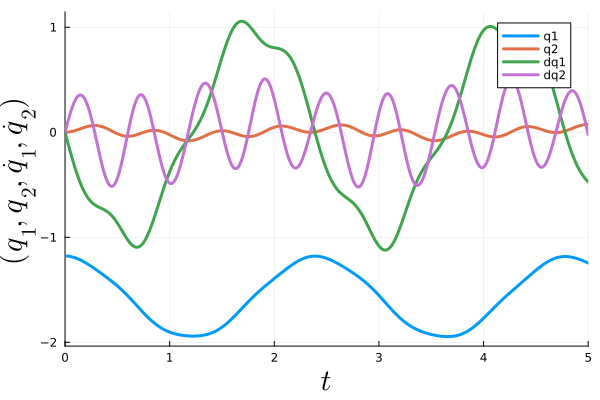
\includegraphics[width=0.6\columnwidth]{graphics/Chap09/2LinkManipulatorSimulationChap09.png}
\end{center}

\Qed.

\bigskip




\subsection{Solutions of First-order Vector ODEs}

\begin{tcolorbox}[colback=mylightblue, title = {\bf What is a Solution?}, breakable]
%%% Let $f:\real^n \to \real^n  \times [0, \infty)$ be a function.
\begin{definition}
\label{def:ODEsolution}
 A function,  $\bm{\varphi:[t_0, T) \to \mathbb{R}^n}$, $\bm{T > t_0}$, is a \textbf{solution} to the Ordinary Differential Equation (ODE) 
\begin{equation}
    \dot{x}(t) = f(x(t)), ~~x(t_0) = x_0,
\end{equation}
if 
 \begin{enumerate}
\renewcommand{\labelenumi}{(\alph{enumi})}
\setlength{\itemsep}{.2cm}
    \item $\varphi:[t_0, T) \to \real^n$ is continuous (meaning, each of its components is continuous);
    \item  $\varphi(t_0) = x_0$ (satisfies the initial condition); and
    \item for all $t \in (t_0, T)$, the derivative $\dot{\varphi}(t):=\frac{d}{dt} \varphi(t)$ exists and $\dot{\varphi}(t) - f(\varphi(t)) = 0_{n\times 1}$ (satisfies the differential equation).
\end{enumerate}
\end{definition}
\bigskip
\textbf{Note:} It is very common to drop the time variable and write the ODE as $\dot{x} = f(x), ~~x(t_0) = x_0$. The ``dot'' notation for the derivative indicates the dependence on time. 

\end{tcolorbox}

\bigskip

\begin{example} Show that for all constants $c>0$, 
$$
   \varphi_c(t) = 
    \begin{cases} 
      0 & \text{if } t < c, \\
      \frac{(t-c)^3}{27} & \text{if } t \ge c,
    \end{cases}
$$
is a solution to the differential equation $\dot{x} = \sqrt[3]{x^2}, ~x(0)=0$.
\end{example}
\textbf{Solution} We need to check the three conditions in Definition~\ref{def:ODEsolution}.
 \begin{enumerate}
\renewcommand{\labelenumi}{(\alph{enumi})}
\setlength{\itemsep}{.2cm}
    \item \textbf{Continuity:} The only point where continuity of $ \varphi_c(t)$ may be in doubt is $t=c$. We check, therefore, the two one-sided limits and compare them to the value of the function at $c$, viz,
    \begin{align*}
        \lim_{t \to c^-} \varphi_c(t) &=  \lim_{t \to c^-}~ 0 = 0~~(\text{the function is identically zero for }t< c) \\[1em]
        \lim_{t \to c^+} \varphi_c(t) &=   \lim_{t \to c^+}\frac{(t-c)^3}{27} = 0, ~~(\text{using the function's definition for }t> c) \\[1em]
        \varphi_c(t)~\bigg|_{t=c} &=  \frac{(t-c)^3}{27}~\bigg|_{t=c}  =0.
    \end{align*}
    Hence, the function is continuous at $c$ and therefore, at all points in its domain. 
    
    \item \textbf{Satisfies the Initial Condition:} $ 0= \frac{(t-c)^3}{27}~\bigg|_{t=c} = x_0$.

    \item \textbf{Satisfies the Differential Equation:} 
    \begin{itemize}
    \setlength{\itemsep}{.2cm}
        \item For $t < c$, $\varphi_c(t)$ is identically zero, and hence its derivative is also zero. Also, $(0)^{2/3}=0$. Hence, $\dot{\varphi_c}(t) - f(\varphi_c(t)) = 0$ for all $t<c$.
         \item For $t > c$, $\varphi_c(t) = \frac{(t-c)^3}{27}$, and hence by the Power Rule, 
         $$\frac{d}{dt} \varphi_c(t) = 3\frac{(t-c)^2}{27} = \frac{(t-c)^2}{3^2}= \left(\frac{(t-c)}{3} \right)^2.$$ 
         This takes care of the left side of the differential equation. Turning to the right side, 
         $$ \left(\varphi_c(t) \right)^{2/3} =  \left(\frac{(t-c)^3}{27} \right)^{2/3} = \left( \left(\frac{(t-c)}{3} \right)^3 \right)^{2/3} = \left(\frac{(t-c)}{3} \right)^2.$$
         Therefore, for all $t\neq c$, $\frac{d}{dt} \varphi_c(t)-\left(\varphi_c(t) \right)^{2/3} =0.$ \textbf{What about $\bm{t=c}$}, the point where the solution transitions from being identically zero to being a quadratic function of $t$? We need to evaluate the derivative at that point using left and right limits. It all works out, but we skip the details because there is a more general notion of a solution given in Chapter~\ref{sec:MoreGeneralSolutionODE} that obviates the calculation!
    \end{itemize}
    \end{enumerate}

\Qed. 



\bigskip

\subsection{Existence and Uniqueness of Solutions}
\label{sec:ExistenceUniquenessSolutionsODEs}

We recall from ROB 101 \textit{Computational Linear Algebra} that the \textbf{Euclidean norm} of a vector $x=\begin{bmatrix} x_1 & x_2  &  \cdots &  x_n  \end{bmatrix} $ is defined as
\begin{equation}
    \label{eq:DefEuclideanNorm}
    ||x||_2:=\sqrt{(x_1)^2 + (x_2)^2 + \cdots + (x_n)^2} = \sqrt{\sum_{i=1}^n (x_i)^2}.
\end{equation}
There are also other norms, such 
$$||x||_p:= \sqrt[\scalebox{1.0}{$p$}]{\sum_{i=1}^n (x_i)^p}, \quad 1 \le p < \infty \quad \text{and} \quad ||x||_{\rm max}:= \max_{1\le i \le n} |x_i|.$$

\bigskip

\begin{tcolorbox}[colback=mylightblue, title = {\bf Norm of a Matrix}, breakable]



\begin{definition}
 Let $A$ be an $n\times m$ matrix with entries $a_{ij}$. The \textbf{Euclidean norm} of $A$ is defined as 
\begin{equation}
    \label{eq:EuclideanNormA}
   ||A||_2:= \sqrt{\sum_{i=1}^n \sum_{j=1}^{m} (a_{ij})^2},
\end{equation}
the square root of the sum of all squared entries of $A$. This is the same as stacking the columns of $A$ into a large vector and applying the Euclidean norm to the resulting vector. 
\end{definition}

\bigskip 

\textbf{Note:} The Euclidean or 2-norm is the default norm in Julia obtained with \texttt{norm(A)}. There are many other ways to define norms on matrices. It is often easiest to use the following matrix norm
\begin{equation}
    \label{eq:MaxNormA}
   ||A||_\infty:= \max_{i,j} ~|a_{ij}|, 1 \le i, j \le n,
\end{equation}
which goes by the name \textbf{max norm} or the \textbf{infinity norm}.

\end{tcolorbox}

\bigskip


\begin{tcolorbox}[colback=mylightblue, title = {\bf Open Ball of Radius r}, breakable]
Open balls generalize to $\real^n$ the notion of open intervals in $\real$.\\

\begin{definition}
Let $x_0$ be a point in $\real^n$ and $r>0$ a constant. The \textbf{open ball of radius $\bm{r}$ centered about $\bm{x_0}$} is defined as 
\begin{equation}
    \label{eq:OpenBallRadiusLittleR}
   B_r(x_0):=\{ x\in \real^n~|~ ||x-x_0|| < r \}.
\end{equation}
The ball is called ``open'' because it does not include the boundary points where $||x-x_0||=r.$ 
\end{definition}

\bigskip \textbf{Note:} Open balls are used to specify when some property holds \textbf{locally} (meaning near a given point $x_0$), versus \textbf{globally} (meaning it holds for all $x\in \real^n$).

\end{tcolorbox}

\bigskip

\begin{example} Sketch the open balls about the origin for the 2-norm, 1-norm, and max-norm.    
\end{example}
\textbf{Solution:}

\bigskip
\begin{center}
    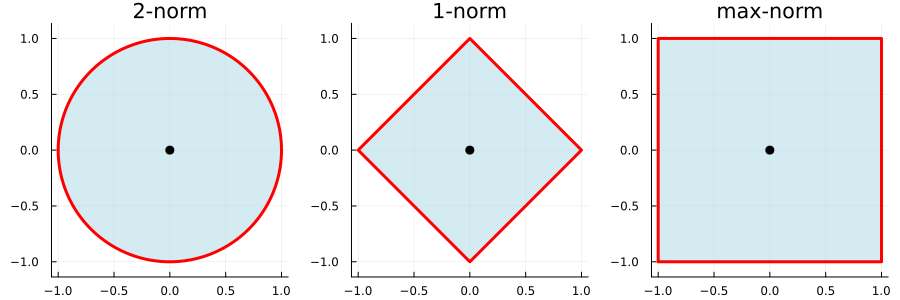
\includegraphics[width=0.95\columnwidth]{graphics/Chap09/UnitBalls.png}%
\end{center}

\bigskip
\begin{lstlisting}[language=Julia,style=mystyle]
using Plots

# Function to plot the unit ball for a given norm
function plot_unit_ball(norm_type::String)
    theta = range(0, stop=2π, length=1000) # parameter for the angle

    if norm_type == "2-norm"
        # Circle: x^2 + y^2 = 1
        x = cos.(theta)
        y = sin.(theta
    elseif norm_type == "1-norm"
        # Diamond: |x| + |y| = 1, simplified representation
        x = [0, 1, 0, -1, 0]
        y = [1, 0, -1, 0, 1]
    elseif norm_type == "max-norm"
        # Square: max(|x|, |y|) = 1, simplified representation
        x = [1, 1, -1, -1, 1]
        y = [1, -1, -1, 1, 1]
    else
        error("Unknown norm type")
    end

    plot(x, y, label="", aspect_ratio=:equal, title="$(norm_type)", fill=(0, 0.5, :lightblue), lw=3, color=:red)

end

# Plot unit balls for each norm
p1 = plot_unit_ball("2-norm")
p2 = plot_unit_ball("1-norm")
p3 = plot_unit_ball("max-norm")

# Display all plots in a single figure
pall= plot(p1, p2, p3, layout=(1, 3), size=(900, 300))
\end{lstlisting}
\textbf{Output} 
See the above plot.

\Qed

\bigskip


\begin{propColor}{Existence and Uniqueness of Solutions}{ExistenceUniquenessSolutionsODEs}

Consider a vector-valued ODE,
\begin{equation}
    \dot{x} = f(x), ~~x(t_0) = x_0 \in \real^n.
\end{equation}
\begin{enumerate}
\renewcommand{\labelenumi}{(\alph{enumi})}
\setlength{\itemsep}{.2cm}
    \item \textbf{(Local Existence and Uniqueness of a Solution)} If for some $r>0$, the Jacobian, $\frac{\partial f(x)}{\partial x}$, exists and is continuous for all $x\in B_r(x_0)$, then there exists $\delta>0$ such that the ODE has a unique solution on the interval $[t_0, t_0+\delta]$.
    
      \item \textbf{(Global Existence and Uniqueness of a Solution)} If there exists a constant $0 \le L< \infty$ such that, for all $x \in \real^n$, $||\frac{\partial f(x)}{\partial x}||\le L$, then the ODE has a unique solution on the unbounded interval $[t_0, \infty)$.
      \end{enumerate} 
\bigskip
\textbf{Note:}  It is often easier to check the condition for global existence and uniqueness with the max (aka, infinity norm) because it can be computed element by element; indeed,  $||\frac{\partial f(x)}{\partial x}||_\infty \le L$ for all $x \in \real^n$ if, and only if, $\displaystyle \sup_{x\in \real^n} |\frac{\partial f_i(x)}{\partial x_j}|\le L$.\\

\textbf{Note 2:} Most of the ODEs that appear in engineering practice satisfy the condition for local existence and uniqueness of a solution. However, the vector ODEs that model robots are typically quadratic in the angular velocities. Hence, their partial derivatives will be linear in the angular velocities, which means the global bound $||\frac{\partial f(x)}{\partial x}||\le L$ fails.   \\

\textbf{Note:} This topic is treated in great detail in Michigan's EECS 562 Nonlinear Systems and Control; see it for proofs.
\end{propColor}

\bigskip-

\begin{exercise} 
Apply Prop.~\ref{thm:ExistenceUniquenessSolutionsODEs} to the ODEs given in Fact~\ref{thm:ChuteModels}, Four Models of Chutes, to check for the local or global existence and uniqueness of their solutions. Comment on whether your conclusions match those of our previous calculations (of the solutions), or not. \\

For ease of reference, we repeat the ODEs here, rewritten slightly so that the left side only contains a derivative.
 \begin{enumerate}
\renewcommand{\labelenumi}{(\alph{enumi})}
\setlength{\itemsep}{.2cm}
\item \textbf{Model 1: Parallel Motion, Linear Drag:} $\frac{dv(t)}{dt} =  - \frac{\kappa}{m} v(t), ~~v(t_0) = v_0$.

\item \textbf{Model 2: Parallel Motion, Quadratic Drag:} $\frac{dv(t)}{dt} =  - \frac{\kappa}{m} v^2(t), ~~v(t_0) = v_0$.

\item \textbf{Model 3: Vertical Motion, Linear Drag:} $\frac{dv(t)}{dt} = - \frac{\kappa}{m} v(t)- g, ~~v(t_0) = v_0$.

\item \textbf{Model 4: Vertical Motion, Quadratic Drag:} $\frac{dv(t)}{dt} = \frac{\kappa}{m} v^2(t)-m, ~~v(t_0) = v_0$.
\end{enumerate}    
\end{exercise}
\textbf{Solutions:}

We use the generic notation, $\dot{v}=f(v)$, for each of the models.

\begin{enumerate}
\renewcommand{\labelenumi}{(\alph{enumi})}
\setlength{\itemsep}{.2cm}
\item  $\dot{v} =  - \frac{\kappa}{m} v, ~~v(t_0) = v_0$. \quad \Ans~~\textbf{Prop.~\ref{thm:ExistenceUniquenessSolutionsODEs} implies global existence and uniqueness of solutions.} \\

We have $f(v) =  - \frac{\kappa}{m} v$. Therefore, $\frac{df(v)}{dv} = - \frac{\kappa}{m} $ and $|\frac{df(v)}{dv}| =|- \frac{\kappa}{m} | = \frac{\kappa}{m}$ is finite for all $v\in \real$. Therefore, 
Prop.~\ref{thm:ExistenceUniquenessSolutionsODEs} implies a solution exists and is unique for all $t>t_0$ and all $v_0 \in \real$.\\

Comparison to our calculations in Example~\ref{eq:ChuteODE01}: we obtained a globally defined solution but had no means to check uniqueness. 

\item $\dot{v} =  - \frac{\kappa}{m} v^2, ~~v(t_0) = v_0$. \Ans~ \textbf{Prop.~\ref{thm:ExistenceUniquenessSolutionsODEs} implies local existence and uniqueness of solutions.} \\

We have $f(v) =  - \frac{\kappa}{m} v^2$. Therefore, $\frac{df(v)}{dv} = - 2 \frac{\kappa}{m} v$. The magnitude of the Jacobian, $|\frac{df(v)}{dv}|$, is finite on any open ball $B_r(v_0)$, $0 < r < \infty$, but grows unbounded as $|v| \to \infty$. Therefore, 
Prop.~\ref{thm:ExistenceUniquenessSolutionsODEs} implies the existence of $\delta>0$ such that a solution exists and is unique for all $t \in[t_0, t_0+\delta]$ and all $v_0 \in \real$, but does not imply global existence and uniqueness.\\

Comparison to our calculations in Example~\ref{eq:ChuteODE02}: we obtained a globally defined solution, even though the sufficient conditions of the Proposition only guaranteed a local solution. At the time we solved this problem, we had no means to check uniqueness. \\

\textbf{Note:} If we ``flip the sign'' on the ODE to $\frac{dv}{dt} =  \frac{\kappa}{m} v^2$, then $|\frac{df(v)}{dv}| =2 \frac{\kappa}{m} | v|$ as before, again implying only local existence and uniqueness of solutions. This time, the method of separation of variables gives
$$v(t) = \frac{v_0}{1 - v_0  \frac{\kappa}{m} (t-t_0)}, $$
which blows up at $t=t_0 + \frac{m}{\kappa \cdot v_0}$ because the denominator vanishes. By flipping the sign in front of the equation, we go from one with a globally defined solution to one that blows up in finite time. The test given in Prop.~\ref{thm:ExistenceUniquenessSolutionsODEs} is based on the norm of the Jacobian of the right side of the equation, and norms are invariant under sign changes. 

\item $\dot{v} = - \frac{\kappa}{m} v(t)- g, ~~v(t_0) = v_0$. \Ans~ \textbf{Prop.~\ref{thm:ExistenceUniquenessSolutionsODEs} implies global existence and uniqueness of solutions.} \\

We have $f(v) =  - \frac{\kappa}{m} v - g$. Therefore, $\frac{df(v)}{dv} = - \frac{\kappa}{m} $ and $|\frac{df(v)}{dv}| =|- \frac{\kappa}{m} | = \frac{\kappa}{m} < \infty$. Therefore, 
Prop.~\ref{thm:ExistenceUniquenessSolutionsODEs} implies a solution exists and is unique for all $t>t_0$ and all $v_0 \in \real$.\\

Comparison to our calculations in Example~\ref{eq:ChuteODE03}: we obtained a globally defined solution but had no means to check uniqueness. 

\item $\dot{v} = \frac{\kappa}{m} v^2(t)-g, ~~v(t_0) = v_0$.  \Ans~ \textbf{Prop.~\ref{thm:ExistenceUniquenessSolutionsODEs} implies local existence and uniqueness of solutions.} \\

We have $f(v) =  - \frac{\kappa}{m} v^2 -g$. Therefore, $\frac{df(v)}{dv} = - 2 \frac{\kappa}{m} v$ and the magnitude of the Jacobian, $|\frac{df(v)}{dv}|$, is finite on any open ball $B_r(v_0)$, $0 < r < \infty$, but grows unbounded as $|v| \to \infty$. Therefore, Prop.~\ref{thm:ExistenceUniquenessSolutionsODEs} implies the existence of $\delta>0$ such that a solution exists and is unique for all $t \in[t_0, t_0+\delta]$ and all $v_0 \in \real$.\\

Comparison to our calculations in Example~\ref{ex:ChuteODE04}: we were unable to obtain an analytical solution. Our numerical calculations showed the existence of a solution over an adequately large time domain. Our previous work provided no means to check uniqueness. \\
\end{enumerate} 
\Qed

\bigskip

\begin{exercise} Revisit the ODE in \eqref{eq:ODEwithNonuniqueSolutions}, where we produced an infinite number of solutions (non-uniqueness on steroids),
$$
    \dot{x} = \left(x\right)^{2/3}, ~x(0)=0.
$$
In what manner does it fail the conditions in Prop.~\ref{thm:ExistenceUniquenessSolutionsODEs}?    
\end{exercise}
\textbf{Solution:}
The discussion in Chapter~\ref{sec:ODEwithInfiniteSolutions} gave us a heads up on the issue, but we'll continue as if that had not happened! Define $f(x):=x^{2/3}$. 
Prop.~\ref{thm:ExistenceUniquenessSolutionsODEs} tells us to evaluate 
$$ \frac{df(x)}{dx} =  \frac{d}{dx} \left( x^{2/3} \right) = \frac{2}{3}x^{ -\frac{1}{3}} = \frac{2}{3} \frac{1}{ \sqrt[3]{x}},$$
which blows up at the initial condition, $x_0 = 0$. Hence, none of the conditions of Prop.~\ref{thm:ExistenceUniquenessSolutionsODEs} are met, so it has nothing to say about the solutions of the ODE.

\Qed


\bigskip

\begin{exercise} Differential equations are pivotal in modeling epidemics, showcasing how susceptible individuals ($x_1(t)$) and infectious individuals ($x_2(t)$) interact over time. The transition of susceptibles to infectious hinges on direct contact, captured by $\beta x_1 x_2$, where $\beta$ denotes the infection rate. Furthermore, infectious individuals either recover, gaining immunity, or succumb to the illness, at a rate proportional to $\gamma x_2$, with $\gamma$ reflecting the disease's time constant. Vaccination efforts, represented by a rate $u$, can reduce the number of susceptible individuals, illustrating the model's capacity to inform public health interventions.

The dynamics are governed by two differential equations,
\begin{align}
\frac{d x_1}{dt} &= -\beta x_1 x_2 - u, \\
\frac{d x_2}{dt} &= \beta x_1 x_2 - \gamma x_2,
\end{align}
where, $x_1(t)$ and $x_2(t)$ represent susceptible and infectious individuals, respectively, integrating how the disease spreads and recedes within the community. Parameters $\beta$ and $\gamma$ quantify infection and recovery rates, pivotal in understanding the epidemic's trajectory. This model, by delineating interaction dynamics, aids in predicting and mitigating disease spread, underscoring the value of mathematical approaches in public health. \\

The epidemic model depends on two parameters $\beta >0$ and $\gamma>0$, and two states, $x_1$ and $x_2$. Assuming $u$ is constant, 
\begin{enumerate}
\renewcommand{\labelenumi}{(\alph{enumi})}
 \setlength{\itemsep}{.2cm}
    \item determine if local existence and uniqueness of solutions can be guaranteed for all $x_1\ge 0$, $x_2\ge 0$; moreover, 
    \item determine if global existence and uniqueness of solutions can be guaranteed.
\end{enumerate}

\end{exercise}
\textbf{Solution:}

Define $f(x) := \left[ \begin{array}{l}  -\beta x_1 x_2 - u \\ \beta x_1 x_2 - \gamma x_2 \end{array}\right]$.\\

\begin{enumerate}
\renewcommand{\labelenumi}{(\alph{enumi})}
 \setlength{\itemsep}{.2cm}
    \item Local existence and uniqueness of solutions: \Ans \quad Yes.\\

The Jacobian,
    $$ \frac{ \partial f(x)}{\partial x}= \left[ \begin{array}{cc}  -\beta x_2  & -\beta x_1 \\ \beta x_2 &  \beta x_1 - \gamma \end{array}\right],$$
    is continuous everywhere, and hence, the condition for local existence and uniqueness is met for all $x_1\ge 0$, $x_2\ge 0$. 

    
    \item Global existence and uniqueness of solutions: \Ans \quad No.\\

We use the max norm and note immediately that the $(1,1)$ element of the Jacobian satisfies $ \displaystyle \sup_{x_1\ge 0, x_2\ge 0} \Big|\frac{f_1(x)}{\partial x_1}\Big| = \sup_{x_2\ge 0} |-\beta x_2| = \infty$, and hence 
$$ \|\frac{\partial f(x)}{\partial x}  \|_\infty > L$$
for all finite $L$.\\

\textbf{Note:} Does this mean that solutions definitely blow up? No! Our calculations mean that we cannot prove global existence and uniqueness with the elementary means treated in the textbook. More powerful methods from Michigan's EECS 560 \textit{Nonlinear Systems and Control} must be employed. Consider $V(x_1, x_2):= x_1 + x_2$, the total population of individuals. Then an easy calculation shows that $\frac{d}{dt}V(x_1, x_2) = \dot{x}_1 + \dot{x}_2 = -u - \gamma x_2 \le 0$ when $u\ge 0$. Hence, the total population remains bounded, ruling out a finite escape time, and ensuring global existence and uniqueness of solutions.     
\end{enumerate}
\Qed

\bigskip

\emstat{
\textbf{ODE Examples from a Plethora of Engineering Domains:} The (free) textbook, \href{https://www.dropbox.com/scl/fi/leg5vkbkyjsi4bye9gmb4/McClamrochStateModelsDynSys.pdf?rlkey=yn1umtkys6griqpfqi4ekwa2k&dl=0}{State Models and Dynamical Systems} by Prof. Emeritus N. Harris McClamroch, aims to enhance undergraduate students' understanding of dynamic physical processes through applied mathematics and systems theory. It is written assuming that readers have a background in calculus, differential equations, Laplace transforms, physics, mechanics, and circuits. The book introduces mathematical systems theory, using case studies to clarify complex concepts.
}

\bigskip

\begin{example} Show that the condition for global existence and uniqueness fails for the 2-link manipulator model from Fact~\ref{thm:2LinkManipulator} and Example~\ref{ex:2LinkManipulatorFirstOrderODE}.    
\end{example}
\solution 
Let $\dot{x}=f(x)$ be the state variable model as expressed in Example~\ref{ex:2LinkManipulatorFirstOrderODE}, after inverting $D(q)$. Using symbolic computations, we compute
$$J_{33}:=\frac{\partial f_3(q_1, q_2, \dot{q}_1, \dot{q}_2)}{\partial \dot{q}_1} = \alpha(q_1, q_2) \dot{q}_1 + \beta(q_1, q_2) \dot{q}_2,$$
where
\begin{align*}
\alpha(q_1, q_2) & =  \frac{-4 \cdot m_2 \cdot (L_2 + L_1 \cdot \cos(q_2)) \cdot \sin(q_2)}{L_1 \cdot (-2 \cdot m_1 - m_2 + m_2 \cdot \cos(2 \cdot q2))} \\[1em]
%
\beta(q_1, q_2) & = 
    \frac{-4 \cdot L_2 \cdot m_2 \cdot \sin(q_2)}{-2 \cdot L_1 \cdot m_1 - L_1 \cdot m_2 + L_1 \cdot m_2 \cdot \cos(2 \cdot q_2)}
\end{align*}
Hence, for $q_2 \neq \pm \frac{\pi}{2}$ (modulo $\pi)$, $\alpha(q_1, q_2) \neq 0$ and then 
$$ \sup_{\dot{q}_1} J_{33} = \infty,$$
and therefore $||\frac{\partial f}{\partial x}||$ cannot be uniformly bounded. More generally, if a robot model has two or more revolute joints, then it is pretty much guaranteed to fail the test we have given for global existence and uniqueness of solutions for the same reason underlined here: at least one component of the Jacobian will be linear (affine) in at least one component of the generalized velocity coordinates. 
\Qed


\subsection{(Optional Read:) More General Notion of a Solution}
\label{sec:MoreGeneralSolutionODE}

Consider a rather general vector ODE that may even depend explicitly upon time,
\begin{equation}
\label{eq:GeneralODE}
    \dot{x}(t) = f(x(t), t), ~~x(t_0) = x_0.
\end{equation}
An ODE is an equation relating $x(t)$ and its derivative, $\dot{x}(t)$. We know that $x(t)$ is always an antiderivative of $\dot{x}(t)$. The First Fundamental Theorem of Calculus\footnote{While the Fundamental Theorems of Calculus apply to scalar-valued functions of a single variable, we can apply them to each component of a vector-valued function of a single variable, $t$.} 
%
states that if $x(t)$ is an antiderivative of $x'(t)$ ($ x'(t) = \dot{x}(t)=\frac{d}{dt} x(t)$ depending on the notation of the moment), the two functions must be related by 
\begin{equation}
\label{eq:FirstFundThmofCalculus}
    x(t) = x(t_0) + \int_{t_0}^t  x'(\tau) \, d \tau~~~~~ \textbf{and}~~~~~ \frac{d}{dt} \left( x(t_0) + \int_{t_0}^t  x'(\tau) \, d \tau \right) =   x'(t).
\end{equation}
We can then plug \eqref{eq:GeneralODE} into \eqref{eq:FirstFundThmofCalculus} and obtain that $x(t)$, $f(x(t), t)$, $x'(t)$ and $\dot{x}(t)$ are related by
\begin{equation}
\label{eq:FirstFundThmofCalculusMeetsODE}
    x(t) = x(t_0) + \int_{t_0}^t \underbrace{f(x(\tau), \tau)}_{x'(\tau)} \, d \tau~~~~~ \textbf{and}~~~~~ \frac{d}{dt} \left( x(t_0) + \int_{t_0}^t  \underbrace{f(x(\tau), \tau)}_{x'(\tau)} \, d \tau \right) =   \underbrace{\dot{x}(t)}_{x'(t)}.
\end{equation}
Therefore, the equation 
\begin{equation}
\label{eq:FirstFundThmofCalculusForODEs}
x(t) = x_0 + \int_{t_0}^t f(x(\tau), \tau) \, d \tau,
\end{equation}
relating $x(t)$ and an indefinite integral depending upon $x(t)$, is equivalent to the ODE \eqref{eq:GeneralODE}, relating $x(t)$ and its derivative $\dot{x}(t)$. The interesting property of \eqref{eq:FirstFundThmofCalculusForODEs} is that the derivative of $x(t)$ does not show up explicitly, and hence functions that are only ``piecewise differentiable'', instead of differentiable everywhere, can also be solutions of the ODE \eqref{eq:GeneralODE}. \textcolor{blue}{\bf We care about this as engineers because, when we design feedback controllers for a system (e.g., a robot), we often send command signals to the closed-loop system that are only piecewise continuous; that is, the command signals have jumps in them.} \textcolor{black}{\bf Engineer to Robot: ``Move forward at 1 m/s.''} \textcolor{red}{\bf The engineer sees an obstacle. Engineer screams to Robot: ``Stop! Stop immediately...'' as they slam the joystick in full reverse!} \textcolor{black}{\bf As engineers, we'd like to know that a solution to the differential equations that govern our robot does not cease to make sense as soon as we send a very abrupt (non-differentiable) change in the command signal.} 



\section{Linear Systems of ODEs}


When the right side of the ODE $\dot{x} = f(x)$ is linear in $x$, one would hope that it is simpler to compute analytical solutions and/or understand various properties of the solution. This is indeed the case and motivates the present section.

\bigskip

\begin{tcolorbox}[colback=mylightblue, title = {\bf Homogeneous Linear Systems}, breakable]

\begin{definition}
For $A$ an $n \times n$ real matrix, 
\begin{equation}
    \label{eq:HomogeneousLinearSystem}
  \dot{x} = A x, ~x(t_0) = x_0
\end{equation}
is called a \textbf{homogeneous linear system of differential equations}.
\end{definition}
\bigskip
\textbf{Notes:} By Prop.~\ref{thm:MatrixVectorCalculusFormulas}-(a), $\frac{\partial}{\partial x} \left( Ax \right) = A$, which is independent of $x$. Hence, Prop.~\ref{thm:ExistenceUniquenessSolutionsODEs}-(b) implies the global existence and uniqueness of solutions. In other words, for all $x_0\in \real^n$, $t_0\in \real$, there exists a solution on $[t_0, \infty)$ and the solution is unique.  
\end{tcolorbox}

\subsection{Examples from Circuits and Mechanics}

\bigskip

\begin{example} 
\label{ex:RLCcircuit}
Using Kirchoff's Laws for linear RLC circuits, derive a differential equation model for the given circuit. The basics of Kirchoff's laws will be given in the solution. For more details, you can see \href{https://youtu.be/6F_rmZ1nXFQ}{Kirchhoff's Voltage Law - KVL Circuits, Loop Rule \& Ohm's Law - Series Circuits, Physics} and \href{https://youtu.be/2Zu3ppq3n8I}{Kirchhoff's Law, Junction \& Loop Rule, Ohm's Law - KCL \& KVL Circuit Analysis - Physics}, both by the Organic Chemistry Tutor.

\begin{center}

\begin{circuitikz}
    \draw (0,0)
    to[V,v=$V_S$] (0,2) % Voltage source
    to[R, l=$R$] (2,2) % Resistor
    to[L, l=$L$] (4,2) % Inductor
    to[C, l=$C$] (4,0) % Capacitor
    -- (0,0);
    \draw[->,>=stealth] (2,0.1) arc (270:0:0.8);
    \draw (2.0,0.5) node[anchor=east] {$i$};
\end{circuitikz}
    
\end{center}

\jwg{Need to add signs to the circuit model. I should have $-V_S + V_R + V_L + V_C = 0$ when all is said and done.}
\end{example}
\textbf{Solution:} $V_s$ is a voltage source, which could be a battery or something more capable, such as a power supply. $R$ denotes a resistor, $L$ an inductor, and $C$ a capacitor. The loop denotes the reference direction for the current flowing through the circuit, $i(t)$. \textbf{Kirchoff's Voltage Law} says that the sum of the voltages around any loop must equal zero. This gives us
\begin{equation}
\label{eq:KVL}
    V_S + V_R + V_L + V_C = 0.
\end{equation}
So far, there are no derivatives in sight! The \textbf{constitutive relations} for the three circuit elements are 
\begin{equation}
\label{eq:ConstiutiveRelationsRLC}
    \begin{aligned}
        V_R & = R \cdot i\\
        V_L & = L \frac{d i}{dt} \\
        i & = C \frac{dV_C}{dt},
    \end{aligned}
\end{equation}
which, in plain words, means that the voltage across a resistor is proportional to the current flowing through it, the voltage across the inductor is proportional to the time derivative of the current, and the current through the capacitor is proportional to the time derivative of the voltage across the capacitor, denoted here as $ \frac{dV_c}{dt}$. Now that we have derivatives, we can build an ODE model. The rest is ``algebra''.\\

If we assign state variables by
\begin{equation}
\label{eq:StatesRLCCircuit}
    \begin{aligned}
        x_1 &:= V_C \\
        x_2 & := i,
    \end{aligned}
\end{equation}
then, from line three of \eqref{eq:ConstiutiveRelationsRLC}, we have 
\begin{equation}
\label{eq:RLCequationOne}
    \dot{x}_1 = \frac{1}{C} x_2.
\end{equation}
The equation for $ \dot{x}_2$ comes from Kirchoff's Voltage Law as given by \eqref{eq:KVL} in tandem with lines one and two of \eqref{eq:ConstiutiveRelationsRLC}. Indeed, from \eqref{eq:KVL}, we obtain
$$ V_L = -V_s - V_R - V_C,$$
which from \eqref{eq:ConstiutiveRelationsRLC} gives,
$$  L \frac{d i}{dt} = -V_s - r \cdot i - V_C.$$
From the definition of the state variables in \eqref{eq:StatesRLCCircuit}, we obtain
\begin{equation}
\label{eq:RLCequationTwo}
\begin{aligned}
     L \dot{x}_2 &= - Cx_1 -R x_2 -V_s \\
     &\Updownarrow \\
    \dot{x}_2 &= - \frac{C}{L}x_1 -\frac{R}{L} x_2 - \frac{1}{L}V_S . 
\end{aligned}
\end{equation}
Combining \eqref{eq:RLCequationOne} and \eqref{eq:RLCequationTwo} gives
\begin{equation}
\label{eq:InhomogeneousRLCwithVoltageSource}
\left[ \begin{array}{c} \dot{x}_1  \\ \dot{x}_2 \end{array} \right] = \left[ \begin{array}{cc} 0 & \frac{1}{C}\\- \frac{C}{L} & -\frac{R}{L} \end{array}\right] \left[ \begin{array}{c} x_1  \\ x_2 \end{array}\right] + \left[ \begin{array}{c} 0  \\  \frac{1}{L} \end{array}\right] V_s.
\end{equation}
Equation \eqref{eq:InhomogeneousRLCwithVoltageSource} is an inhomogeneous system of linear equations due to the voltage source, $V_s$. If we assume $V_s\equiv 0$, we obtain 
\begin{equation}
\label{eq:HomogeneousRLCwithVoltageSource}
\left[ \begin{array}{c} \dot{x}_1  \\ \dot{x}_2 \end{array} \right] = \left[ \begin{array}{cc} 0 & \frac{1}{C}\\- \frac{C}{L} & -\frac{R}{L} \end{array}\right] \left[ \begin{array}{c} x_1  \\ x_2 \end{array}\right].
\end{equation}
The initial conditions for \eqref{eq:HomogeneousRLCwithVoltageSource} come from the initial voltage across the capacitor and the initial current through the inductor.
\Qed

\bigskip

\textcolor{blue}{\bf Hence, RLC circuits give rise to linear systems of ODEs. In a similar manner, mechanical systems without ``rotating elements'' (aka, only have elements that move in a straight line) ``mostly'' give rise also to linear systems of ODEs when stiction and dead zones are ignored.}

\bigskip

\begin{example} 
\label{ex:MassSpringDamperNoGravity}
Using either Newton's Laws or Lagrange's Equations of Motion, derive a linear differential equation model for the mass-spring-damper system below. 

\begin{center}
\begin{tikzpicture}

% Wall
\draw[pattern=north east lines] (-1,-0.5) rectangle (0,1.5);
\draw[thick] (0,-0.5) -- (0,1.5);

% Damper
\draw[thick] (0,1) -- (2,1);
\draw[thick,decoration={markings,  
mark connection node=dmp,
mark=at position 0.5 with 
{
    \node (dmp) [thick,inner sep=0pt,transform shape,rotate=-90,minimum width=15pt,minimum height=3pt,draw=none] {};
}
}, decorate] (0,1) -- (2,1);
\draw[thick] (dmp.north east) -- (dmp.north west);
\draw[thick] (dmp.south east) -- (dmp.south west);

% Spring
\draw[decoration={aspect=0.3, segment length=3mm, amplitude=3mm,coil},decorate] (0,0) -- (2,0); 

% Mass
\draw[fill=black!20] (2,0.5) rectangle (3,-0.5);
\draw (2.5,0) node {$m$};

% Connecting Damper to Mass
\draw[thick] (2,1) -- (2.5,1) -- (2.5,0.5);

% Labels
\draw (1,-1.0) node[above] {Spring};
\draw (1,1.5) node[above] {Damper};
\draw (-1.1,0.5) node[left] {Wall};
\draw (3.1,0.0) node[right] {Mass};

\end{tikzpicture}
\end{center}    
\end{example}
\textbf{Solution:} We assume the wall is immovable and let $x$ be the distance of the mass from the wall, with positions to the right of the wall being positive. The velocity of the mass is denoted $\dot{x}$, and its Kinetic Energy is $\frac{1}{2} m \dot{x}^2$. Let the rest position of the spring be $x_s$ (the position of the spring when it is neither compressed nor stretched). The Potential Energy of the spring is then $\frac{1}{2} k \left(x-x_s \right)^2$. The effect of the linear damper, $-b \dot{x}$, must be placed in $\Gamma$. With these assumptions, Lagrange's equations become
\begin{equation}
    \begin{aligned}
        &L(x, \dot{x})= \frac{1}{2} m \dot{x}^2 - \frac{1}{2} k \left(x-x_s \right)^2 \\[1em]
       & \frac{d}{dt}\frac{\partial L}{\partial \dot{x}}- \frac{\partial L}{\partial x} = \Gamma,
    \end{aligned}
\end{equation}
where $k$ is the spring constant, $b$ is the damping coefficient, and $\Gamma =  -b \dot{x}$. Computing the indicated derivatives gives
\begin{equation}
\begin{aligned}
    \frac{d}{dt}\left(m  \dot{x} \right) + k\left( x-x_s\right) &= -b \dot{x} \\
 \Updownarrow \hspace{1.5cm}   &  \\
     m \ddot{x} + b \dot{x} + k\left( x-x_s\right) &= 0.
\end{aligned}     
\end{equation}
Assigning state variables as
\begin{equation}
\label{eq:StatesMassSpringDamper}
    \begin{aligned}
        x_1 &:= x - x_s \\
        x_2 & := \dot{x},
    \end{aligned}
\end{equation}
gives the relationships
\begin{equation}
\label{eq:HomogeneousMassSpringDamperTwo}
\begin{aligned}
   \dot{x}_1 &= x_2\\
   m \dot{x}_2 &= -k x_1 - b x_2. 
\end{aligned}
\end{equation}
Therefore, the linear homogeneous model is
\begin{equation}
\label{eq:HomogeneousMassSpringDamperThree}
\left[ \begin{array}{c} \dot{x}_1  \\ \dot{x}_2 \end{array} \right] = \left[ \begin{array}{cc} 0 & 1\\- \frac{k}{m} & -\frac{b}{m} \end{array}\right] \left[ \begin{array}{c} x_1  \\ x_2 \end{array}\right].
\end{equation}
The initial conditions for \eqref{eq:HomogeneousMassSpringDamperThree} come from the initial position of the mass (relative to the rest position of the spring) and the initial velocity of the mass.

\Qed

\subsection{Expressing Higher-order Linear ODEs in First-order Form}

In Definition~\ref{def:nthOrderODE}, we introduced the notion of ``higher order ODES of a single variable'', where the linear model takes the form
$$
   y^{(n)} + a_{n-1} y^{(n-1)} + a_{n-2} y^{(n-2)} +  \cdots +  a_1 \dot{y} + a_0 y = 0.
$$
Such models can be written as a vector first-order system of linear ODEs by assigning state variables as follows
\begin{equation}
    \left[ \begin{array}{c} x_1 \\ x_2 \\ \vdots\\ x_{n-1} \\ x_n \end{array} \right] =  \left[ \begin{array}{c} y \\ \dot{y} \\ \vdots\\ y^{(n-2)} \\ y^{(n-1)} \end{array} \right],
\end{equation}
 so that
 \begin{equation}
    \frac{d}{dt} \left[ \begin{array}{c} x_1 \\ x_2 \\ \vdots\\ x_{n-1} \\ x_n \end{array} \right] =  \left[ \begin{array}{c} \dot{y} \\ \ddot{y} \\ \vdots\\ y^{(n-1)}  \\ y^{(n)} \end{array} \right] = \left[ \begin{array}{c} x_2\\ x_3 \\ \vdots\\ x_n  \\ -a_0 x_1 - a_1 x_2 - \cdots - a_{n-1}x_n\end{array} \right].
\end{equation}
In matrix form, the system of ODEs becomes 
\begin{equation}
    \dot{x} = \underbrace{ \left[ \begin{array}{ccccccc} 
    0 & 1 & 0 & 0 &\cdots & 0  & 0 \\
     0 & 0 & 1 & 0 &\cdots & 0  & 0 \\
    0 & 0 & 0 & 1 &\cdots & 0  & 0 \\
    \vdots & \vdots & \vdots & \vdots &\ddots & 0  & 0 \\
 0 & 0 & 0 & 0 &\ddots & 1  & 0 \\
 0 & 0 & 0 & 0 &\ddots  & 0 & 1 \\
     -a_0 & -a_1 & -a_2 & -a_3 &\cdots& -a_{n-2} & -a_{n-1} \\
    \end{array} \right]}_{A} \cdot x.
\end{equation}

\bigskip

\begin{example} Rewrite the second-order linear mass-spring-damper model,
$$ m \ddot{x} + b \dot{x} + k\left( x-x_s\right) = 0,$$
as a linear state-variable model.    
\end{example}
\textbf{Solutions:}
We first solve for $ \ddot{x}$, yielding
$$ \ddot{x} = - \frac{k}{m} \left( x-x_s\right) -\frac{b}{m} \dot{x}.$$
Assigning state variables as
\begin{align*}
            x_1 &:= x - x_s \\
        x_2 & := \dot{x},
\end{align*}
gives the relationships
\begin{align*}
   \dot{x}_1 &= x_2\\
 \dot{x}_2 &= -\frac{k}{m} x_1 - \frac{b}{m} x_2. 
\end{align*}
Therefore, the linear homogeneous model is
$$
\left[ \begin{array}{c} \dot{x}_1  \\ \dot{x}_2 \end{array} \right] = \left[ \begin{array}{cc} 0 & 1\\- \frac{k}{m} & -\frac{b}{m} \end{array}\right] \left[ \begin{array}{c} x_1  \\ x_2 \end{array}\right],
$$
just as we derived in Example~\ref{ex:MassSpringDamperNoGravity}.

\Qed

\subsection{Linearization of Nonlinear ODE Models}

In engineering practice, linear models predominantly arise from local approximations of nonlinear models around equilibrium points, that is, initial conditions where the system remains constant unless disturbed. The utility of linear approximations might seem counterintuitive, given our ability to compute solutions for complex nonlinear models numerically. However, often, the real challenge lies not in modeling systems but in modifying their behavior. Consider the example of a Segway: while creating and simulating its nonlinear dynamical model is straightforward, designing a feedback control system to maintain its balance is far more complex. Here, linearization becomes invaluable. By simplifying a nonlinear system to its linear counterpart around an equilibrium point, we gain a more manageable framework. This linear approximation facilitates the use of well-developed linear control techniques like PID control and state-space analysis, offering crucial insights into the system's stability and response near the equilibrium. Such simplifications are essential for effective control system design and analysis despite being local approximations that may not fully capture the system's behavior in more extreme conditions.

\begin{tcolorbox}[colback=mylightblue, title = {\bf Equilibrium Points}, breakable]

\begin{definition} 
   \label{def:equilibriumPoint}
A vector $x_e \in \real^n$ is an \textbf{equilibrium point} of the differential equation $\dot{x} = f(x)$ if $f(x_e) = 0_{n \times 1}$. 
Equivalently, $x_e$ is an equilibrium point if the constant function $\varphi(t, t_0, x_e):=x_e$ is a solution of the ODE. \\
\end{definition}
 \vspace*{.1cm}
\textbf{Notes:} 
\begin{itemize}
    \item In simple terms, equilibrium points are initial conditions from which the solution of the ODE does not change; it remains constant and equal to the initial condition. For example, if a pendulum is initialized at rest in the downward hanging position, it stays there!
    \item Determining points $x_e$ such that $f(x_e)=0$ is a root finding problem; hence, Newton-Raphson is an effective means for finding equilibrium points in cases where the physics of a problem does not make them obvious.
    \item For a linear ODE, $\dot{x} = Ax$, $x_e$ is an equilibrium point if, and only if, $x_e \in \nullspace(A)$. In particular, for a linear ODE, the origin is always an equilibrium point.
\end{itemize}
\end{tcolorbox}

 \bigskip

\begin{example} 
\label{ex:equilibriumPoints}
Find equilibrium points for the following ordinary differential equations,  
 \begin{enumerate}
\renewcommand{\labelenumi}{(\alph{enumi})}
\setlength{\itemsep}{.2cm}
    \item $\frac{dv(t)}{dt} =   \frac{\kappa}{m} v^2(t) - g$ (parachutist with nonlinear drag, from Example~\ref{ex:ChuteODE04}).
    \item $\left[ \begin{array}{c} \dot{x}_1 \\ \dot{x}_2 \end{array} \right]= \left[\begin{array}{c} x_2 \\  -\frac{g}{L}  \cdot \sin(x_1)\end{array} \right]$ (pendulum model from Examples~\ref{ex:PendulumModel} and \ref{ex:PendulumModelTake2}).
    \item $ \left[ \begin{array}{c} \dot{x}_1 \\ \dot{x}_2 \end{array} \right] = \left[\begin{array}{c} x_2 \\-D^{-1}(x_1) \cdot \left[ C(x_1, x_2) \cdot x_2 + G(x_1)\right] \end{array} \right] $ (the robot equations from Method~\ref{thm:SecondToFirstOrderODE}).
\end{enumerate} 
\end{example}
\textbf{Solutions:}
 \begin{enumerate}
\renewcommand{\labelenumi}{(\alph{enumi})}
\setlength{\itemsep}{.8cm}
    \item $\dot{v} =   \frac{\kappa}{m} v^2 - g$ \quad \Ans $v_e = -\sqrt{ \frac{m\,g}{\kappa} }.$ \\

We set the right side to zero and solve for $v$. This gives $v^2 =  \frac{m\,g}{\kappa}$. Solving for $v$ gives $v_e = \pm \sqrt{ \frac{m\,g}{\kappa} }$. However, only the negative velocity makes sense because the parachutist is not falling upward. This is where ``engineering'' judgment comes into play. If we knew nothing about the model, we'd report both solutions as potential equilibria.\\

\textbf{Note:} The equilibrium point is what we called the ``terminal velocity'' earlier when studying this problem. It corresponds to the speed at which the downward acceleration of gravity is in equilibrium with the upward drag force generated by the parachute.
    
    \item $\left[ \begin{array}{c} \dot{x}_1 \\ \dot{x}_2 \end{array} \right]= \left[\begin{array}{c} x_2 \\  -\frac{g}{L}  \cdot \sin(x_1)\end{array} \right]$ \quad \Ans $x_e = \left[ \begin{array}{c} 0\\ 0 \end{array} \right]$ and $x_e = \left[ \begin{array}{c} \pi \\ 0 \end{array} \right]$.\\

  We set the right side to zero and solve for $x$.  This gives $x_2=0$, the angular velocity of the pendulum, and $\sin(x_1) =0$, which implies $x_1 = k \pi$, $k \in \whole$. $k=0$ corresponds to the downward equilibrium and $k=1$ gives the upward equilibrium. 
    
    \item $ \left[ \begin{array}{c} \dot{x}_1 \\ \dot{x}_2 \end{array} \right] = \left[\begin{array}{c} x_2 \\-D^{-1}(x_1) \cdot \left[ C(x_1, x_2) \cdot x_2 + G(x_1)\right] \end{array} \right] $ \quad \Ans  $x_e = \left\{ \left[ \begin{array}{c} q_e\\ 0 \end{array} \right] \in \real^{2n}~|~ G(q_e) = 0_{n \times 1} \right\}$ \\

    We set the right side to zero and solve for $x$. The top row gives $x_2=0$, the generalized velocity. Substituting this into the bottom row gives $-D^{-1}(x_1)\cdot G(x_1) = 0_{n \times 1} \iff G(x_1) = 0_{n \times 1} $. Because $x_1$ is the generalized position of the system, we'll use $q_e$ to denote the roots of the potential energy gradient vector, $G(q_e)=0_{n \times 1}$. There could be no roots, one root, or multiple roots, as with any vector function.
\end{enumerate} 
\Qed

  \bigskip

  \begin{example} We consider the 2-link manipulator with springs added to both revolute joints. With this modification, and after setting the parameters to
  $$
   \begin{bmatrix}
g \\
L_1 \\
L_2 \\
m_1 \\
m_2 \\
k_1 \\
k_2 \\
\end{bmatrix} = \begin{bmatrix}
9.81 ~m/s^2\\
1.0 ~m\\
0.5 ~m\\
1.0 ~kg\\
3.0 ~kg\\
24 ~N/rad\\
24 ~N/rad\\
\end{bmatrix}
$$  
  we have
  $$G(q_1, q_2) = \left[ \begin{array}{c} 14.715 \cdot \cos(q_1 + q_2) + 24 q_11 + 39.24 \cdot \cos(q_1) \\
 14.715 \cdot \cos(q_1 + q_22) + 24 q_2 \end{array} \right]$$
 and
 $$Jac_G(q_1, q_2) =
  \left[ \begin{array}{cc} 24.0 - 14.715 \cdot \sin(q_1 + q_2) - 39.24 \cdot \sin(q_1) & -14.715 \cdot \sin(q_1 + q_22) \\
  -14.715 \cdot \sin(q_1 + q_2) & 24.0 - 14.715 \cdot \sin(q_1 + q_22)
   \end{array} \right].
 $$
 Find the equilibrium point.      
  \end{example}
  \solution \Ans \quad $q^\ast = \left[ \begin{array}{c} -1.03536\\  -0.20116
\end{array} \right]$ radians. \\

The rest position of the springs corresponds to both links at $(\theta_1, \theta_2) = (0,0)$, which corresponds to $p_1=[0; 0]$ and $p_2 = [0; 0]$. With nothing to support the robot arm, gravity seeks to rotate its links downward, thereby engaging the springs. In other words, when hanging downward, the springs provide restorative (supporting) forces at the two joints. The stiffer the springs, the less motion is required by the links to be in equilibrium with gravity.

      \begin{center}
    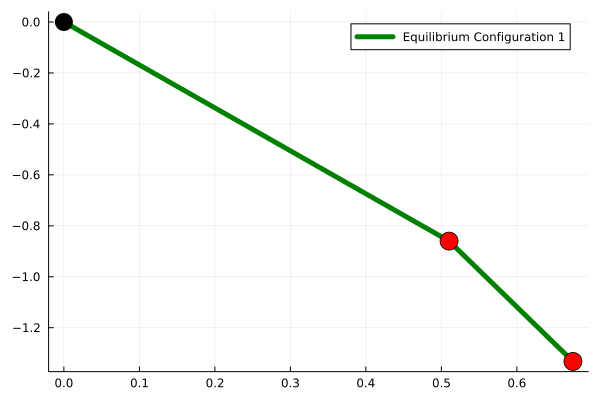
\includegraphics[width=0.45\columnwidth]{graphics/Chap09/EquilibriumWithSprings.png}
    \end{center}
\bigskip
The following code implements a Newton-Raphson routine to find $G(q_1^\ast, q_2^\ast) = [0; 0]$.
\bigskip

\begin{lstlisting}[language=Julia,style=mystyle]
using LinearAlgebra
include("dyn_mod_2LinkManipulatorWithSprings.jl") 
x0 = [pi/2, pi/4] 
Model = dyn_mod_2LinkManipulatorWithSprings(x0, 0*x0)
G = Model.G
JacG = Model.JacG
k = 0
aTol = 1e-5
s = 0.1
xk = x0
while (k<1e5)&&(norm(G)>aTol)
    k = k+1
    Delta_x = -JacG\G
    xk = xk + s*Delta_x
    Model = dyn_mod_2LinkManipulatorWithSprings(xk, 0*xk)
    G = Model.G
    JacG = Model.JacG
end
Model = dyn_mod_2LinkManipulatorWithSprings(xk, 0*xk)
G = Model.G
JacG = Model.JacG

display(G)
[xk x0] 
\end{lstlisting}
\textbf{Output} 
\begin{verbatim}
2-element Vector{Float64}:
 -2.959527982682175e-6
  9.381671145725079e-6
  
2×2 Matrix{Float64}:
 -1.03536   1.5708
 -0.201158  0.785398
\end{verbatim}



  \bigskip
\begin{tcolorbox}[colback=mylightblue, title = {\bf Linearization About an Equilibrium Point}, breakable]

Let $x_e \in \real^n$ be an \textbf{equilibrium point} of the differential equation $\dot{x} = f(x)$ and suppose that $f$ is differentiable at $x_e$. Then from \eqref{eq:AffineMatrixApprox05}, the linearization of $f$ about $x_e$ is
$$ f(x) = f(x_e) + \left. \frac{\partial f(x)}{\partial x}\right|_{x = x_e} (x-x_e) = \frac{\partial f(x_e)}{\partial x}\cdot (x-x_e),$$
where $f(x_e) = 0_{n \times 1}$ follows from $x_e$ being an equilibrium point.\\

  \begin{definition} 
   \label{def:linearizedODE}
   For a nonlinear vector ODE $\dot{x} = f(x)$, the \textbf{linearization about an equilibrium point} $x_e$ is the linear vector ODE
\begin{equation}
 \label{eq:linearizedODE}
\delta  \dot{x} =   \frac{\partial f(x_e)}{\partial x}\cdot \delta x,  
\end{equation}
where $\delta x:= x - x_e$.
\end{definition}
 \vspace*{.1cm}
\textbf{Notes:} 
\begin{itemize}
    \item If $\delta x(t)$ is a solution to the linearized model \eqref{eq:linearizedODE}, then $x_e + \delta x(t)$ is an \textbf{approximate solution} to the original nonlinear model.
    \item When $x_e=0_{n \times 1}$, it common to write the linearized model as $\dot{x} = A x$, for $A:=\frac{\partial f(x_e)}{\partial x}$, thereby dropping the $\delta$.
    \item Even when $x_e \neq 0_{n \times 1}$, it is still rather uncommon to use $\delta x$ as the name of the state variables in the linear model. Some engineers abuse notation and reuse the variable $x$, others opt for a new variable name, such as $z$ or $\chi$. 
\end{itemize}
\end{tcolorbox}

 \bigskip

 \begin{example} 
\label{ex:linearizeAboutEquilibriumPoints}
Linearize the following nonlinear models about the given equilibrium points. 
 \begin{enumerate}
\renewcommand{\labelenumi}{(\alph{enumi})}
\setlength{\itemsep}{.2cm}
    \item $\frac{dv(t)}{dt} =   \frac{\kappa}{m} v^2(t) - g$ with $v_e = -\sqrt{ \frac{m\,g}{\kappa} }$ (parachutist with nonlinear drag, from Example~\ref{ex:ChuteODE04}).
    
    \item $\left[ \begin{array}{c} \dot{x}_1 \\ \dot{x}_2 \end{array} \right]= \left[\begin{array}{c} x_2 \\  -\frac{g}{L}  \cdot \sin(x_1)\end{array} \right]$ with $x_e = \left[ \begin{array}{c} 0\\ 0 \end{array} \right]$ and $x_e = \left[ \begin{array}{c} \pi \\ 0 \end{array} \right]$ (pendulum model from Examples~\ref{ex:PendulumModel} and \ref{ex:PendulumModelTake2}).

\end{enumerate} 
\end{example}
\textbf{Solutions:}
 \begin{enumerate}
\renewcommand{\labelenumi}{(\alph{enumi})}
\setlength{\itemsep}{.8cm}
    \item $\dot{v} =   \frac{\kappa}{m} v^2 - g$ \quad \Ans \quad $ \delta \dot{v} = -\left(2 \sqrt{\frac{\kappa \, g}{m}}\, \right) \cdot \delta v$ , where $\delta v = v-v_e$.\\

We identify $f(v)=\frac{\kappa}{m} v^2 - g$ and compute $\frac{df(v)}{dv} = \frac{d}{dv} (\frac{\kappa}{m} v^2 - g) = 2 \frac{\kappa}{m} v$. Evaluating the ``Jacobian'' at $v_e = -\sqrt{ \frac{m\,g}{\kappa} }$ gives $\frac{df(v_e)}{dv} = -2 \sqrt{\frac{\kappa \, g}{m}}$. Hence, the linearized model is
    $$ \delta \dot{v} = -\left(2 \sqrt{\frac{\kappa \, g}{m}} \, \right) \cdot \delta v,~~\delta v = v-v_e.$$
    
    \textbf{Note:} The scalar coefficient in front of $\delta v$ is negative. Later, we'll see that this imparts a ``self-stabilizing action'' to the model, meaning that if the velocity is initially greater than the equilibrium velocity, then it will decrease toward the equilibrium velocity, and conversely, if the velocity is initially lower than the equilibrium velocity, then it will increase toward the equilibrium velocity. If this were not the case, the parachutist would have to continually adjust the surface area of the parachute to regulate their speed, considerably augmenting the difficulty of the jump!
    
    \item $\left[ \begin{array}{c} \dot{x}_1 \\ \dot{x}_2 \end{array} \right]= \left[\begin{array}{c} x_2 \\  -\frac{g}{L}  \cdot \sin(x_1)\end{array} \right]$ \quad  \Ans \quad $\left[ \begin{array}{c} \dot{x}_1 \\ \dot{x}_2 \end{array} \right] =  \left[\begin{array}{cc} 0 & 1 \\  -\frac{g}{L} & 0\end{array} \right] \left[ \begin{array}{c}{x}_1 \\ {x}_2 \end{array} \right]  ~~\text{and}~~
\left[ \begin{array}{c} \delta \dot{x}_1 \\ \delta \dot{x}_2 \end{array} \right] =  \left[\begin{array}{cc} 0 & 1 \\  \frac{g}{L} & 0\end{array} \right] \left[ \begin{array}{c}\delta {x}_1 \\ \delta {x}_2 \end{array} \right]$.  \\ \\

We identify $f(x) = f(x_1, x_2) = \left[\begin{array}{c} x_2 \\  -\frac{g}{L}  \cdot \sin(x_1)\end{array} \right]$ and compute $\frac{\partial f(x_1, x_2)}{\partial x} =  \left[\begin{array}{cc} 0 & 1 \\  -\frac{g}{L}  \cdot \cos(x_1) & 0\end{array} \right]$. Evaluating the Jacobian at the two equilibria gives
$$\frac{\partial f(0, 0)}{\partial x} =  \left[\begin{array}{cc} 0 & 1 \\  -\frac{g}{L} & 0\end{array} \right] \quad ~~\text{and}~~\quad
\frac{\partial f(\pi, 0)}{\partial x}= \left[\begin{array}{cc} 0 & 1 \\  \frac{g}{L} & 0\end{array} \right]. $$
Hence, the two linear models are 
$$ \left[ \begin{array}{c} \dot{x}_1 \\ \dot{x}_2 \end{array} \right] =  \left[\begin{array}{cc} 0 & 1 \\  -\frac{g}{L} & 0\end{array} \right] \left[ \begin{array}{c}{x}_1 \\ {x}_2 \end{array} \right] \quad ~~\text{and}~~\quad
\left[ \begin{array}{c} \delta \dot{x}_1 \\ \delta \dot{x}_2 \end{array} \right] =  \left[\begin{array}{cc} 0 & 1 \\  \frac{g}{L} & 0\end{array} \right] \left[ \begin{array}{c}\delta {x}_1 \\ \delta {x}_2 \end{array} \right], $$
where in the first model, because the equilibrium is at the origin, we kept $x$ as the state variable, and in the second model, we are using $\left[ \begin{array}{c}\delta {x}_1 \\ \delta {x}_2 \end{array} \right]:= \left[ \begin{array}{c} {x}_1 - \pi\\{x}_2 \end{array} \right].$ There are no hard and fast rules governing these choices. You have a lot of freedom to do what you prefer.\\

\textcolor{red}{\bf Note:} The two linear models differ by a minus sign in the (2,1) position of the ``$A$-matrix''. Later, we'll see that the ``$A$-matrix'' of the first model has purely imaginary eigenvalues $\lambda = \pm \im \sqrt{\frac{g}{L}}$, indicating oscillatory behavior, while the second model has two real eigenvalues $\lambda = \pm \sqrt{\frac{g}{L}}$, with the positive eigenvalue indicating ``instability''. This comports with what we know about an inverted (aka, upward pointing) pendulum: if we perturb it ever so slightly, it will fall over and not return to the upright position, while if we perturb a normal pendulum, it will oscillate. Segways, BallBots, bipedal robots, and humans each contain an (unstable) inverted pendulum that must be balanced! If this were not the case, babies would have a ``self-righting'' mechanism built in at birth. 
\end{enumerate} 
\Qed

  \bigskip

  \begin{propColor}{Linearization of the Robot Equations}{LinearizedRobotEquations}
We initially encountered the robot equations expressed as a set of nonlinear second-order differential equations,
$$ D(q) \cdot \ddot{q} + C(q, \dot{q}) \cdot \dot{q} + G(q) = 0_{n \times 1}, $$
where we are assuming here that there are no external forces acting on the robot. In Example~\ref{ex:equilibriumPoints}, we determined that their equilibrium points correspond to $G(q_e) = 0_{n \times 1}$ and $\dot{q}_e=0_{n \times 1}$. Their linearization about an equilibrium can be expressed in both second-order and first-order forms, namely,
\begin{equation}
    \label{eq:RobotEqnLinearizedSecondOrder}
    D(q_e) \cdot \delta \ddot{q} + \frac{\partial G(q_e)}{\partial q} \cdot \delta q = 0_{n \times 1},
\end{equation}
where $\delta q = q-q_e$, and
\begin{equation}
    \label{eq:RobotEqnLinearizedSecondOrderV02}
  \left[ \begin{array}{c} \delta \dot{x}_1 \\ \delta  \dot{x}_2 \end{array} \right] = \left[ \begin{array}{cc} 0_n & I_n \\ A_{21} & 0_n \end{array} \right] \left[ \begin{array}{c} \delta {x}_1 \\ \delta {x}_2 \end{array} \right], 
\end{equation}
where $A_{21}= -D(q_e) \backslash \frac{\partial G(q_e)}{\partial q}$ because we know not to invert large matrices, $I_n$ is the $n \times n$ identity matrix, $\delta x_1 = q- q_e$, and $\delta x_2 = \dot{q} - 0_{n \times 1}$.\\

\textbf{Note:} At first, it is surprising that the term $C(q, \dot{q}) \cdot \dot{q}$ does not show up in the linearization. The reason is that it consists of quadratic terms of the form $c_{ij}(q) \cdot \dot{q}_i \cdot \dot{q}_j$, which when linearized about $\dot{q}_e=0_{n \times 1}$, $1 \le i \le n$, all vanish. By taking advantage of this property, the linearization of the robot equations is trivial to compute: you only have to compute one Jacobian, $\frac{\partial G(q_e)}{\partial q}$, and evaluate the mass inertia matrix at $q_e$. 

% \textbf{Note:} The proof is immediate once you learn enough about Lagrangian Dynamics to know that each term of the vector $ C(q, \dot{q}) \cdot \dot{q} $ is a linear combination of terms of the form $\alpha_{ij}(q) \dot{q}_i \cdot \dot{q}_j$, and hence, they drop out when evaluating their Jacobian at an equilibrium point, $(q_e, 0_{n \times n})$.
  \end{propColor}

    \bigskip

\begin{example}
\label{ex:linearizedModel3LinkManipulator}
    
    In Chapter~\ref{sec:3LinkLagrangeEquations}, we derived Lagrange's equations for a 3-link manipulator. Using Julia, compute its linearized model about the downward equilibrium, $q_e^{d}=\left[ \begin{array}{c} -\frac{\pi}{2}\\ 0 \\0\end{array} \right]$ and the upward equilibrium $q_e^{u}=\left[ \begin{array}{c} \frac{\pi}{2}\\ 0 \\0\end{array} \right]$. \\

    Use the following function to define physical values to the parameters.
\begin{lstlisting}[language=Julia,style=mystyle]
function modelParameters()
    g = 9.81 # m/s^2
    L1 = 1 # m
    L2 = 0.7
    L3 = 0.5
    m1 = 15 # kg
    m2 = 10
    m3 = 5    
    return g, L1, L2, L3, m1, m2, m3
end
\end{lstlisting}

    \end{example}
    \textbf{Solutions:} ~~ \newline
    \Ans \quad \textbf{Downward Equilibrium}
 $$\left[ \begin{array}{c} \dot{x}_1\\ \dot{x}_2 \\ \dot{x}_3 \\ \dot{x}_4 \end{array} \right]
 = \left[ \begin{array}{rrrrrr}
0.0000 & 0.0000 & 0.0000 & 1.0000 & 0.0000 & 0.0000 \\
0.0000 & 0.0000 & 0.0000 & 0.0000 & 1.0000 & 0.0000 \\
0.0000 & 0.0000 & 0.0000 & 0.0000 & 0.0000 & 1.0000 \\
\BLUE -9.8100 & \BLUE 9.8100 & \BLUE 0.0000 & 0.0000 & 0.0000 & 0.0000 \\
\BLUE 9.8100 & \BLUE -37.8386 & \BLUE 7.0071 & 0.0000 & 0.0000 & 0.0000 \\
\BLUE 0.0000 & \BLUE 28.0286 & \BLUE -36.4371 & 0.0000 & 0.0000 & 0.0000 \\
\end{array} \right] \cdot \left[ \begin{array}{c} x_1\\ x_2 \\ x_3 \\x_4 \\ x_4 \\ x_6\end{array} \right]
$$
    \bigskip
\Ans \quad \textbf{Upward Equilibrium}
 $$\left[ \begin{array}{c} \dot{x}_1\\ \dot{x}_2 \\ \dot{x}_3 \\ \dot{x}_4 \end{array} \right]
 = \left[
\begin{array}{rrrrrr}
0.0000 & 0.0000 & 0.0000 & 1.0000 & 0.0000 & 0.0000 \\
0.0000 & 0.0000 & 0.0000 & 0.0000 & 1.0000 & 0.0000 \\
0.0000 & 0.0000 & 0.0000 & 0.0000 & 0.0000 & 1.0000 \\
\RED 9.8100 & \RED -9.8100 & \RED 0.0000 & 0.0000 & 0.0000 & 0.0000 \\
\RED -9.8100 & \RED 37.8386 & \RED -7.0071 & 0.0000 & 0.0000 & 0.0000 \\
\RED 0.0000 & \RED -28.0286 & \RED 36.4371 & 0.0000 & 0.0000 & 0.0000 \\
\end{array}
\right] \cdot \left[ \begin{array}{c} x_1\\ x_2 \\ x_3 \\x_4 \\ x_4 \\ x_6\end{array} \right]
$$

\textcolor{red}{\bf Note:} The $A_{21}$ block for the upward equilibrium is the negative of the $A_{21}$ block for the downward equilibrium. This generalizes to three-links the observation we made for the single-link pendulum. In Example~\ref{ex:eigenvaluesLinearizedModel3LinkManipulator}, we explore what this means for the eigenvalues of the respective linearized models. 


  \vspace*{.4cm}  
  \textcolor{blue}{\bf The \texttt{function dyn\_mod\_3LinkManipulator(q, dq)}} (see file \texttt{dyn\_mod\_3LinkManipulator.jl
}),  \textcolor{blue}{\bf returns (D=D, C=C, G=G, B=B, JacG=JacG)}, where ${\rm JacG } = \frac{\partial G}{\partial q}.$ We will use $D$ and $JacG$.\\

 We only show the code for the downward equilibrium.   

\begin{lstlisting}[language=Julia,style=mystyle]
# Linear Model for the 3-link Manipulator
#
# bring the model into the workspace for later use
include("dyn_mod_3LinkManipulator.jl") 

#Build a function to define the parameters of the model

function modelParameters()
    g = 9.81 # m/s^2
    L1 = 1 # m
    L2 = 0.7
    L3 = 0.5
    m1 = 15 # kg
    m2 = 10
    m3 = 5    
    return g, L1, L2, L3, m1, m2, m3
end

# Set equilibirum Point
if true
    qe = [-pi/2, 0, 0]
else
    qe = [pi/2, 0, 0]
end

F = dyn_mod_3LinkManipulator(qe, 0*qe)
D = F.D; display(D)
JacG = F.JacG; display(JacG)

# build the linearized model about the give equilibrium point
A21 = -D\JacG; A21 = cleanUp(A21); display(A21)
n, ~ = size(A21)
A = [zeros(n,n) I(n); A21 zeros(n,n)]

\end{lstlisting}
\textbf{Output} 
\begin{verbatim}
3×3 Matrix{Float64}:
 68.1  25.1  5.5
 25.1  12.1  3.0
  5.5   3.0  1.25
  
3×3 Matrix{Float64}:
 421.83   127.53   24.525
 127.53   127.53   24.525
  24.525   24.525  24.525
  
3×3 Matrix{Float64}:
 -9.81    9.81      0.0
  9.81  -37.8386    7.00714
  0.0    28.0286  -36.4371
  
6×6 Matrix{Float64}:
  0.0     0.0       0.0      1.0  0.0  0.0
  0.0     0.0       0.0      0.0  1.0  0.0
  0.0     0.0       0.0      0.0  0.0  1.0
 -9.81    9.81      0.0      0.0  0.0  0.0
  9.81  -37.8386    7.00714  0.0  0.0  0.0
  0.0    28.0286  -36.4371   0.0  0.0  0.0
\end{verbatim}
    \Qed

    \bigskip

\begin{example} 
\label{ex:eigenvaluesLinearizedModel3LinkManipulator}
Use Julia to compute the eigenvalues of both linearized models in Example~\ref{ex:linearizedModel3LinkManipulator}. 
   
\end{example} 
\textbf{Solutions:} \quad \Ans \quad$ \left[ \begin{array}{c} \lambda_1\\ \lambda_2 \\ \lambda_3 \\\lambda_4 \\ \lambda_5 \\ \lambda_6\end{array} \right]^d = \left[
\begin{array}{r}
-7.2389 \im \\
7.2389 \im \\
-2.4528 \im \\
2.4528 \im \\
-5.0664 \im \\
5.0664 \im \\
\end{array}
\right]$ \quad and \quad \Ans \quad $\left[ \begin{array}{c} \lambda_1\\ \lambda_2 \\ \lambda_3 \\\lambda_4 \\ \lambda_5 \\ \lambda_6\end{array} \right]^u = \left[
\begin{array}{r}
-7.2389 \\
-5.0664 \\
-2.4528 \\
2.4528 \\
5.0664 \\
7.2389 \\
\end{array}
\right]$.

\bigskip

\textcolor{red}{\bf Note:} For the downward equilibrium, the eigenvalues are distinct and purely imaginary, which we will later show implies sustained periodic behavior. For the upward equilibrium, on the other hand, the eigenvalues are real and occur in positive-negative pairs, $\pm \lambda$. We'll see later that the positive real eigenvalues imply ``instability'', meaning solutions have norms that tend to infinity. Yikes! \\

\textbf{(Optional Read:)} Is there a logical explanation for why the eigenvalues change so drastically from one model to the other? Yes. There are two explanations. The first explanation is based on our physical experience with inverted pendula, as we discussed in Example\ref{ex:equilibriumPoints}-(b); one the system is disturbed, it topples over. The second and more mathematical explanation is that for the robot equations, we have
\[ A = \begin{bmatrix} 0_n & I_n \\ A_{21} & 0_n \end{bmatrix}. \]
When \( A_{21} \) is an invertible \( n \times n \) matrix, 
\href{https://math.stackexchange.com/questions/262563/eigenvalues-of-block-matrices-with-zero-diagonal-blocks}{one can show that}
\[ \det(\lambda I_{2n}- A ) = \det\begin{bmatrix} \lambda I_n & -I_n \\ -A_{21} & \lambda I_n \end{bmatrix} = \det(\lambda^2 I_n - A_{21}). \]
Therefore, the eigenvalues of \( A \) are the plus and minus square roots of the eigenvalues of \( A_{21} \). That's pretty cool! The sign change on the entries of $A_{21}$ for upward and downward equilibria changes purely imaginary eigenvalues into purely real eigenvalues. The reason behind the sign change of the entries of $A_{21}$ is more technical. It arises because in the upward equilibrium, the potential energy is a maximum, while at the lower equilibrium, it is a minimum. Indeed, because $G(q) = \nabla PE(q)$, $\frac{\partial G(q)}{\partial q}$ is the Hessian of the potential energy. The Hessian is a positive definite matrix at a local minimum and a negative definite matrix at a local maximum. Linear Algebra is very powerful!\\


\vspace*{.4cm}

\textbf{Code for the Downward Equilibrium}
\begin{lstlisting}[language=Julia,style=mystyle]
E=eigen(A)
evals = cleanUp(E.values); display(evals)
\end{lstlisting}
\textbf{Output} 
\begin{verbatim}
6-element Vector{ComplexF64}:
 0.0 - 7.23885032225449im
 0.0 + 7.23885032225449im
 0.0 - 2.452784229773624im
 0.0 + 2.452784229773624im
 0.0 - 5.066419822703628im
 0.0 + 5.066419822703628im
\end{verbatim}

\textbf{CleanUp Function that handles complex numbers}

\begin{lstlisting}[language=Julia,style=mystyle]
function cleanUp(A, tol=1e-10)
    B = copy(A)
    for i in eachindex(B)
        if isa(B[i], Complex)
            # Clean up the real part
            real_part = abs(real(B[i])) < tol ? 0.0 : real(B[i])
            # Clean up the imaginary part
            imag_part = abs(imag(B[i])) < tol ? 0.0 : imag(B[i])
            # Reconstruct the complex number
            B[i] = real_part + imag_part * im
        else
            # Original cleanup for non-complex numbers
            if abs(B[i]) < tol
                B[i] = 0.0
            end
        end
    end
    return B
end
\end{lstlisting}
\textbf{Output} 
\begin{verbatim}
cleanUp (generic function with 2 methods)
\end{verbatim}



\subsection{The Matrix Exponential}
\label{sec:MatrixExponential}

We recall that for $a \in \real$, the Maclaurin/Taylor Expansions for $e^{at}$ and $e^{a(t-t_0)}$ are
\begin{equation}
    \begin{aligned}
        e^{at}&= \sum_{k=0}^\infty a^k \cdot \frac{t^k}{k!} = 1 + a \cdot t + a^2 \cdot \frac{t^2}{2!} + \cdots + a^k \cdot \frac{t^k}{k!} + \cdots ~~\text{and}\\[1em]
        e^{a(t-t_0)}&= \sum_{k=0}^\infty a^k \cdot \frac{(t-t_0)^k}{k!} = 1 +a \cdot (t-t_0) + a^2 \cdot \frac{(t-t_0)^2}{2!} + \cdots + a^k \cdot \frac{(t-t_0)^k}{k!} + \cdots, \\[1em]
    \end{aligned}
\end{equation}
respectively\footnote{The definition should be written as $e^{at}=1 + \lim_{N \to \infty} \sum_{k=1}^N a^k \cdot \frac{t^k}{k!}$ so that the need for a limit is clear, and so that we do not have to use $0^0=1$. Normally, these ``niceties'' are assumed to be understood by the reader.}. In the following, we initially take $t_0=0$, so that the Maclaurin and Taylor expansions are the same.

\bigskip

\begin{tcolorbox}[colback=mylightblue, title = {\bf Matrix Exponential and Exponential Function}, breakable]
In the following, $I_n$ denotes the $n \times n$ identity matrix.
\begin{definition}
For $A$ an $n \times n$ real matrix,
\begin{equation}
    \label{eq:matrixExponential}
  e^{A}:=  \sum_{k=0}^\infty A^k \cdot \frac{1}{k!} = I_n + A  + A^2 \cdot \frac{1}{2!} + \cdots + A^k \cdot \frac{1}{k!} + \cdots \\[1em]
\end{equation}
is called the \textbf{matrix exponential}. It is also denoted as $\exp(A)$. \\

\textbf{Note:} If $A=0_{n}$, the $n \times n$ zero matrix, then $\exp(0_n):=I_n$. \textcolor{red}{\bf Warning: This shows that the matrix exponential is not the exponential of each term of the matrix.}  In other symbols, $\left[e^{A}\right]_{ij} \neq \exp(a_{ij})$. If it were, then $\exp(0_n)$ would equal an $n \times n$ matrix filled with ones, instead of being an identity matrix.\\

\end{definition}

\begin{definition}
For $A$ an $n \times n$ real matrix and $t\in \real$,
\begin{equation}
    \label{eq:matrixExponentialFunction}
  e^{A t}:=  \sum_{k=0}^\infty A^k \cdot \frac{t^k}{k!} = I_n + A \cdot t + A^2 \cdot \frac{t^2}{2!} + \cdots + A^k \cdot \frac{t^k}{k!} + \cdots \\[1em]
\end{equation}
is called the \textbf{matrix exponential function}. It is also denoted as $\exp(At)$. \\

\end{definition}
\bigskip
\textbf{Notes:} \,
\begin{itemize}
    \item The matrix exponential function is simply the matrix exponential evaluated at the matrix $A\cdot t = t \cdot A$, which depends upon time. 
    \item One is often lazy and refers to $e^{A t}$ as the matrix exponential instead of the matrix exponential ``function'' because context usually makes the true meaning very clear.
    \item A more formal definition of the matrix exponential is $e^{A}:= I_n +  \displaystyle \lim_{N \to \infty}\sum_{k=1}^N A^k \cdot \frac{1}{k!}$, making the need to evaluate a limit clear. Using techniques from Michigan's Math 451, the existence of the limit can be established for ALL $n \times n$ matrices with entries in $\real$ or $\cp$.
\end{itemize}

\end{tcolorbox}

\bigskip
\begin{example} 
\label{ex:matrixExponentialFunctionHandComputation}
Using the series definition, compute $e^{At}$ for 
 \begin{enumerate}
\renewcommand{\labelenumi}{(\alph{enumi})}
\setlength{\itemsep}{.2cm}
     \item $A_1 = \left[ \begin{array}{cc} a_{11} & 0\\0 & a_{22}\end{array}\right]$,
     \item $A_2=\begin{bmatrix}\lambda_{1} & 0 & 0\\
0 & \ddots & 0\\
0 & 0 & \lambda_{n}
\end{bmatrix} $, and
     \item $A_3 = \left[ \begin{array}{rr} 0 & 1\\-1 & 0\end{array}\right]$.
\end{enumerate}    
\end{example}
\textbf{Solutions:} In each case, we need to find a pattern that makes evaluating the infinite sum feasible. The first two problems are remarkably easy.

 \begin{enumerate}
\renewcommand{\labelenumi}{(\alph{enumi})}
\setlength{\itemsep}{.8cm}
     \item $A_1 = \left[ \begin{array}{cc} a_{11} & 0\\0 & a_{22}\end{array}\right] {\BLUE \implies} e^{A_1  t} = \left[ \begin{array}{cc} e^{a_{11}t} & 0\\0 & e^{a_{22}t} \end{array}\right] $.\\

     Before applying the definition, we note that raising a diagonal matrix to a power gives a diagonal matrix with entries raised to the same power, that is, 
     $$ \left[ \begin{array}{cc} a_{11} & 0\\0 & a_{22}\end{array}\right]^{\scalebox{1.0}{$k$}} = \underbrace{ \left[ \begin{array}{cc} a_{11} & 0\\0 & a_{22}\end{array}\right] \times \cdots \times \left[ \begin{array}{cc} a_{11} & 0\\0 & a_{22}\end{array}\right]  }_{k-\text{times}} = \left[ \begin{array}{cc} \left(a_{11}\right)^k & 0\\0 & \left(a_{22}\right)^k\end{array}\right], $$
     as is easily checked for $k=2$ and $k=3$. The general case follows by induction (which would be good practice). Using this result, we have,
 \begin{align*}
 e^{A_1  t} &= I_2 + \left[\begin{array}{cc} a_{11} & 0 \\ 0 & a_{22} \end{array} \right]  \cdot t +  \left[ \begin{array}{cc} \left(a_{11}\right)^2 & 0\\0 & \left(a_{22}\right)^2\end{array}\right] \cdot \frac{t^2}{2!} + \cdots + \left[ \begin{array}{cc} \left(a_{11}\right)^k & 0\\0 & \left(a_{22}\right)^k\end{array}\right]  \cdot \frac{t^k}{k!} + \cdots \\[1em]
 & = \left[\begin{array}{cc} 1 & 0 \\ 0 & 1 \end{array} \right] + \left[\begin{array}{cc} a_{11} t & 0 \\ 0 & a_{22}t \end{array} \right]   +  \left[ \begin{array}{cc} \left(a_{11}\right)^2 \frac{t^2}{2!}& 0\\0 & \left(a_{22}\right)^2 \frac{t^2}{2!}\end{array}\right]  + \cdots + \left[ \begin{array}{cc} \left(a_{11}\right)^k \frac{t^k}{k!}& 0\\0 & \left(a_{22}\right)^k \frac{t^k}{k!}\end{array}\right]   + \cdots \\[1em]
 & = \left[ \begin{array}{cc} e^{a_{11}t} & 0\\0 & e^{a_{22}t} \end{array}\right].     
 \end{align*}
         
    
     \item $A_2=\begin{bmatrix}\lambda_{1} & 0 & 0\\
0 & \ddots & 0\\
0 & 0 & \lambda_{n}
\end{bmatrix} {\BLUE \implies} e^{A_2 t} = \begin{bmatrix}e^{\lambda_{1} t} & 0 & 0\\
0 & \ddots & 0\\
0 & 0 & e^{\lambda_{n} t}
\end{bmatrix} $ \\

The calculations follow exactly the same steps as part (a) and are left to the learner.

     \item $A_3 = \left[ \begin{array}{rr} 0 & 1\\-1 & 0\end{array}\right] {\BLUE \implies} e^{A_3t} =  \left[ \begin{array}{rr}\cos(t) & \sin(t) \\ - \sin(t) & \cos(t) \end{array}\right]$. \\
     
     Let's pause for just a moment and appreciate that a matrix exponential of a real-valued matrix can oscillate, while scalar exponentials of real variables are monotonic.  Later, in Definition~\ref{def:complexExponentials} and Prop.~\ref{thm:PropertiesComplexExponentials}, we'll discover that this remarkable feature comes from Euler's formula, $e^{\im \theta} = \cos(\theta) + \im \sin(\theta)$, or, if we replace $\theta$ with $\omega t$, \fbox{$ e^{\im \omega t} = \cos(\omega t) + \im \sin(\omega t).$}\\

     \textbf{To reduce clutter, we replace $A_3$ with $A$ in the following.} \\

     The pattern occurring in the powers of $A$ is more ``subtle'' this time. The first few powers are straightforward: by brute force multiplication, we obtain,      
$$A^0 = I_2, \quad A=\begin{bmatrix}0 & 1 \\ -1 & 0  \end{bmatrix}, \quad
A^2=\begin{bmatrix}-1 & 0 \\ 0 & -1  \end{bmatrix},  \quad A^3=\begin{bmatrix}0 & -1 \\ 1 & 0  \end{bmatrix}, \quad
A^4=\begin{bmatrix}1 & 0 \\ 0 & 1  \end{bmatrix}=I_2,$$
where we notice that $ A^4 $ brings us back to where we started, the identity matrix. That is the pattern we are seeking! 

We note immediately that
$$ A^{4k} = \underbrace{A^4 \times \cdots \times A^4}_{\text{k times}} = I_2 \times \cdots \times I_2 =I_2.$$
Next, 
$$ A^{4k+0}=I_2, \quad A^{4k+1}=A=\begin{bmatrix}0 & 1 \\ -1 & 0  \end{bmatrix}, \quad A^{4k+2}=A^2=\begin{bmatrix}-1 & 0 \\ 0 & -1  \end{bmatrix}, \quad A^{4k+3}=A^3=\begin{bmatrix}0 & -1 \\ 1 & 0  \end{bmatrix},$$ \\
which is kind of amazing the first time you see it.\\

To compute $e^{At}$, we need to substitute the above results into our power series for the matrix exponential,
$$e^{At}=I_2+At+A^2 \frac{t^2}{2!}+A^3 \frac{t^3}{3!}+A^4\frac{t^4}{4!}+ +A^5\frac{t^5}{5!}\cdots.$$
By doing so, we obtain
\begin{align*}
\left[e^{At} \right]_{11} &= 1 + 0 - \frac{t^2}{2}+0+\frac{t^4}{4!} + \cdots = \cos(t) \\[1em]
\left[e^{At} \right]_{12}  &= 0+t+0 - \frac{t^3}{3!}+0+\frac{t^5}{5!} + \cdots = \sin(t) \\[1em]
\left[e^{At} \right]_{21} &= 0 - t + 0 +\frac{t^3}{3!}+0-\frac{t^5}{5!} + \cdots = -\sin(t) \\[1em]
\left[e^{At} \right]_{22}  &= 1 + 0 - \frac{t^2}{2}+0+\frac{t^4}{4!} + \cdots = \cos(t),    
\end{align*}
after recognizing the Maclaurin/Taylor expansions for cosine and sine. Therefore, 
$$e^{At}=\begin{bmatrix} ~~\cos(t) & \sin(t) \\ - \sin(t) & \cos(t) \end{bmatrix}.$$
\end{enumerate} 
% \begin{eqnarray*}
% e^{At} & = & I+\begin{bmatrix}\lambda_{1} & 0 & 0\\
% 0 & \ddots & 0\\
% 0 & 0 & \lambda_{n}
% \end{bmatrix}t+\frac{1}{2!}\begin{bmatrix}\lambda_{1} & 0 & 0\\
% 0 & \ddots & 0\\
% 0 & 0 & \lambda_{n}
% \end{bmatrix}^{2}t^{2}+\frac{1}{3!}\begin{bmatrix}\lambda_{1} & 0 & 0\\
% 0 & \ddots & 0\\
% 0 & 0 & \lambda_{n}
% \end{bmatrix}^{3}t^{3}+\cdots\\
%  & = & \begin{bmatrix}e^{\lambda_{1}t} & 0 & 0\\
% 0 & \ddots & 0\\
% 0 & 0 & e^{\lambda_{n}t}
% \end{bmatrix}
% \end{eqnarray*}


\Qed

\bigskip
\subsection{Software Tools}

 As you should probably expect by now, there are software tools to help you with computing both $\bm{e^A}$ (the matrix exponential) and $\bm{e^{At}}$ (the matrix exponential function). We illustrate these next.

 \bigskip

\begin{lstlisting}[language=Julia,style=mystyle]
using LinearAlgebra
# Mass spring damper system
m = 5 # kg
k = 2 # N/m
b = 3 # Ns/m (Newton seconds per meter)
A = [0 1; -k/m -b/m]
expA = exp(A)
\end{lstlisting}
\textbf{Output} 
\begin{verbatim}
2×2 Matrix{Float64}:
  0.839867  0.703132
 -0.281253  0.417988
\end{verbatim}

\bigskip
Below is a comparison between the builtin function and a highly truncated implementation of the power series. You can see that the power series converges rapidly. This rapid convergence means that a finite number of terms well approximates the matrix exponential. We will differentiate with respect to time the matrix exponential \textbf{function} in the next subsection, using an argument based on the matrix exponential being well approximated by a finite number of terms. Its formal proof relies on analytically proving the absolute convergence of the Maclaurin/Taylor expansions for the matrix exponential, a step we will not take in this course. Bonjour, Math 451 Advanced Calculus!\\

\begin{lstlisting}[language=Julia,style=mystyle]
# Compare to the builtin exp function
N=9
expA2 = I(2)
AkOverKfactorial = I(2)
for k = 1:N
    AkOverKfactorial = A*AkOverKfactorial/k
    expA2 = expA2 + AkOverKfactorial    
end
[expA expA2]
\end{lstlisting}
\textbf{Output} 
\begin{verbatim}
2×4 Matrix{Float64}:
  0.839867  0.703132   0.839867  0.703132
 -0.281253  0.417988  -0.281253  0.417988
\end{verbatim}


\bigskip \textbf{Note:} In Matlab, you would use \texttt{expA = expm(A)}, where the ``m'' appended to ``exp'' tells Matlab to compute the matrix exponential. Continuing with Matlab, the command, \texttt{expA = exp(A)} would compute the exponential of each term of the matrix, which is very much not the matrix exponential. Because Julia uses \textbf{broadcasting} to apply a scalar function to a vector- or matrix-valued object, it does not need the \texttt{expm( )} command. 

\begin{lstlisting}[language=Julia,style=mystyle]
# Comparison of exp(A) and exp.(A)
[exp(A) exp.(A)] # Not the same
\end{lstlisting}
\textbf{Output} 
\begin{verbatim}
2×4 Matrix{Float64}:
  0.839867  0.703132  1.0      2.71828
 -0.281253  0.417988  0.67032  0.548812
\end{verbatim}

\bigskip
For large square matrices, the matrix exponential can be computed numerically. \textbf{The symbolic computation of the matrix exponential function, on the other hand, is limited to ``smallish matrices with simple structure''.} \textcolor{blue}{\bf In practice, this tends not to be an issue, because of eigenvalues and eigenvectors, as we'll highlight in the next section.} \\

We continue with ``modest'' results on symbolic calculations applied to Example~\ref{ex:matrixExponentialFunctionHandComputation}.

\begin{lstlisting}[language=Julia,style=mystyle]
using SymPy
# 
@vars a11 a22 t
A1 = [a11 0; 0 a22]
A1t = A1*t  # Define a 2x2 square matrix
expA1t =exp(A1t)  # Compute the matrix exponential function
\end{lstlisting}
\textbf{Output} 
$$
\left[
\begin{array}{cc}
e^{a11 \cdot t} & 0.0 \\
0.0 & e^{a22 \cdot t} \\
\end{array}
\right]
$$

\begin{lstlisting}[language=Julia,style=mystyle]
using SymPy
# 
@vars lam1 lam2  lam3 lam4 t
A2 = Diagonal([lam1, lam2,  lam3, lam4])
A2t = A2*t  # Define a 2x2 square matrix
expA2t =exp(A2t)  # Compute the matrix exponential function
\end{lstlisting}
\textbf{Output} 
$$\left[
\begin{array}{cccc}
e^{lam1 \cdot t} & 0.0 & 0.0 & 0.0 \\
0.0 & e^{lam2 \cdot t} & 0.0 & 0.0 \\
0.0 & 0.0 & e^{lam3 \cdot t} & 0.0 \\
0.0 & 0.0 & 0.0 & e^{lam4 \cdot t} \\
\end{array}
\right]$$

\begin{lstlisting}[language=Julia,style=mystyle]
using SymPy
# 
@vars t
A3 = [0 1; -1 0]
A3t = A3*t  # Define a 2x2 square matrix
expA3t =exp(A3t)  # Compute the matrix exponential function
\end{lstlisting}
\textbf{Output} 
$$\left[
\begin{array}{cc}
\frac{e^{\im \cdot t}}{2.0} + \frac{e^{\left(  - \im \right) \cdot t}}{2.0} & \frac{\left(  - \im \right) \cdot e^{\im \cdot t}}{2.0} + \frac{\im \cdot e^{\left(  - \im \right) \cdot t}}{2.0} \\[1em]
\frac{\im \cdot e^{\im \cdot t}}{2.0} - \frac{\im \cdot e^{\left(  - \im\right) \cdot t}}{2.0} & \frac{e^{\im \cdot t}}{2.0} + \frac{e^{\left(  -\im \right) \cdot t}}{2.0} \\
\end{array}
\right]$$
You must know Euler's Formula from Chapter~\ref{sec:IntroEulerFormula} to understand the answer! Moreover, for $\sin(t)$, you must recognize that 
$$ \frac{\left(  - \im \right) \cdot e^{\im \cdot t}}{2.0} + \frac{\im \cdot e^{\left(  - \im \right) \cdot t}}{2.0}  = \frac{e^{\im \cdot t}- e^{-\im \cdot t}}{2 \im} $$
because $\frac{1}{\im} = \frac{1}{\im}\cdot \frac{\im}{\im} = -\im$. Currently, applying \texttt{SymPy.simplify} to the answer does not help. 


\bigskip

\subsection{Solutions to Linear ODEs}

\begin{propColor}{Derivative of the Matrix Exponential Function}{DerivativeMatrixExponentialFunction}
For all $t \in \real$ and all $n \times n$ (constant) matrices,
\begin{equation}
    \label{derivMatrixExonentialFunction}
    \frac{d}{dt} e^{A \cdot t} = A \cdot e^{A \cdot t}= e^{A \cdot t} \cdot A.
\end{equation}

% \bigskip
% \textbf{Note:} 

\end{propColor}



\bigskip

\begin{example}  (Optional Read:)  Give a non-rigorous but mostly persuasive argument that \eqref{derivMatrixExonentialFunction} holds.
    
\end{example}
\textbf{Solution:} The obstruction to being rigorous is that we do not have enough math to understand when the derivative of an infinite sum is the infinite sum of the derivatives. Hence, we approximate the matrix exponential by a finite sum,
$$e^{At} \approx e_N^{A \cdot t}:= I_n + \sum_{k=1}^N A^{k} \cdot \frac{t^{k}}{k!} = I_n + A \cdot t + A^2 \cdot \frac{t^2}{2!} + A^3 \cdot \frac{t^3}{3!}+  \cdots +  A^{N-1} \cdot \frac{t^{N-1}}{(N-1)!} +   A^{N} \cdot \frac{t^{N}}{N!},$$
where $N$ sets the number of terms in the approximation. We can now use the fact that the derivative of a finite sum is the finite sum of the derivatives.

% Because the derivative of a finite sum is the sum of the derivatives, we have 
% \begin{align*}
%     \frac{d}{dt} e_{N}^{A \cdot t} &= \frac{d}{dt}\left(  I_n + A \cdot t + A^2 \cdot \frac{t^2}{2!} + A^3 \cdot \frac{t^3}{3!}+  \cdots +  A^{N-1} \cdot \frac{t^{N-1}}{(N-1)!} +   A^{N} \cdot \frac{t^{N}}{N!} \right) \\
%     & = 0_n + A + A^2 \cdot 2\frac{t^1}{2!} +  A^3 \cdot 3\frac{t^2}{3!} + \cdots + A^{N-1} \cdot (N-1)\frac{t^{N-2}}{(N-1)!} + A^{N} \cdot N\frac{t^{N-1}}{N!} \\
%       &=  A + A^2 \cdot \frac{t^1}{1!} +   A^3 \cdot \frac{t^2}{2!}+ \cdots + A^{N-1} \cdot \frac{t^{N-2}}{(N-2)!} + A^{N} \cdot \frac{t^{N-1}}{(N-1)!} \\
%       &= A\left( I_n +  A \cdot t + A^2 \cdot \frac{t^2}{2!} + \cdots + A^{N-2} \cdot \frac{t^{N-2}}{(N-2)!} + A^{N-1} \cdot \frac{t^{N-1}}{(N-1)!}  \right) \\
%       & = A \cdot e_{(N-1)}^{A \cdot t}.
% \end{align*}
Computing derivatives term by term gives
\begin{align*}
    \frac{d}{dt} I_n & = 0_n~~\text{and} \\[1em]
    \frac{d}{dt} \left(A^{k} \cdot \frac{t^{k}}{k!} \right)& = A^{k} \cdot k \cdot  \frac{t^{k-1}}{k!} \\
    & =  A^{k} \cdot \frac{t^{k-1}}{(k-1)!} \\
    &= A \left( A^{k-1} \cdot \frac{t^{k-1}}{(k-1)!}\right) =   \left( A^{k-1} \cdot \frac{t^{k-1}}{(k-1)!}\right) A,
\end{align*}
where we note that $A$ can be factored to either side. \\

Using the above result, 
\begin{align*}
    \frac{d}{dt} \underbrace{\left( I_n + \sum_{k=1}^N A^{k} \cdot \frac{t^{k}}{k!} \right)}_{\approx e^{At}} & = 0_n +  \sum_{k=1}^N A \left( A^{k-1} \cdot \frac{t^{k-1}}{(k-1)!} \right) \\[1em]
    & = A \sum_{k=1}^N  \left( A^{k-1} \cdot \frac{t^{k-1}}{(k-1)!} \right)\\[1em]
    &= A \cdot \underbrace{\left( I_n + \sum_{k=1}^{N-1}  \frac{t^{k}}{k!} \right)}_{\approx e^{At}}.
\end{align*}
Once again, we note that when $A$ was factored out, it could have gone to either side. This completes our ``mostly'' persuasive argument.\\

\textbf{Note:} This is the same ``proof'' offered in EECS 560 Linear Systems Theory because it does not assume real analysis. 
\Qed

\vspace{.2cm}

\begin{propColor}{Explicit Solution to a Linear System of ODEs}{SolutionsLinearODEs}

The unique solution to $\dot{x} = A \cdot x, ~x(t_0) = x_0$ is
\begin{equation}
\label{eq:MatrixExponentialSolutionODE}
\varphi(t, t_0,x_0):= e^{A(t-t_0)} \cdot x_0.
\end{equation} 

\bigskip
\textbf{Note:} It is perfectly fine to denote the solution by $\varphi(t)= e^{A(t-t_0)} \cdot x_0$, dropping the explicit dependence on the initial time, $t_0$, and the initial state, $x_0$, or to use $\varphi(t, x_0)= e^{A t} \cdot x_0$, when $t_0=0$. You are in control of your own notation when communicating results to your colleagues.
\end{propColor}

\bigskip
\textbf{Proof:} All the conditions of Def.~\ref{def:ODEsolution} are met; indeed:
\begin{itemize}
    \item  Prop.~\ref{thm:DerivativeMatrixExponentialFunction} states that the matrix exponential is differentiable; it follows that it must be continuous (meaning that each of the entries of the matrix exponential function is continuous in $t$). 
    \item $\varphi(t_0, t_0, x_0):= e^{A(t_0-t_0)} \cdot x_0 = I_n \cdot x_0 = x_0 $~~(\text{satisfies the initial condition}).
    \item $\frac{\partial }{ \partial t} \varphi(t, t_0, x_0):= \left(\frac{\partial }{ \partial t} e^{A(t-t_0)} \right) \cdot x_0 = \left(A \cdot e^{A(t-t_0)} \right) \cdot x_0 = A \cdot e^{A(t-t_0)}\cdot x_0 =$ 
    ${ A \cdot \varphi(t, t_0, x_0)}$~~(\text{satisfies the differential equation}). 
\end{itemize}

We already noted in Def.~\ref{def:ODEsolution} why the solution is unique. Indeed, by Prop.~\ref{thm:MatrixVectorCalculusFormulas}-(a), $\frac{\partial}{\partial x} \left( Ax \right) = A$ is independent of $x$. Hence, Prop.~\ref{thm:ExistenceUniquenessSolutionsODEs}-(b) implies that for all $x_0\in \real^n$, $t_0\in \real$, there exists a solution on $[t_0, \infty)$ and the solution is unique.  
\Qed

\bigskip

\begin{center}
\setlength{\fboxrule}{2pt}  % Setting the thickness of the border line
   \fbox{ \parbox{0.9\linewidth}{
   \vspace{.15cm} 

\textcolor{blue}{\bf One rarely uses \eqref{eq:MatrixExponentialSolutionODE} to compute the solution to a real engineering problem. Instead, one uses solvers, such as ``DifferentialEquations.jl''. \textcolor{red}{\bf Equation \eqref{eq:MatrixExponentialSolutionODE} is used to deduce GENERAL PROPERTIES of SOLUTIONS to linear ODES, while a solver is used to COMPUTE SOLUTIONS for GIVEN INITIAL CONDITIONS.}}
\vspace{.15cm} 
}
} 
\end{center}


\bigskip

\begin{example} 
\label{ex:MassSpringDamperCompareSolutionMethods}
Compute the solution to the mass-spring-damper system in Example~\ref{ex:MassSpringDamperNoGravity}, using two methods:
\begin{itemize}
    \item A numerical solver, such as \texttt{DifferentialEquations.jl}
    \item Prop.~\ref{thm:SolutionsLinearODEs}.
\end{itemize}
Take the parameters as mass m = 5 Kg, spring constant k = 2 N/m (Newtons per meter), and damping coefficient b = 3 Ns/m (Newton seconds per meter). 
\end{example}
\textbf{Solution:}


\begin{lstlisting}[language=Julia,style=mystyle]
# Import useful packages
using DifferentialEquations
using Plots 
using LaTeXStrings
using LinearAlgebra # for the backslash command
gr()

# Mass spring damper system
m = 5 # kg
k = 2 # N/m
b = 3 # Ns/m (Newton seconds per meter)
A = [0 1; -k/m -b/m]

# Define the ODE
function MassSpringDamper(du, x, A, t) 
    du .= A*x
end


# Set the initial condition as a vector
x0=[1; 0.0]

# Set the time interval
T = (0.0, 20) 

# Setup the ODE problem
params = A 
problem = ODEProblem(MassSpringDamper, x0, T, params)

# solve the ODE problem using the Runge Kutta Tsitouras 5/4 Integrator
sol = solve(problem, Tsit5())

# plot the continuous solution
p1 = plot(sol, lw=3, guidefont=20, xlabel=L"t", ylabel=L"(x, v)", 
    label=["x" "v"], legend=:topright)


# Discrete time vector
t=0:dt:T[2]

# use a for loop to compute the matrix exponential for A*t[k] and
# then multiply by the initial condition to get the solution at t[k]
N = length(t)
x = zeros(2, N)
for k = 1:length(t)
    x[:,k] = exp(A*t[k])*x0
end

# Overlay the discrete-time solution with the continuous-time solution
scatter!(t, x[1,:], label = false, color=:blue)
scatter!(t, x[2,:], label = false, color=:red)
\end{lstlisting}
\textbf{Output} 
The solid lines are the solutions from the numerical solver, while the dots are the points computed by evaluating the matrix exponential function at $t_k = k \cdot 0.4$ seconds, for $0 \le k \le 50$. They are indistinguishable.
\begin{center}
    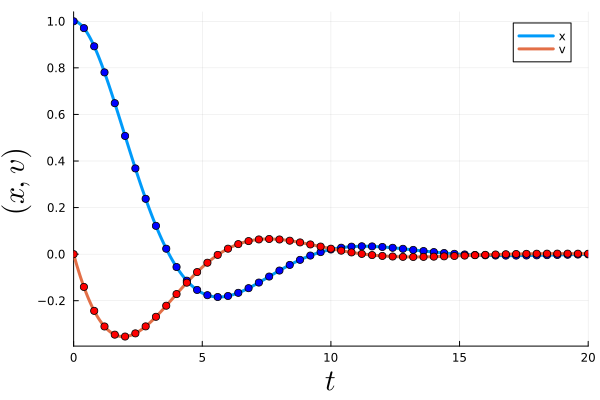
\includegraphics[width=0.6\columnwidth]{graphics/Chap09/MassSpringDamperComparisonSimulationChap09.png}
\end{center}
\Qed

\bigskip

\begin{propColor}{(Optional Read:) Useful Properties of the Matrix Exponential}{keyPropertiesMatrixExponential}

Here we highlight the similarities and differences between the matrix exponential function and the scalar exponential function. For $A$ an $n \times n $ matrix,
 \begin{enumerate}
\renewcommand{\labelenumi}{(\alph{enumi})}
\setlength{\itemsep}{.2cm}
    \item $\det\left(e^{A}\right) = e^{\trace(A)}$, where $\trace(A)$ is the sum of its diagonal elements, and
    \item $e^{A (s+t)} = e^{A s}  \cdot e^{A t} $ for all real numbers $s$ and $t$.
\end{enumerate}
The first property says that, like the scalar exponential function, the matrix exponential is always invertible. The second property is similar to $e^{as} \cdot e^{at} = e^{a(s + t)}$, though it has a more profound interpretation in terms of solutions of linear ODEs. In particular, if we define $\varphi(t, t_0, x_0):=e^{A(t-t_0)} \cdot x_0$, then
\begin{align*}
\varphi(s+t, t_0, x_0) &:=e^{A (s+t-t_0)} \cdot x_0 \\
& =  e^{A s} \cdot e^{A (t-t_0)} \cdot x_0 \\
&= e^{A s} \cdot \varphi(t,  t_0, x_0). 
\end{align*}
In other words, multiplying on the left by the matrix exponential $e^{A (t-t_0)}$ transitions the solution of $\dot{x} = Ax, x(t_0)=x_0$ from the value of the solution at the initial time, $t_0$, to the value of the solution at time $t$, and multiplying on the left again by the matrix exponential $e^{A s}$ transitions the solution from time $t$ to time to $s+t$. \\

Property (b) implies the following two additional properties,
\bigskip
 \begin{enumerate}
\renewcommand{\labelenumi}{(\alph{enumi})}
\setlength{\itemsep}{.2cm}
\setcounter{enumi}{2}
 \item $\left(e^{A t}\right)^{-1} = e^{-A t}  $ for all real numbers $t$, and
    \item $\left(e^{A t_d}\right)^k = e^{A \cdot k \cdot t_d}  $ for all real numbers $t_d$ and integers $k$.
    \end{enumerate} 

\bigskip

\textbf{A key difference between the scalar exponential function and the matrix exponential function involves $\bm{e^{(A + B)t} }$, for $\bm{B}$ an $\bm{n \times n} $ matrix.}

\begin{enumerate}
\renewcommand{\labelenumi}{(\alph{enumi})}
\setlength{\itemsep}{.2cm}
\setcounter{enumi}{4}
    \item $e^{(A + B)t} = e^{A t} \cdot e^{B t} \iff  A\cdot B - B \cdot A = 0_{n}$, which in words says the matrix exponential of a sum of matrices equals the product of the matrix exponentials if, and only if, $A$ and $B$ commute. Since most matrices do not commute, it is generally false that the matrix exponential of a sum is equal to the product of the matrix exponentials. Of course, if the matrices are $1 \times 1$, meaning they are scalars, then they also commute. \end{enumerate} 

\end{propColor}

\bigskip

\textbf{Note:} Even in graduate engineering courses, we typically do not cover the proofs of the above properties. Their main steps are related to proof by induction and binomial expansion.  If you do want the proofs, we suggest \href{https://en.wikipedia.org/wiki/Matrix_exponential}{Matrix exponential} by Wikipedia. Another source is \href{http://scipp.ucsc.edu/~haber/webpage/MatrixExpLog.pdf}{Notes on the Matrix Exponential and Logarithm} by the Santa Cruz Institute for Particle Physics. Finally, some interesting comments are available on the Mathematical Stack Exchange, \href{https://math.stackexchange.com/questions/1854759/proof-of-matrix-exponential-property-e-textbf-a-textbf-b-e-textbf-ae-t#:~:text=Proof%20of%20matrix%20exponential%20property%20eA%2BB%3DeA,if%20AB%3DBA&text=I%20know%20how%20to%20prove,)%3D0%20for%20all%20t.}{Proof that exp(A+B) = exp(A)*exp(B) iff AB = BA}.

\bigskip

\subsection{Eigenvalues and Eigenvectors to the Rescue}

\begin{center}
\setlength{\fboxrule}{2pt}  % Setting the thickness of the border line
   \fbox{ \parbox{0.9\linewidth}{
   \vspace{.15cm} 
   
   \textcolor{blue}{\bf Punchline for this Section:} We've given several hints that eigenvalues are important. In this Section, we confirm it! From the eigenvalues of $A$, we can determine whether all solutions of $\dot{x} = A x$ remain bounded and converge to zero as $t$ goes to infinity, there are sustained oscillations, or some solutions tend to infinity. The reason behind this phenomenal fact? \textbf{If $\lambda$ is an eigenvalue of $A$ with eigenvector $v$, then $e^{\lambda t}$ is an eigenvalue of $e^{At}$ with corresponding eigenvector $v$.} When $\lambda$ is real, it is easy to understand whether $e^{\lambda t}$ converges to zero or explodes. Thanks to Euler's Formula, we can also handle the case of complex eigenvalues.
}
} 
\end{center}

\subsubsection{Review of Complex Numbers}

If you wish a more extensive review of complex numbers, see ROB 101 \textit{Computational Linear Algebra}, Appendix A.1. Here, we recall just a few facts. For $\alpha, \beta \in \real$, and $\im^2 = -1$,
$$z := \alpha + \im \beta$$
is a \textbf{complex number}. Its \textbf{complex conjugate} is 
$$z^\ast:= \alpha - \im \beta,$$
where the sign is flipped on the imaginary part.
A \textbf{complex vector} is simply a vector with entries that are complex numbers. Hence, it can be written as
$$v:= v_R + \im v_I,$$
where $v_R, v_I \in \real^n$; $v_R$ is called the \textbf{real part} of the vector and $v_I$ is called the \textbf{imaginary part} of the vector. It is important to understand that the imaginary part DOES NOT include $\im$, the imaginary unit number, and thus $v_I$ is a real vector. The complex conjugate of the vector is 
$$v^\ast:= v_R - \im v_I,$$
where the sign is flipped on the imaginary part. Finally, the \textbf{magnitude} of the complex number $z^\ast:= \alpha + \im \beta$ is defined to be
$$|z|:=\sqrt{\alpha^2 + \beta^2} = \sqrt{z \cdot z^\ast}.$$
The \textbf{(Euclidean) norm of a complex vector} is
$$||v||:= \sqrt{\left(v^\ast\right)^\top \cdot v} = \sqrt{\sum_{i=1}^n |v_i|^2},$$
where $v_i$ are the components of $v$. Just as with norms of real vectors, $$||\alpha v|| = |\alpha| \cdot ||v||,$$
for all $\alpha \in \cp$ and $v \in \cp^n$.
\\

\subsubsection{Eigenvalues and Eigenvectors of Matrices}
We next recall from ROB 101 \textit{Computational Linear Algebra}, Chapter 10.3 and Appendix A.2, the definition of eigenvalues and eigenvectors for $n \times n$ matrices.

\bigskip
\begin{tcolorbox}[colback=mylightblue, title = {\bf Definition of Eigenvalues and Eigenvectors}, breakable]
%
\begin{definition}
\label{def:EignStuff}
  Let $A$ be an $n\times n$ matrix with real or complex coefficients. A scalar $\lambda \in  \cp$ is an \textbf{eigenvalue} of $A$, if there exists a non-zero vector $v \in \cp^{n}$ such that $Av=\lambda v$. Any such vector $v$ is called an \textbf{eigenvector} associated with $\lambda$. \\
\end{definition}
 
\textbf{Notes:} 
\begin{itemize}
    \item Eigenvectors are not unique. If $v$ is an eigenvector, then so is $\alpha \cdot v$ for any nonzero constant $\alpha$. 
    \item Most Linear Algebra packages normalize the eigenvector to have norm one.
    \item If $A$ is a real matrix and $\lambda \in \real$, then we take $v \in \real^n$.
    \item If $A$ is a real matrix and $\lambda \in \cp$ satisfies $Av = \lambda v$, then $\lambda^\ast$, the complex conjugate of $\lambda$, is also an eigenvalue of $A$ with corresponding eigenvector, $v^\ast$. In particular, $A v^\ast = \lambda^\ast v^\ast$. We say the eigenvalues and eigenvectors occur in \textbf{complex conjugate pairs}.
\end{itemize} 
\end{tcolorbox}


\bigskip
\begin{center}
\setlength{\fboxrule}{2pt}  % Setting the thickness of the border line
   \fbox{ \parbox{0.9\linewidth}{
   \vspace{.15cm} 
   
   \textcolor{blue}{\bf This next example helps to understand why eigenvalues tell us so much about solutions to linear systems of ODEs, 
   $$\bm{\dot{x}=A\cdot x,~~x(t_0=0)=x_0},$$ 
   in particular, when the solutions converge to the origin, oscillate, or blow up.} 
}
} 
\end{center}

\bigskip
\begin{example} \textcolor{red}{\bf (Must Read:)} The $2 \times 2$ matrix  $A = \left[
\begin{array}{rr}
a & \omega \\
-\omega & a
\end{array}
\right]$ has eigenvalues $\lambda_1= a + \im \omega$ and $\lambda_2= a - \im \omega$ . Use \texttt{SymPy} to compute $e^{At}$. \textcolor{red}{\bf On the basis of $\bm{e^{At}}$, interpret the qualitative behavior of the solutions to the linear ODE $\bm{\dot{x} = Ax}$ when the real parts of the eigenvalues} \textbf{are negative, zero, and positive.}
\end{example}
\textbf{Solution:}

\begin{lstlisting}[language=Julia,style=mystyle]
using SymPy

@vars a w t
A = [a w; -w a]*t  # Define a 2x2 square matrix
expA = A.exp()  # Another way to compute the matrix exponential
\end{lstlisting}
\textbf{Output} 

$$
\left[
\begin{array}{cc}
\frac{e^{a \cdot t - \im \cdot t \cdot w}}{2.0} + \frac{e^{a \cdot t + \im \cdot t \cdot w}}{2.0} & \frac{ \im \cdot e^{a \cdot t - \im \cdot t \cdot w}}{2.0} - \frac{ \im \cdot e^{a \cdot t + \im \cdot t \cdot w}}{2.0} \\[1em]
\frac{\left(  - \im \right) \cdot e^{a \cdot t - \im \cdot t \cdot w}}{2.0} + \frac{ \im \cdot e^{a \cdot t + \im \cdot t \cdot w}}{2.0} & \frac{e^{a \cdot t - \im \cdot t \cdot w}}{2.0} + \frac{e^{a \cdot t + \im \cdot t \cdot w}}{2.0} \\
\end{array}
\right] = \left[
\begin{array}{rr}
e^{at} \cos(\omega t) & e^{at} \sin(\omega t) \\
-e^{at} \sin(\omega t) & e^{at} \cos\omega t) 
\end{array}
\right].
$$

\bigskip

The simplification on the right was done by hand, based on  
\begin{align*}
    \frac{e^{a \cdot t - \im \cdot t \cdot \omega}}{2.0} +  \frac{e^{a \cdot t + \im \cdot t \cdot \omega}}{2.0}&=  e^{at} \left( \frac{e^{ - \im \cdot t \cdot \omega} + e^{\im \cdot t \cdot \omega}}{2} \right)\\
     &= e^{at} \left( \frac{ \cos(t \cdot \omega)  -  \im \sin(t \cdot \omega) + \cos(t \cdot \omega) + \im \sin(t \cdot \omega)}{2} \right) \\
    &= e^{at} \, \cos(\omega\, t) \\
    \\
        \frac{\im \, e^{a \cdot t - \im \cdot t \cdot \omega}}{2.0} -  \frac{\im e^{a \cdot t + \im \cdot t \cdot \omega}}{2.0}&=  e^{at} \left( \frac{ \im e^{ - \im \cdot t \cdot \omega} - \im  e^{\im \cdot t \cdot \omega}}{2} \right)\\
        &= e^{at} \left( \frac{ \im \cos(t \cdot \omega)  +  \sin(t \cdot \omega)- \im \cos(t \cdot \omega) + \sin(t \cdot \omega)}{2} \right) \\
    &= e^{at} \, \sin(\omega\, t) .  
\end{align*}
Thanks to eigenvalues and eigenvectors, \textbf{complex exponentials}, aka exponentials of the form, $e^{\left( a + \im \omega \right) t}$, play a fundamental role in understanding the solutions of linear systems of ODEs.\\

For the present problem, we note that for all $x_0 \neq 0_{2 \times 1}$, the solution of $\dot x = Ax, \, x(t_0=0)=x_0$,
   $$\varphi(t, t_0,x_0):=\left[
\begin{array}{rr}
e^{a t} \cos(\omega t) & e^{a t} \sin(\omega t) \\
-e^{a t} \sin(\omega t) & e^{a t} \cos(\omega t) 
\end{array}
\right] \cdot \left[ \begin{array}{c}
x_{01} \\
x_{02}
\end{array}
\right], $$
\begin{itemize}
    \item converges to zero if $a < 0$ (decaying exponentially) when eigenvalues have a negative real part;
    \item oscillates forever if $a = 0$ (no exponential term) when eigenvalues are purely imaginary; and
    \item blows up if $a >0$ (exploding exponentially) when eigenvalues have a positive real part. 
\end{itemize}

\Qed


\bigskip


\begin{example} 
Use Julia to compute the eigenvalues and eigenvectors of the $3 \times 3$ matrix 
$$A:=\left[
\begin{array}{rrr}
1.3916 & -0.4173 & -1.0494 \\
-0.4823 & -0.4498 & -0.2974 \\
1.1709 & -0.2278 & 1.9801 \\
\end{array}
\right].$$
Moreover, verify the following properties:
\begin{enumerate}
\renewcommand{\labelenumi}{(\alph{enumi})}
\setlength{\itemsep}{.2cm}
    \item The eigenvalues and eigenvectors occur in complex conjugate pairs.
    \item $Av = \lambda v$.
    \item The eigenvectors are linearly independent and hence form a basis for $\cp^3$.
    \item If $v=v_R + \im v_I$ is a complex eigenvector, then $v$  and its complex conjugate $v^\ast$ can be replaced by $v_R$ and $v_I$, the real and imaginary parts of $v$, to build a basis for $\real^3$.
\end{enumerate}
\end{example}
\textbf{Solutions:}

\begin{enumerate}
\renewcommand{\labelenumi}{(\alph{enumi})}
\setlength{\itemsep}{.6cm}
    \item The eigenvalues and eigenvectors occur in complex conjugate pairs.\\
   
\begin{lstlisting}[language=Julia,style=mystyle]
using LinearAlgebra

A = [1.39164   -0.417337  -1.04938
     -0.482258  -0.449806  -0.297397
      1.1709    -0.2278     1.98006]

E = eigen(A)
\end{lstlisting}
\textbf{Output} 
\begin{verbatim}
Eigen{ComplexF64, ComplexF64, Matrix{ComplexF64}, Vector{ComplexF64}}
values:
3-element Vector{ComplexF64}:
 -0.5492714681705643 + 0.0im
  1.7355827340852823 - 1.0454627840167563im
  1.7355827340852823 + 1.0454627840167563im
vectors:
3×3 Matrix{ComplexF64}:
    0.206377+0.0im    0.17411+0.639401im     0.17411-0.639401im
    0.978444+0.0im   0.105157-0.0907931im   0.105157+0.0907931im
 -0.00741578+0.0im  -0.735901-0.0im        -0.735901+0.0im
\end{verbatim}

Hence, the eigenvalues are 
$$ \lambda_1 = -0.5493+0.0000\im , \quad \lambda_2 = 1.7356-1.0455\im, \quad \lambda_3 = 
1.7356+1.0455\im,$$
and the corresponding eigenvectors are 
$$v_1 = \left[
\begin{array}{r}
0.2064+0.0000\im  \\
0.9784+0.0000\im  \\
-0.0074+0.0000\im  \\
\end{array}
\right], \quad v_2 = 
\left[
\begin{array}{r}
0.1741+0.6394\im  \\
0.1052-0.0908\im  \\
-0.7359+0.0000\im  \\
\end{array}
\right], \quad v_3 = 
\left[
\begin{array}{r}
0.1741-0.6394\im  \\
0.1052+0.0908\im  \\
-0.7359+0.0000\im  \\
\end{array}
\right].
$$
$\lambda_1$ is real, with real eigenvector $v_1$, while $\lambda_2$ and $\lambda_3$ are complex, with complex eigenvectors, $v_2$ and $v_3$. Moreover, $\lambda_3 = \lambda_2^\ast$ and $v_3 = v_2^\ast$.  

 \item $Av = \lambda v$. \\
   

\begin{lstlisting}[language=Julia,style=mystyle]
# verify A*v = lambda*v
for k = 1:3
    v=E.vectors[:,k]
    lam = E.values[k]
    display([A*v lam*v])
end
\end{lstlisting}
The columns of $\left[ Av~~~~\lambda v\right]$ are identical.\\

\textbf{Output} 
\begin{verbatim}
3×2 Matrix{ComplexF64}:
  -0.113357+0.0im   -0.113357+0.0im
  -0.537432+0.0im   -0.537432+0.0im
 0.00407327+0.0im  0.00407327-0.0im
 
3×2 Matrix{ComplexF64}:
  0.970653+0.927707im   0.970653+0.927707im
 0.0875883-0.267517im  0.0875883-0.267517im
  -1.27722+0.769357im   -1.27722+0.769357im
  
3×2 Matrix{ComplexF64}:
  0.970653-0.927707im   0.970653-0.927707im
 0.0875883+0.267517im  0.0875883+0.267517im
  -1.27722-0.769357im   -1.27722-0.769357im
\end{verbatim}

 \item The eigenvectors are linearly independent and hence form a basis for $\cp^3$.
\begin{lstlisting}[language=Julia,style=mystyle]
# Check for a basis
V=E.vectors

# Note V' computes the complex conjugate transpose of the complex matrix V
# V'*V is theoretically guaranteed to have a real determinant, though
# numerically, it may have a small imaginary part

# Check linear independence of the columns of V
det(V'*V)
\end{lstlisting}
\textbf{Output} 
\begin{verbatim}
0.897060699129927 + 1.6064687371449844e-18im
\end{verbatim}

We see that the determinant equals $0.8971 + \im 1.6065 \times 10^{-18}$, that is, the imaginary part is the numerical equivalent of zero. Because the determinant is nonzero, the columns of $V$ are linearly independent. \\

\textbf{(Optional Read:) Note:} $V'\cdot V : = \left(V^\ast\right)^\top \cdot V$ is a \href{https://en.wikipedia.org/wiki/Hermitian_matrix}{\textbf{Hermitian Matrix}}, that is a square matrix that is equal to the transpose of its (complex) conjugate matrix. The diagonal elements of a Hermitian matrix are all real numbers, and the element of the (i, j) position is equal to the (complex) conjugate of the element in the (j, i) position. In our case,
$$ V'\cdot V : = \left(V^\ast\right)^\top \cdot V = \left[
\begin{array}{ccc}
1.0000+0.0000\im & 0.1443+0.0431\im & 0.1443-0.0431\im \\
0.1443-0.0431\im & 1.0000+0.0000\im & 0.1658-0.2036\im \\
0.1443+0.0431\im & 0.1658+0.2036\im & 1.0000+0.0000\im \\
\end{array}
\right],$$
satisfies all of these properties.

\item If $v=v_R + \im v_I$ is a complex eigenvector, then $v$  and its complex conjugate $v^\ast$ can be replaced by $v_R$ and $v_I$, the real and imaginary parts of $v$, to build a basis for $\real^3$.\\

The vectors $V_{\rm new}:=[v_1, {\rm real}(v_2), {\rm imag}(v_2) ]$ are linearly independent because the determinant of $V_{\rm new}^\top \cdot V_{\rm new}$ equals 0.224 and hence is nonzero.

\begin{lstlisting}[language=Julia,style=mystyle]
# real(E.vectors[:,1]) removes the zero imaginary part and makes it 
# a Float64 instead a ComplexF64

# real(E.vectors[:,2]) computes the real part of v2
# imag(E.vectors[:,2]) computes the imaginary part of v2

# Stack candidate basis vectors as columns of V_new
V_new = [real(E.vectors[:,1]) real(E.vectors[:,2]) imag(E.vectors[:,2])]

display(V_new)

# Check linear independence
det(V_new'*V_new)
\end{lstlisting}
\textbf{Output} 
\begin{verbatim}
3×3 Matrix{Float64}:
  0.206377     0.17411    0.639401
  0.978444     0.105157  -0.0907931
 -0.00741578  -0.735901  -0.0
 
0.22426517478248179
\end{verbatim}
 
\end{enumerate}
\Qed



\subsubsection{Eigenvalues and Eigenvectors of the Matrix Exponential}

\textcolor{blue}{\bf Remarkably, eigenvectors of $A$ are also eigenvectors of $e^{At}$, for all $t\in \real$, while the eigenvalues are transformed under the exponential map in a simple manner.} 

\bigskip

\begin{propColor}{Eigenvalues and Eigenvectors of the Matrix Exponential}{EigenStuffMatrixExponential}
Suppose that $A$ is an $n \times n$ real matrix and that $Av = \lambda v$, with $v\neq 0_{n \times 1}$. Then, the following are true,
 \begin{enumerate}
\renewcommand{\labelenumi}{(\alph{enumi})}
\setlength{\itemsep}{.2cm}
    \item $A^k \cdot v = \lambda^k v$ for all integers $k \ge 1$, 
    \item $e^{A} \cdot v = e^{\lambda} v$, and
    \item $e^{A t} \cdot v = e^{\lambda t} v$ for all $t \in \real$.
\end{enumerate} 
Hence, if $v\neq 0_{n \times 1}$ is an eigenvector of $A$ with corresponding eigenvalue $\lambda$, then $v$ is an eigenvector of the matrix exponential function, $e^{At}$, with corresponding eigenvalue $e^{\lambda t}$. The surprising part is that only the eigenvalue is a function of time, and it (aka, $e^{\lambda t}$) is either a standard (real) exponential function of time or a complex exponential function of time. The eigenvectors of $e^{At}$ are constant and identical to the eigenvectors of $A$.
\end{propColor}

\bigskip
\textbf{Proof:} (a) is proved by induction. We know the base case holds because we assumed that $Av = \lambda v$. Hence, assume $A^k \cdot v = \lambda^k v$ holds for some $k\ge 1$; we need to show it holds for $k+1$. 
\begin{align*}
    A^{k+1} \cdot v &= A \cdot \left(A^k \cdot v \right)  ~~(\text{algebra}) \\
   &=  A \cdot \left(\lambda^k \cdot v \right) ~~(\text{by the induction hypothesis}) \\
    &= \lambda^k \cdot \left( A\cdot v \right) ~~(\text{algebra, swapped the order of } A \text{ and } ~\lambda^k) \\
    &= \lambda^k \cdot \left( \lambda v \right) ~~(\text{because }Av = \lambda v) \\
    & =  \lambda^{k+1} v   ~~(\text{algebra}).
\end{align*}

To prove (b), we use (a) with the power series for the matrix exponential, namely,
\begin{align*}
   e^A \cdot v &= \left(I_n + \sum_{k=1}^\infty \frac{t^k}{k!} A^k \right) \cdot v  ~~(\text{definition of}~e^A) \\
    &=   v +  \sum_{k=1}^\infty \frac{t^k}{k!} A^k \cdot v ~~(\text{multiply through by}~v)\\
    &= v + \sum_{k=1}^\infty \frac{t^k}{k!} \lambda^k \cdot v ~~(\text{from part (a)})\\
     &= \left( 1+ \sum_{k=1}^\infty \frac{t^k}{k!} \lambda^k \right) \cdot v ~~(\text{factor out }~v)\\[1em]
     &= e^{\lambda t} v~~ (\text{apply the definition of }~e^{\lambda t}).
\end{align*}

Part (c) is obtained from (b) by substituting $At$ in place of $A$. 
\Qed.

\bigskip

\begin{example}
\label{ex:FirstPeekComplexExponentials}
    Use the eigenvectors of $A=\left[
\begin{array}{rr}
-2.7690 & -4.1472 \\
0.6061 & 1.2690 
\end{array}
\right]$ as initial conditions for $\dot{x} = Ax.$ Observe the ``qualitative properties'' of the corresponding solutions. 
\end{example}
\textbf{Solution:}
Let's find the eigenvalues and eigenvectors of $A$.
\begin{lstlisting}[language=Julia,style=mystyle]
using LinearAlgebra

A = [-2.76899   -4.14723; 0.606141   1.26899]

E = eigen(A)
\end{lstlisting}
\textbf{Output} 
\begin{verbatim}
Eigen{Float64, Float64, Matrix{Float64}, Vector{Float64}}
values:
2-element Vector{Float64}:
 -2.0000057922545804
  0.50000579225458
vectors:
2×2 Matrix{Float64}:
 -0.98324    0.785355
  0.182314  -0.619045
\end{verbatim}

Hence, the eigenvalues 
$$ \lambda_1 = -2, \quad \lambda_2 = 0.5$$
are both real and distinct, and the corresponding eigenvectors are 
$$v_1 = \left[
\begin{array}{r}
-0.983240  \\
 0.182314
\end{array}
\right], \quad v_2 = 
\left[
\begin{array}{r}
0.785355\\
-0.619045
\end{array}
\right]
$$
are real and linearly independent. \\

We note that $\lambda_1 < 0$ while $\lambda_2>0$. We next compute and plot solutions to $\dot{x}=Ax$, with $x_0 = v_1$ and $x_0 = v_2$. In fact, we are going to plot the norm of each solution, $||e^{At} x_0||$. We show only the code for the first eigenvector as the initial condition.

\begin{lstlisting}[language=Julia,style=mystyle]
# Compute and plot ||x(t) = exp(At)*x0|| for x0 an eigenvector.
using Plots
using LinearAlgebra
using LaTeXStrings

function normSolution(t; A=A, x0=E.vectors[:,1])
    eAt = exp(A*t)
    xt = eAt * x0
    y = norm(xt)
    return y
end

# time values where we compute the solution
t = 0:.1:8

y = normSolution.(t)

p1 = plot(t,y, guidefont = 20, legend = false, xlabel=L"t", ylabel=L"||e^{At}\cdot x_0 ||", lw=3, 
    color=:blue)
\end{lstlisting}
\textbf{Output} 
\begin{center}
    \begin{minipage}{0.45\columnwidth}
        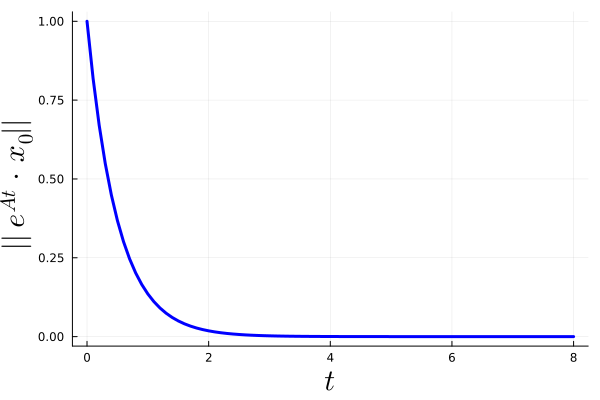
\includegraphics[width=\linewidth]{graphics/Chap09/NormSolutionX0equalsEigenvector1.png}
        % \captionof{figure}{First Image Caption}
        % \label{fig:first_image}
    \end{minipage}
    \hfill
    \begin{minipage}{0.45\columnwidth}
        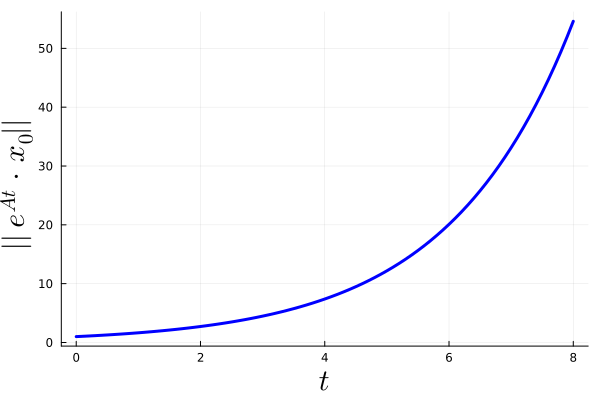
\includegraphics[width=\linewidth]{graphics/Chap09/NormSolutionX0equalsEigenvector2.png}
        % \captionof{figure}{Second Image Caption}
        % \label{fig:second_image}
    \end{minipage}
\end{center}
The image on the left shows $||x(t)||$ decaying like $e^{\lambda_1 t}=e^{-2t}$ and the image on the right shows $||x(t)||$ exploding like $e^{\lambda_2 t} = e^{0.5t}$. This is because, when $x_0=v$, an eigenvector, then $e^{At} \cdot v = e^{\lambda t} v$, and hence, 
$$||e^{A t} \cdot v|| = ||e^{\lambda t} \cdot v|| = |e^{\lambda t}|\, ||v||,$$
which implies for real eigenvalues, 
$$ \lim_{t \to \infty} ||e^{A t} \cdot v|| = \begin{cases}
    0 & \lambda < 0\\
    ||v|| & \lambda = 0\\
    \infty & \lambda >0.
\end{cases}$$
\Qed

\bigskip 

\textcolor{blue}{\bf Our next challenge is to understand what happens in the case of complex eigenvalues and eigenvectors.} Suppose that $A$ is real with complex eigenvalue $\lambda = a + \im \omega$ and corresponding eigenvector, $v = v_R + \im v_I$. From Prop.~\ref{thm:EigenStuffMatrixExponential}, 
$$e^{At} v = e^{\lambda t} v = e^{(a + \im \omega)t} v.$$
Hence, 
$$ ||e^{At} v|| = ||e^{(a + \im \omega)t }v|| = |e^{(a + \im \omega)t }| \cdot ||v|| = |e^{at} \cdot e^{\im \omega t }| \cdot ||v||= |e^{at}| \cdot |e^{\im \omega t}| \cdot ||v|| = e^{at} \cdot |e^{\im \omega t}| \cdot ||v||. $$
By Euler's Formula, 
$$e^{\im \omega t} = \cos( \omega t) + \im \sin( \omega t),$$
and therefore, 
$$|e^{\im \omega t}| = |\cos( \omega t) + \im \sin( \omega t)| = \sqrt{\cos^2( \omega t) + \sin^2( \omega t)} = 1.$$
After all of this, we obtain that
$$||e^{At} v|| = e^{at} ||v||,$$
where $a={{\rm real}(\lambda)}$, the real part of the eigenvalue $\lambda$. 

\vspace*{.8cm} 

\begin{example}
\label{ex:AnalyzeExpAt4Dimensional}
    Use the eigenvectors of $A=\left[
\begin{array}{cccc}
-1.8931 & 11.4911 & 2.8358 & -21.4883 \\
1.9318 & -6.8883 & -0.6626 & 9.1683 \\
-1.4704 & 2.0461 & 0.1305 & -8.2359 \\
1.5956 & -4.4190 & -0.9576 & 5.6509 \\
\end{array}
\right]$ as initial conditions for $\dot{x} = Ax.$ Observe the ``qualitative properties'' of the corresponding solutions. 
\end{example}
\textbf{Solution:}
Let's find the eigenvalues and eigenvectors of $A$.
\begin{lstlisting}[language=Julia,style=mystyle]
# Compute eigenvalues and eigenvectors
A = [-1.89311  11.4911    2.83579   -21.4883
  1.93182  -6.88831  -0.662625    9.16832
 -1.47045   2.04612   0.130518   -8.23588
  1.59557  -4.41903  -0.95763     5.65091]

E=eigen(A)

for k = 1:2
    println("Pair of eigenvalues and vectors")
    display(E.values[(2*k-1):2*k])
    display(E.vectors[:,(2*k-1):2*k])
    println(" ")
end
\end{lstlisting}
\textbf{Output} 
\begin{verbatim}
Pair of eigenvalues and vectors
2-element Vector{ComplexF64}:
 -2.000000213236534 - 1.9999961984135264im
 -2.000000213236534 + 1.9999961984135264im
4×2 Matrix{ComplexF64}:
  -0.314334+0.172478im   -0.314334-0.172478im
 -0.0323151-0.563835im  -0.0323151+0.563835im
  -0.654925-0.0im        -0.654925+0.0im
  -0.121327-0.329915im   -0.121327+0.329915im
 
Pair of eigenvalues and vectors
2-element Vector{ComplexF64}:
 0.5000042132365348 - 2.9999956474834977im
 0.5000042132365348 + 2.9999956474834977im
4×2 Matrix{ComplexF64}:
    0.77073-0.0im          0.77073+0.0im
 -0.0107431+0.313272im  -0.0107431-0.313272im
   0.385818-0.320985im    0.385818+0.320985im
 -0.0406637+0.232767im  -0.0406637-0.232767im
\end{verbatim}
Hence, the eigenvalues 
$$ \lambda_1 = -2-\im2, \quad \lambda_2 =  -2 + \im2, \quad \lambda_3 = 0.5-\im3, \quad \lambda_4 =  0.5 + \im3$$
are complex and respect complex conjugate symmetry, namely, $\lambda_2 = \lambda_1^\ast$ and $\lambda_4 = \lambda_3^\ast$. The corresponding eigenvectors  
$$v_1 = \left[
\begin{array}{r}
 -0.314334+0.172478 \im  \\
 -0.0323151-0.563835 \im \\
  -0.654925-0.000000 \im      \\
  -0.121327-0.329915 \im  
\end{array}
\right], \quad v_2 = 
\left[
\begin{array}{r}
  -0.314334-0.172478 \im\\
 -0.0323151+0.563835 \im\\
    -0.654925+0.000000 \im \\
 -0.121327+0.329915 \im
\end{array}
\right]
$$
$$v_3 = \left[
\begin{array}{r}
    0.77073-0.000000 \im \\
 -0.0107431+0.313272 \im \\
   0.385818-0.320985 \im  \\
 -0.0406637+0.232767 \im 
\end{array}
\right], \quad v_4 = 
\left[
\begin{array}{r}
   0.77073+0.000000 \im \\
 -0.0107431-0.313272 \im \\
   0.385818+0.320985 \im \\
 -0.0406637-0.232767 \im \\
\end{array}
\right]
$$
are also complex and respect complex conjugate symmetry, $v_2 = v_1^\ast$ and $v_4 = v_3^\ast$. \\

We note that ${\rm real}(\lambda_1) = {\rm real}(\lambda_2) =-2< 0$ while ${\rm real}(\lambda_3) = {\rm real}(\lambda_4) =0.5 > 0$. We next compute and plot solutions to $\dot{x}=Ax$, with $x_0 = v_1$ and $x_0 = v_3$. In fact, we are going to plot the norm of each solution, $||e^{At} x_0||$. We show only the code for the first eigenvector as the initial condition.

\begin{lstlisting}[language=Julia,style=mystyle]
# Compute and plot ||x(t) = exp(At)*x0|| for x0 an eigenvector.
using Plots
using LinearAlgebra
using LaTeXStrings

function normSolution(t; A=A, x0=E.vectors[:,1])
    eAt = exp(A*t)
    xt = eAt * x0
    y = norm(xt)
    return y
end

# time values where we compute the solution
t = 0:.1:8

y = normSolution.(t)

p1 = plot(t,y, guidefont = 20, legend = false, xlabel=L"t", ylabel=L"||e^{At}\cdot x_0 ||", lw=3, 
    color=:blue )
\end{lstlisting}
\textbf{Output} 
\begin{center}
    \begin{minipage}{0.45\columnwidth}
        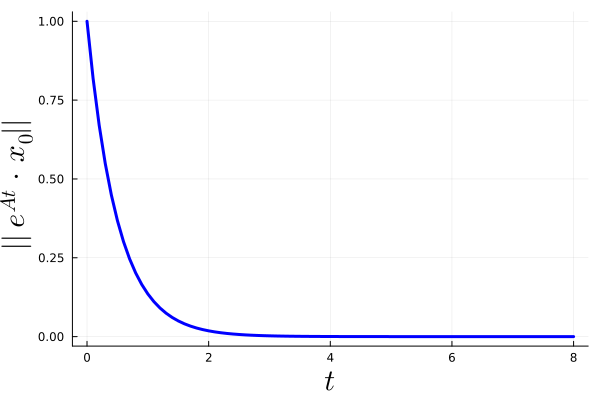
\includegraphics[width=\linewidth]{graphics/Chap09/NormSolutionX0equalsComplexEigenvector1.png}
        % \captionof{figure}{First Image Caption}
        % \label{fig:first_image}
    \end{minipage}
    \hfill
    \begin{minipage}{0.45\columnwidth}
        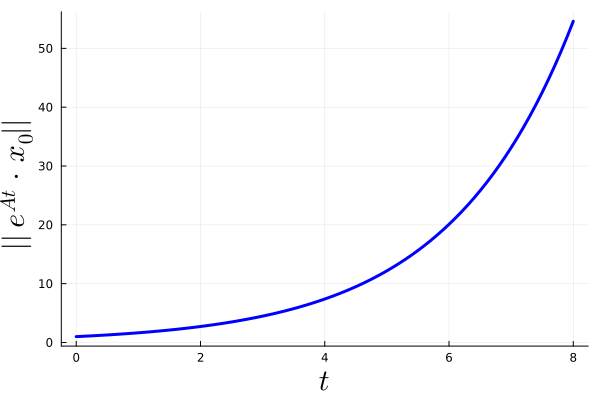
\includegraphics[width=\linewidth]{graphics/Chap09/NormSolutionX0equalsComplexEigenvector2.png}
        % \captionof{figure}{Second Image Caption}
        % \label{fig:second_image}
    \end{minipage}
\end{center}
The image on the left shows $||x(t)||$ decaying like $e^{{\rm real}(\lambda_1) t}=e^{-2t}$ and the image on the right shows $||x(t)||$ exploding like $e^{{\rm real}(\lambda_3) t} = e^{0.5t}$. This is because, when $x_0=v$, an eigenvector, then $e^{At} \cdot v = e^{\lambda t} v$, and hence, 
$$||e^{A t} \cdot v|| = ||e^{\lambda t} \cdot v|| = |e^{\lambda t}| \cdot ||v|| = e^{{\rm real}(\lambda) t} \cdot||v||,$$
which implies for complex eigenvalues, 
$$ \lim_{t \to \infty} ||e^{A t} \cdot v|| = \begin{cases}
    0 & {\rm real}(\lambda) < 0\\
    ||v|| & {\rm real}(\lambda)= 0\\
    \infty & {\rm real}(\lambda) >0.
\end{cases}$$

\bigskip

\begin{center}
\setlength{\fboxrule}{2pt}  % Setting the thickness of the border line
   \fbox{ \parbox{0.9\linewidth}{
   \vspace{.15cm}    
   \textcolor{blue}{\bf What does it mean when the initial condition is a complex vector? That seems very strange!} \textbf{You make a good point.} We've made great progress in understanding the solutions of $\dot{x} = Ax$ for special initial conditions, namely, $x_0$ is an eigenvector of $A$. But yeah, on a real system, we cannot set $x_0$ to a complex value. So, did we just do a bunch of work for nothing? \\

   \textcolor{red}{\bf Hardly.} \textcolor{blue}{\bf However, it does take a bit more Linear Algebra to make sense of our calculations.} 
}
} 
\end{center}

\subsubsection{Complex (scalar) Exponential Functions}


Complex exponentials are a small, yet very powerful generalization of Euler's Formula. If you like to learn from videos, here is \href{https://youtu.be/bDK-gW_P28o}{The MAGIC of Complex Exponentials!} by FiguR3 iT ouT (sic).

\begin{tcolorbox}[colback=mylightblue, title = {\bf Complex Exponetials}, breakable]

\begin{definition}
\label{def:complexExponentials}
 For $a, \omega \in \real$,
\begin{equation}
    e^{(a + \im \omega)t}:= e^{at} \cdot \left( \cos(\omega\, t) + \im \sin(\omega\, t) \right)
\end{equation}
is called a \textbf{complex exponential}. 
\end{definition}


\bigskip

Equivalently, let $z:=a + \im \omega \in \cp$ be a complex number, then $e^{z\, t}$ is a \textbf{complex exponential}.\\

\textbf{Note:} We first encountered a complex exponential in the context of Example~\ref{ex:FirstPeekComplexExponentials}. Complex exponentials arise in the solution of linear ODEs when there are complex eigenvalues.
 \end{tcolorbox}
 
 \bigskip
 
\begin{propColor}{Properties of Complex Exponentials}{PropertiesComplexExponentials}

Complex exponentials are fundamental in various fields of mathematics, engineering, and physics. Below are some of the key properties of complex exponentials, for $a, \omega \in \real$ and
$z:= a + \im \omega \in \cp$:

\begin{enumerate}
\renewcommand{\labelenumi}{(\alph{enumi})}
\setlength{\itemsep}{.2cm}
   
    \item \textbf{Periodicity:} The function $e^{\im \omega t}$ is periodic with period $T = \frac{2\pi}{|\omega|}$, for $\omega \neq 0$.

    \item \textbf{Multiplicative Property:} For any two complex numbers $z_1 = a_1 + \im \omega_1$ and $z_2 = a_2 + \im \omega_2$, the exponential function satisfies $e^{z_1\, t}\cdot e^{z_2 \, t} = e^{\left(z_1 + z_2\right)\, t}$.

    \item \textbf{Inverse:} The inverse of $e^{zt}$ is given by $e^{-zt}$.

    \item \textbf{Differentiation and Integration:} The derivative and antiderivative of $e^{zt}$ with respect to $t$ are: 
    \begin{itemize}
        \item $\frac{d}{dt}e^{zt} = ze^{zt}$ and 

        \item for $z \neq 0$, $\int e^{zt} dt = \frac{1}{z}e^{zt} + C$, where $C$ is the constant of integration.

    \end{itemize}
    \item \textbf{Conjugation:} The complex conjugate of $e^{\left(a + \im \omega \right)t}$ is $e^{\left(a - \im \omega \right)t}$.

    \item \textbf{Magnitude:} The magnitude of $e^{\left(a+ \im \omega \right)t}$ is $|e^{\left(a+ \im \omega \right)\, t}| = e^{at}$, which exhibits exponential growth or decay based on the sign of the real part,  $a$.
\end{enumerate}

\textbf{Note:} These properties make complex exponentials an indispensable tool in the analysis of oscillatory and wave phenomena, signal processing, control theory, and many other areas.

   
\end{propColor}

\subsubsection{Understanding the Roles Played by the Real and Imaginary Parts of Complex Eigenvalues and Eigenvectors}

\bigskip
\begin{propColor}{Real and Imaginary Parts of a Complex Eigenvector as Initial Conditions}{RealImagPartsComplexEvectosAsIC}

Suppose that $A$ is a real $n\times n$ matrix with a complex eigenvalue $\lambda = a + \im \omega$ and corresponding eigenvector $v = v_R + \im v_I$. Then
\begin{equation}
\label{eq:RealSolutionsComplexEigenVectors}
    \begin{aligned}
        e^{At} v_R & = e^{at} \cos(\omega t) v_R -  e^{at} \sin(\omega t) v_I \\
        e^{At} v_I & = e^{at} \sin(\omega t) v_R +  e^{at} \cos(\omega t) v_I. 
    \end{aligned}
\end{equation}

\bigskip

\textbf{Note:} Equation \eqref{eq:RealSolutionsComplexEigenVectors} helps us to see the oscillatory aspect of the solutions of linear ODEs when there are complex eigenvalues. The imaginary part of the eigenvalue, $\omega:={\rm imag}(\lambda)$ sets the (angular) frequency of the oscillation, while the real part of the eigenvalue, $a:={\rm real}(\lambda)$, determines the ``amplification''  or ``attenuation'' factor, depending on $a$ is positive, negative, or zero. \\

When the initial condition is a real eigenvector, the solution of $\dot{x} = Ax$ evolves entirely along the eigenvector via $e^{\lambda t} v$. It is ``living'' in a one-dimensional subspace given by $\spanof{v}$. For a complex eigenvector, when the ODE is initialized at $v_R$ or $v_I$, the solution ``lives'' in a two-dimensional subspace given by $\spanof{v_R, v_I}$. Within that subspace, the solution spirals to the origin if $a <0$, spirals to infinity if $a>0$, and forms a circle if $a=0$. To be able to deduce such detailed information through Linear Algebra is pretty awesome, don't you agree?
    
\end{propColor}
\bigskip

\begin{example} Using our new insights, re-analyze the solutions to $\dot{x}=Ax$ for the matrix in Example~\ref{ex:AnalyzeExpAt4Dimensional}. The key data are
$$A=\left[
\begin{array}{rrrr}
-1.8931 & 11.4911 & 2.8358 & -21.4883 \\
1.9318 & -6.8883 & -0.6626 & 9.1683 \\
-1.4704 & 2.0461 & 0.1305 & -8.2359 \\
1.5956 & -4.4190 & -0.9576 & 5.6509 \\
\end{array}
\right]$$
has eigenvalues,
$$ \lambda_1 = -2-\im2, \quad \lambda_2 = \lambda_1^\ast =  -2 + \im2, \quad \lambda_3 = 0.5-\im3, \quad \lambda_4 =  \lambda_3^\ast = 0.5 + \im3$$
and corresponding eigenvectors  
$$v_1 = \left[
\begin{array}{r}
 -0.3143 \\
-0.0323 \\
-0.6549 \\
-0.1213 \\
\end{array}
\right] + \im \left[
\begin{array}{r}
0.1725 \\
-0.5638 \\
-0.0000 \\
-0.3299 \\
\end{array}
\right], \quad v_2 = v_1^\ast =
\left[
\begin{array}{r}
 -0.3143 \\
-0.0323 \\
-0.6549 \\
-0.1213 \\
\end{array}
\right] - \im \left[
\begin{array}{r}
0.1725 \\
-0.5638 \\
-0.0000 \\
-0.3299 \\
\end{array}
\right]
$$
$$v_3 = \left[
\begin{array}{r}
0.7707 \\
-0.0107 \\
0.3858 \\
-0.0407 \\
\end{array}
\right] + \im \left[
\begin{array}{r}
-0.0000 \\
0.3133 \\
-0.3210 \\
0.2328 \\
\end{array}
\right], \quad v_4 = v_3^\ast=
\left[
\begin{array}{r}
0.7707 \\
-0.0107 \\
0.3858 \\
-0.0407 \\
\end{array}
\right] - \im \left[
\begin{array}{r}
-0.0000 \\
0.3133 \\
-0.3210 \\
0.2328 \\
\end{array}
\right].
$$    
\end{example}


\textbf{Solutions:}
Compute the solution of $e^{At} \cdot v_{R,1}$ and plot its ``projection'' onto $\spanof{v_{R,1}, v_{I,1}}$.
\begin{lstlisting}[language=Julia,style=mystyle]
using LinearAlgebra
using Plots
using LaTeXStrings

A = [-1.89311  11.4911    2.83579   -21.4883
  1.93182  -6.88831  -0.662625    9.16832
 -1.47045   2.04612   0.130518   -8.23588
  1.59557  -4.41903  -0.95763     5.65091]

E=eigen(A)
(lam1, lam2, lam3, lam4) = E.values
(v1, v2, v3, v4) = E.vectors

t = 0.0:0.02:100

# For x0 = real(v1)
x =  exp.(real(lam1)*t).*cos.(imag(lam1)*t)
y = -exp.(real(lam1)*t).*sin.(imag(lam1)*t)

p1 = plot(x, y, guidefont = 15, lw=3, color=:blue, legend=false, 
    aspect_ratio=1, xlabel=L"e^{at}\cos(\omega t) v_R", ylabel=L"-e^{at}\sin(\omega t) v_I")

# mark the initial condition
scatter!([1], [0], markersize=8, color=:red)


display(p1)
\end{lstlisting}

\bigskip
Compute the solution of $e^{At} \cdot v_{I,3}$ and plot its ``projection'' onto $\spanof{v_{R,3}, v_{I,3}}$.
\begin{lstlisting}[language=Julia,style=mystyle]
using LinearAlgebra
using Plots
using LaTeXStrings

A = [-1.89311  11.4911    2.83579   -21.4883
  1.93182  -6.88831  -0.662625    9.16832
 -1.47045   2.04612   0.130518   -8.23588
  1.59557  -4.41903  -0.95763     5.65091]

E=eigen(A)
(lam1, lam2, lam3, lam4) = E.values
(v1, v2, v3, v4) = E.vectors

t = 0.0:0.02:8

# For x0 = imag(v3)
x = exp.(real(lam3)*t).*sin.(imag(lam3)*t)
y = exp.(real(lam3)*t).*cos.(imag(lam3)*t)

p1 = plot(x, y, guidefont = 15, lw=3, color=:red, legend=false, 
    aspect_ratio=1, xlabel=L"e^{at}\sin(\omega t) v_R", ylabel=L"e^{at}\cos(\omega t) v_I")

# mark the initial condition
scatter!([0], [1], markersize=6, color=:blue)

display(p1)
\end{lstlisting}
\textbf{Output} 
\begin{center}
    \begin{minipage}{0.45\columnwidth}
        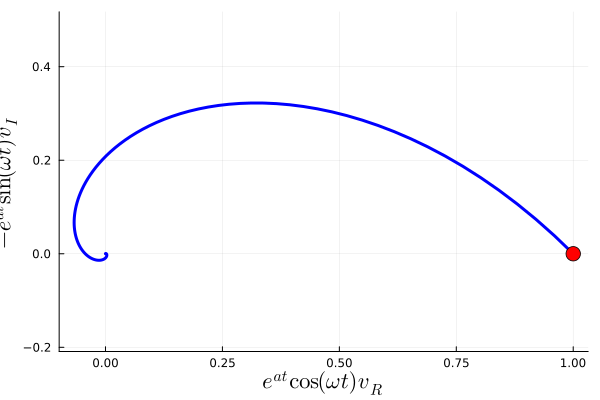
\includegraphics[width=\linewidth]{graphics/Chap09/SpiralInwardPreviousExample.png}
        % \captionof{figure}{First Image Caption}
        % \label{fig:first_image}
    \end{minipage}
    \hfill
    \begin{minipage}{0.45\columnwidth}
        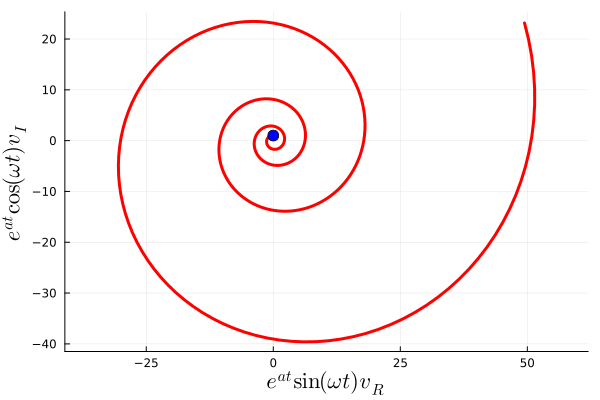
\includegraphics[width=\linewidth]{graphics/Chap09/SpiralOutwardPreviousExample.png}
        % \captionof{figure}{Second Image Caption}
        % \label{fig:second_image}
    \end{minipage}
\end{center}

On the left is the solution of $e^{At}v_{R,1}$, projected onto $\spanof{v_{R,1}, v_{I,1}}$, with the red dot marking the initial condition. $e^{-2t}$ decays so quickly that we cannot see with our eyes very much of the spiral into the origin. On the right is the solution of $e^{At}v_{I,3}$, projected onto $\spanof{v_{R,3}, v_{I,3}}$, with the blue dot marking the initial condition. $e^{0.5t}$ expands slowly enough that we can see it spiral outward to infinity.
\Qed.

\bigskip

Based on the results in this subsection, we understand very well how the solutions to $\dot{x} = Ax$ evolve for initial conditions tied to eigenvectors. The next subsection treats general initial conditions.

\subsection{Exponential Stability of Linear Systems of ODEs with Implications for Nonlinear ODEs}
\label{sec:ExponentialStabilityLTIodes}

\bigskip
\begin{tcolorbox}[colback=mylightblue, title = {\bf Equilibrium Points and Stability Properties}, breakable]
%
Let $A$ be a real $n \times n$ matrix and consider the linear system of ODEs $\dot{x} = Ax$. We specialize Def.~\ref{def:equilibriumPoint} to the case of linear systems.

\begin{definition}
\label{def:EquilibriumPoint}
 $x_e \in \real^n$ is an \textbf{equilibrium point} of $\dot{x} = Ax$ if $Ax_e=0$. Equivalently, the constant vector $\varphi(t, t_0, x_e):=x_e$ is a solution of the ODE. \\
\end{definition}
 \vspace*{.1cm}
\textbf{Note:} For a linear ODE, the origin is always an equilibrium point.


\bigskip

\begin{definition}
\label{def:AsymptoticStability}
 $x_e \in \real^n$ is a \textbf{globally asymptotically stable equilibrium point} of $\dot{x} = Ax$ if for all $x_0\in  \real$,
 $$\lim_{t \to \infty} e^{At} x_0 = 0.$$
\end{definition}
 \bigskip
\begin{definition}
\label{def:ExponentialStability}
 $x_e \in \real^n$ is a \textbf{globally exponentially stable equilibrium point} of $\dot{x} = Ax$ if there exist $\kappa >0$ and $\gamma< \infty$ such that, for all $x_0\in  \real$, 
 $$ ||e^{At} x_0|| \le \gamma\cdot e^{-\kappa t} \cdot ||x_0||. $$
\end{definition}
\bigskip
\textbf{Note:}  For a linear system of ODEs, Global \textbf{exponential} stability of an equilibrium point and global \textbf{asymptotic} stability of an equilibrium point are equivalent concepts. For a nonlinear system of ODEs, they are different notions of stability. In this course, understanding that each notion implies that solutions converge to zero as time marches to infinity is enough. The rate at which the convergence takes place is less relevant. 
\end{tcolorbox}

\bigskip
\begin{center}
\setlength{\fboxrule}{2pt}  % Setting the thickness of the border line
   \fbox{ \parbox{0.9\linewidth}{
   \vspace{.15cm}    
   \textcolor{blue}{\bf We laid the seeds for guessing that the \textcolor{red}{\bf eigenvalues} provide all the information needed to check for asymptotic stability. The \textcolor{red}{\bf eigenvectors} were present because, when used as an initial condition, the solution to a linear ODE is very simple, $\bm{e^{At}\cdot v = e^{\lambda t} v}$. } 
}
} 
\end{center}

\bigskip
\begin{propColor}{Exponential Stability of Linear Systems of ODEs}{ExpStabilityLinearSystems}
Let $A$ be a real $n \times n$ matrix with eigenvalues $\lambda_1, \lambda_2, \ldots, \lambda_n$, and consider the linear system of ODEs,
$$\dot{x} = Ax.$$
If ${\rm real}(\lambda_i)< 0$ for $1 \le i \le n$ (aka, the real parts of all eigenvalues are negative), then the \textbf{origin} is globally exponentially stable.  

\bigskip
\textbf{Note:} The proof is given in Chapter~\ref{sec:ODEproofs} for the case of distinct eigenvalues. The general case is part of EECS 560 Linear Systems and uses something called a \href{https://en.wikipedia.org/wiki/Jordan_normal_form}{Jordan Normal Form} for square matrices. While it's an awesome thing to know, saving a few things for grad school is okay.
\end{propColor}

\bigskip

\begin{example} Determine if the origin is a globally exponentially stable equilibrium point for the following linear systems of ODEs.

 \begin{enumerate}
\renewcommand{\labelenumi}{(\alph{enumi})}
\setlength{\itemsep}{.2cm}

\item Consider the mass-spring-damper system in Example~\ref{ex:MassSpringDamperNoGravity}. When $m = 5$ kg, $k = 2$ N/m, and $b = 3$ Ns/m (Newton seconds per meter), the model becomes
$$\dot{x} = \left[
\begin{array}{rr}
0.0000 & 1.0000 \\
-0.4000 & -0.6000 \\
\end{array}
\right] \cdot x.$$


\item Consider the RLC network in Example~\ref{ex:RLCcircuit}. For a consumer-grade RLC circuit in an older WiFi radio receiver, where discrete circuit elements were still used, typical component values might be:
\begin{itemize}
    \item (R) 10 kilo-ohms (k$\Omega$)
    \item (L) 20 nanohenries (nH)
    \item (C) 10 nanofarads (nF),
\end{itemize}
yielding $\dot{x} = A x$, with 
$$A=\left[
\begin{array}{rr}
0.0000e+00 & 1.0000e+08 \\
-5.0000e-01 & -5.0000e+11 \\
\end{array}
\right].$$ 
\end{enumerate}
\end{example}
\textbf{Solutions:}
 \begin{enumerate}
\renewcommand{\labelenumi}{(\alph{enumi})}
\setlength{\itemsep}{.2cm}

\item Mass-spring-damper system: \Ans \quad  The origin is globally exponentially stable because the eigenvalues all have negative real parts. 

\begin{lstlisting}[language=Julia,style=mystyle]
using LinearAlgebra
# Mass spring damper system
m = 5 # kg
k = 2 # N/m
b = 3 # Ns/m (Newton seconds per meter)
A = [0 1; -k/m -b/m]
E = eigen(A)
\end{lstlisting}
\textbf{Output} 
\begin{verbatim}
Eigen{ComplexF64, ComplexF64, Matrix{ComplexF64}, Vector{ComplexF64}}
values:
2-element Vector{ComplexF64}:
 -0.29999999999999993 - 0.5567764362830022im
 -0.29999999999999993 + 0.5567764362830022im
 
vectors:
2×2 Matrix{ComplexF64}:
  0.845154-0.0im        0.845154+0.0im
 -0.253546-0.470562im  -0.253546+0.470562im
\end{verbatim}



\item RLC network:  \Ans \quad  The origin is globally exponentially stable because the eigenvalues all have negative real parts. 

\begin{lstlisting}[language=Julia,style=mystyle]
using LinearAlgebra
# RLC Circuit
R = 10e3 # ohms
L = 20e-9 # Henries
C = 10e-9 # farads
A = [0 1/C; -C/L -R/L]
E = eigen(A)
\end{lstlisting}
\textbf{Output} 
\begin{verbatim}
Eigen{Float64, Float64, Matrix{Float64}, Vector{Float64}}
values:
2-element Vector{Float64}:
 -4.999999999999999e11
 -0.0001220703125
 
vectors:
2×2 Matrix{Float64}:
 -0.0002   1.0
  1.0     -1.0e-12
\end{verbatim}
\end{enumerate}

\Qed

\bigskip
\begin{example} 
\label{ex:RandomInitialConditionMassSpringDamper}
Take a random initial condition for the mass-spring-damper system and plot the norm of its solution.    
\end{example}
\textbf{Solution:}
\begin{lstlisting}[language=Julia,style=mystyle]
# Take a random initial condition for the mass-spring-damper system and plot the norm of its solution.   
using Plots
using LinearAlgebra
using Random
using LaTeXStrings

# Mass spring damper system
m = 5 # kg
k = 2 # N/m
b = 3 # Ns/m (Newton seconds per meter)
A = [0 1; -k/m -b/m]


Random.seed!(543210)
x0 = randn(2,1); display(x0)
function normSolution(t; A=A, x0=x0)
    eAt = exp(A*t)
    xt = eAt * x0
    y = norm(xt)
    return y
end

# time values where we compute the solution
t = 0:0.01:20

y = normSolution.(t)

p1 = plot(t,y, guidefont = 20, legend = false, xlabel=L"t", ylabel=L"||e^{At}\cdot x_0 ||", lw=3, 
    color=:blue )
\end{lstlisting}
\textbf{Output} 
\begin{verbatim}
2×1 Matrix{Float64}:
 -0.9072986899852817
  0.7151631134658601
\end{verbatim}
Because the eigenvalues are complex, we see oscillation in the norm as the solution decays to the origin, $x_e=[0; 0]$.
\begin{center}
    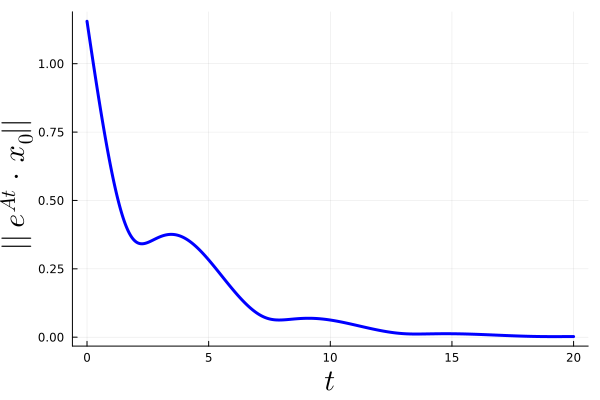
\includegraphics[width=0.6\columnwidth]{graphics/Chap09/NormSolutionX0randomMassSpringDamper.png}
\end{center}

\Qed
\bigskip


\begin{example} Determine if the origin is a globally exponentially stable equilibrium point for the linearized model of the 2-link robot arm, for the (a) upward equilibrium and (b) downward equilibrium. We chose the 2-link arm so that we need to do everything from scratch:
\begin{itemize}
    \item build the dynamic model,
    \item compute the linearization for each of the equilibria, and
    \item evaluate the eigenvalues. 
\end{itemize}
In addition, for a random initial condition, compute solutions to each of the linearized models.
\end{example}

\textbf{Solutions: }

\begin{enumerate}
\renewcommand{\labelenumi}{(\alph{enumi})}
\setlength{\itemsep}{.2cm}
\item Upward equilibrium. \Ans \quad The origin is not exponentially stable. There are four real eigenvalues, of which two are positive.

\item Downward equilibrium. \Ans \quad The origin is not exponentially stable.  There are four purely imaginary eigenvalues, meaning their real part is identically zero.
\end{enumerate}

\bigskip
\begin{center}
    \begin{minipage}{0.45\columnwidth}
        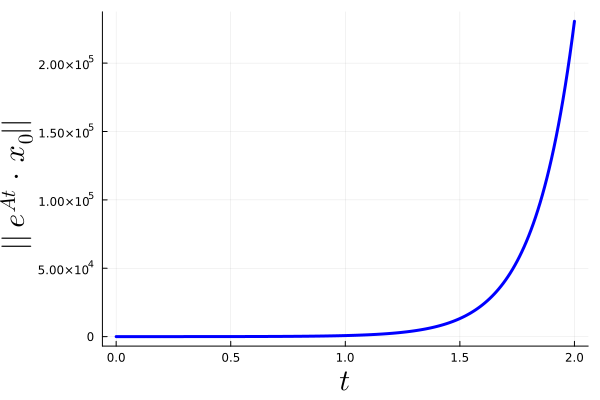
\includegraphics[width=\linewidth]{graphics/Chap09/NormSolutionX0randomUpwardEquilibrium2LinkArm.png}
        % \captionof{figure}{First Image Caption}
        % \label{fig:first_image}
    \end{minipage}
    \hfill
    \begin{minipage}{0.45\columnwidth}
        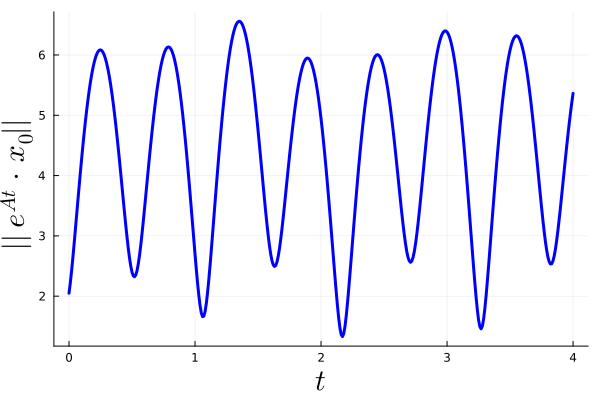
\includegraphics[width=\linewidth]{graphics/Chap09/NormSolutionX0randomDownwardEquilibrium2LinkArm.png}
        % \captionof{figure}{Second Image Caption}
        % \label{fig:second_image}
    \end{minipage}
\end{center}

\bigskip
Using Lagrange's Method, we obtain,
\begin{lstlisting}[language=Julia,style=mystyle]
function dyn_mod_2LinkManipulator(q, dq)
# DYN_MOD_2LINKMANIPULATOR
# 2023-12-05 14:45:06
#
# Author: Grizzle
#
# Model NOTATION: D(q)ddq + C(q,dq)*dq + G(q) = B*tau 
# The Robot Equations: From Lagrange's Equations of Motion
#
g, L1, L2, m1, m2 = modelParameters()
#
# Variable names for the model
q1, q2= q 
dq1, dq2 = dq
#
D = zeros(2, 2)
  D[1, 1] = L1^2*m1 + m2*(L1^2 + 2*L1*L2*cos(q2) + L2^2)
  D[1, 2] = L2*m2*(L1*cos(q2) + L2)
  D[2, 1] = L2*m2*(L1*cos(q2) + L2)
  D[2, 2] = L2^2*m2
#
C = zeros(2, 2)
  C[1, 1] = -L1*L2*dq2*m2*sin(q2)
  C[1, 2] = -L1*L2*m2*(dq1 + dq2)*sin(q2)
  C[2, 1] = L1*L2*dq1*m2*sin(q2)
  C[2, 2] = 0.0
#
G = zeros(2)
  G[1] = g*m2*(L1*cos(q1) + L2*cos(q1 + q2)) + L1*g*m1*cos(q1)
  G[2] = L2*g*m2*cos(q1 + q2)
#
B = zeros(2, 2)
  B[1, 1] = 1
  B[2, 2] = 1
#
JacG = zeros(2, 2)
  JacG[1, 1] = g*m2*(-L1*sin(q1) - L2*sin(q1 + q2)) - L1*g*m1*sin(q1)
  JacG[1, 2] = -L2*g*m2*sin(q1 + q2)
  JacG[2, 1] = -L2*g*m2*sin(q1 + q2)
  JacG[2, 2] = -L2*g*m2*sin(q1 + q2)
#
  return (D=D, C=C, G=G, B=B, JacG=JacG)
end
\end{lstlisting}


\bigskip
\textbf{Upward Equilibrium}

\begin{lstlisting}[language=Julia,style=mystyle]
# Linear Model for the 2-link Manipulator
#
# bring the model into the workspace for later use
include("dyn_mod_2LinkManipulator.jl") 

#Build a function to define the parameters of the model

function modelParameters()
    g = 9.81 # m/s^2
    L1 = 1 # m
    L2 = 0.7
    m1 = 15 # kg
    m2 = 10   
    return g, L1, L2, m1, m2
end

# Set equilibirum Point
if false
    qe = [-pi/2, 0] #downward
else
    qe = [pi/2, 0] # upward
end

F = dyn_mod_2LinkManipulator(qe, 0*qe)
D = F.D; 
println("D matrix"); display(D)
JacG = F.JacG; 
println("JacG matrix"); display(JacG)

# build the linearized model about the give equilibrium point
A21 = -D\JacG; A21 = cleanUp(A21); 
println("A21 matrix"); display(A21)
n, ~ = size(A21)
A = [zeros(n,n) I(n); A21 zeros(n,n)]; 
println("A matrix"); display(A)
        
# Compute eigenvalues
E = eigen(A)        
\end{lstlisting}
\textbf{Output} 
\begin{verbatim}
D matrix
2×2 Matrix{Float64}:
 43.9  11.9
 11.9   4.9
 
JacG matrix
2×2 Matrix{Float64}:
 -313.92  -68.67
  -68.67  -68.67
  
A21 matrix
2×2 Matrix{Float64}:
  9.81  -6.54
 -9.81  29.8971
 
A matrix
4×4 Matrix{Float64}:
  0.0    0.0     1.0  0.0
  0.0    0.0     0.0  1.0
  9.81  -6.54    0.0  0.0
 -9.81  29.8971  0.0  0.0
 
Eigen{Float64, Float64, Matrix{Float64}, Vector{Float64}}
values:
4-element Vector{Float64}:
 -5.718391382198321
 -2.647100840002673
  2.647100840002673
  5.71839138219832
  
vectors:
4×4 Matrix{Float64}:
 -0.0473235  -0.324822  0.324822   0.0473235
  0.165632   -0.139209  0.139209  -0.165632
  0.270614    0.859836  0.859836   0.270614
 -0.947151    0.368501  0.368501  -0.947151
\end{verbatim}

\bigskip
\textbf{Downward Equilibrium}
\begin{lstlisting}[language=Julia,style=mystyle]
# Linear Model for the 2-link Manipulator
#
# bring the model into the workspace for later use
include("dyn_mod_2LinkManipulator.jl") 

#Build a function to define the parameters of the model

function modelParameters()
    g = 9.81 # m/s^2
    L1 = 1 # m
    L2 = 0.7
    m1 = 15 # kg
    m2 = 10   
    return g, L1, L2, m1, m2
end

# Set equilibirum Point
if true
    qe = [-pi/2, 0] #downward
else
    qe = [pi/2, 0] # upward
end

F = dyn_mod_2LinkManipulator(qe, 0*qe)
D = F.D; 
println("D matrix"); display(D)
JacG = F.JacG; 
println("JacG matrix"); display(JacG)

# build the linearized model about the given equilibrium point
A21 = -D\JacG; A21 = cleanUp(A21); 
println("A21 matrix"); display(A21)
n, ~ = size(A21)
A = [zeros(n,n) I(n); A21 zeros(n,n)]; 
println("A matrix"); display(A)
        
# Compute eigenvalues
E = eigen(A)  
\end{lstlisting}
\textbf{Output} 
\begin{verbatim}
D matrix
2×2 Matrix{Float64}:
 43.9  11.9
 11.9   4.9
 
JacG matrix
2×2 Matrix{Float64}:
 313.92  68.67
  68.67  68.67

A21 matrix
2×2 Matrix{Float64}:
 -9.81    6.54
  9.81  -29.8971
  
A matrix
4×4 Matrix{Float64}:
  0.0     0.0     1.0  0.0
  0.0     0.0     0.0  1.0
 -9.81    6.54    0.0  0.0
  9.81  -29.8971  0.0  0.0
  
Eigen{ComplexF64, ComplexF64, Matrix{ComplexF64}, Vector{ComplexF64}}
values:
4-element Vector{ComplexF64}:
 2.2204460492502973e-16 - 2.6471008400026728im
 2.2204460492502973e-16 + 2.6471008400026728im
  3.945433097643709e-16 - 5.718391382198318im
  3.945433097643709e-16 + 5.718391382198318im
  
vectors:
4×4 Matrix{ComplexF64}:
  6.06496e-17-0.324822im     …  1.65597e-17-0.0473235im
 -2.13366e-17-0.139209im        2.56542e-17+0.165632im
    -0.859836-0.0im                0.270614+2.991e-17im
    -0.368501+2.66706e-16im       -0.947151+0.0im
\end{verbatim}
\bigskip
Solutions are computed using the same code as in Example~\ref{ex:RandomInitialConditionMassSpringDamper}.

\Qed

\bigskip
\begin{center}
\setlength{\fboxrule}{2pt}  % Setting the thickness of the border line
   \fbox{ \parbox{0.9\linewidth}{
   \vspace{.15cm}    
   \textcolor{blue}{\bf This next example illustrates the power of feedback control. The particular ``type'' of controller employed is linear state-variable feedback. The example uses material from Michigan's EECS 560 \textit{Linear Systems Theory} to design the feedback controller and illustrates two important points:} \textbf{
   \begin{itemize}
       \item an unstable equilibrium point can often be made into an exponentially stable equilibrium point with a properly designed feedback controller; and 
       \item global exponential stability of a linearized model about an equilibrium point implies local exponential stability of the nonlinear model about the same equilibrium point.
   \end{itemize}} 
   Many feedback controllers in engineering practice are designed on the basis of these two facts; the second fact is proved in Michigan's EECS 562 \textit{Nonlinear Systems and Control}. 
}
} 
\end{center}
\bigskip


\begin{example} 
\label{ex:StabilizeNonlinear2LinkRobotArmUpwardEquilibrium}
Consider the following linearized model of the 2-link robot arm about the upward equilibrium, where motors (aka, actuators) have been added to the two joints, 
\begin{equation}
\delta \dot{x} = \underbrace{\left[
\begin{array}{rrrr}
0.000 & 0.000 & 1.000 & 0.000 \\
0.000 & 0.000 & 0.000 & 1.000 \\
9.810 & -6.540 & 0.000 & 0.000 \\
-9.810 & 29.897 & 0.000 & 0.000 \\
\end{array}
\right]}_{A} \delta x + \underbrace{\left[
\begin{array}{rr}
0.000 & 0.000 \\
0.000 & 0.000 \\
0.067 & -0.162 \\
-0.162 & 0.597 \\
\end{array}
\right]}_{B} \delta \tau,
\end{equation}
where $ \delta x: = \underbrace{\left[\begin{array}{r}
x_1 \\
x_2 \\
x_3 \\
x_4\\
\end{array}
\right]}_{x}- \underbrace{\left[
\begin{array}{r}
1.571 \\
0.000 \\
0.000 \\
0.000 \\
\end{array}
\right]}_{x_e} $ and  $\delta \tau := \underbrace{\left[\begin{array}{r}
\tau_1 \\
\tau_2 \\
\end{array}
\right]}_{\tau} - \underbrace{\left[\begin{array}{r}
0\\
0 \\
\end{array}
\right]}_{\tau_e} $. $\tau_e$ is the value of the motor torque at the equilibrium point. In this case, it equals $0_{2 \times 1}$, because no torque is required at the equilibrium.\\


Because motors have been attached to both joints (aka, the joints are now actuated), we have the possibility to apply motor torques $(\tau_1, \tau_2)$ to render the upward equilibrium exponentially stable. When the applied motor torques are made a linear function of the states of the model, this is called \textbf{linear state-variable feedback control}: $\tau = -K \cdot (x - x_e) = -K \delta x$,
where, in our case, $K$ is a $2 \times 4$ matrix of \textbf{controller gains}. Using methods from Michigan's EECS 560, a linear state-variable feedback controller has been designed for you,
\begin{equation}
\delta \tau = - \underbrace{\left[
\begin{array}{rrrr}
357.820 & 80.570 & 62.084 & 16.829 \\
80.570 & 73.570 & 16.829 & 6.930 \\
\end{array}
\right]}_{K} \delta x.
\end{equation}
Your tasks are:

\begin{enumerate}
\renewcommand{\labelenumi}{(\alph{enumi})}
\setlength{\itemsep}{.2cm}
\item Determine the eigenvalues of the closed-loop linearized system.
\item Apply the linear state-variable feedback to the nonlinear model of the 2-link robot arm and produce a simulation for 
$x_0 = 
\left[
\begin{array}{r}
0.785 \\
-0.785 \\
0.000 \\
0.000 \\
\end{array}
\right]
$, which has the base link at $\frac{\pi}{4}$ from the horizontal and the second link at $-\frac{\pi}{4}$ from the base link.
\end{enumerate}
\textcolor{blue}{\bf Will it topple over, or will it stand up and balance?} 

\end{example}
\textbf{Solution:} \Ans Here is a \href{https://www.dropbox.com/scl/fi/bnci6n1rkczpwj241nyw2/inverted2LinkRobotArm.gif?rlkey=do5u9duymxhdzekj4q4xejd8y&dl=0}{GIF} generated from a simulation of the nonlinear 2-link robot arm, using the linear feedback controller. See the \textcolor{red}{\bf Caveat} below. 

\begin{center}
    \begin{minipage}{0.45\columnwidth}
        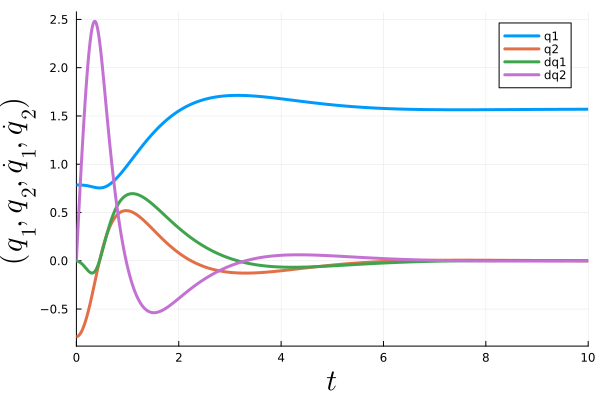
\includegraphics[width=\linewidth]{graphics/Chap09/2LinkManipulatorSimulationClosedLoopStates.png}
        % \captionof{figure}{First Image Caption}
        % \label{fig:first_image}
    \end{minipage}
    \hfill
    \begin{minipage}{0.45\columnwidth}
        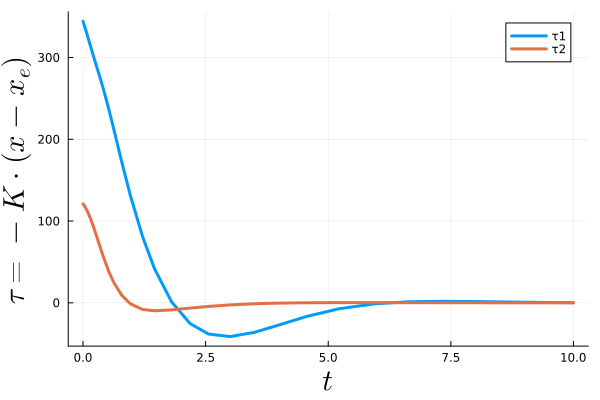
\includegraphics[width=\linewidth]{graphics/Chap09/2LinkManipulatorSimulationClosedLoopStatesControlSignals.png}
        % \captionof{figure}{Second Image Caption}
        % \label{fig:second_image}
    \end{minipage}
\end{center}
 \bigskip

 \textcolor{red}{\bf Caveat:} The model we have chosen is particularly simple because (1) each joint of the robot arm is actuated, and (2), we have assumed the motors can produce as much torque as the controller demands of them. Not all robots have as many actuators as joints and real motors have limitations. Chapter~\ref{chap:LaplaceTransformFeedbackControl} will dig into these issues. For now, we ignore them and simply marvel at the fact that we were able to balance the arm in the inverted position. The BallBot used in ROB 311 \textit{How to Build Robots and Make them Move} is an \textbf{underactuated robot}, meaning it has fewer actuators than it has position variables. We will confront the balance control of such super-challenging robots in Chapter~\ref{chap:LaplaceTransformFeedbackControl}. You may recall the Segway from Project 3 in ROB 101 \textit{Computational Linear Algebra}; it too is an underactuated mobile robot.

  \bigskip

  \subsubsection{Build the linearized model:}
\begin{lstlisting}[language=Julia,style=mystyle]
# Linear Model for the 2-link Manipulator
#
# bring the model into the workspace for later use
include("dyn_mod_2LinkManipulator.jl") 

#Build a function to define the parameters of the model

function modelParameters()
    g = 9.81 # m/s^2
    L1 = 1 # m
    L2 = 0.7
    m1 = 15 # kg
    m2 = 10   
    return g, L1, L2, m1, m2
end

# Set equilibirum Point
if false
    qe = [-pi/2, 0] #downward
else
    qe = [pi/2, 0] # upward
end

F = dyn_mod_2LinkManipulator(qe, 0*qe)
D = F.D; 
JacG = F.JacG; 
B = F.B; 

# build the linearized model about the given equilibrium point
A21 = -D\JacG; A21 = cleanUp(A21); 
n, ~ = size(A21)
A = [zeros(n,n) I(n); A21 zeros(n,n)];
B = [zeros(n,n); F.D \ B];
display(A)
display(B)
\end{lstlisting}
\textbf{Output} 
\begin{verbatim}
4×4 Matrix{Float64}:
  0.0    0.0     1.0  0.0
  0.0    0.0     0.0  1.0
  9.81  -6.54    0.0  0.0
 -9.81  29.8971  0.0  0.0
 
4×2 Matrix{Float64}:
  0.0         0.0
  0.0         0.0
  0.0666667  -0.161905
 -0.161905    0.597279
\end{verbatim}

\subsubsection{Using the given feedback gain matrix, K, compute the closed-loop eigenvalues}
Consider a linear model $\dot{x} = Ax + B u$, where $u$ is the traditional notation for the control input in the Feedback Control Community. Suppose that a linear feedback $u = -Kx$ is applied to the system. Then we have
\begin{align*}
    \dot{x} &= Ax + Bu \\
    &= Ax + B\cdot \left( -Kx \right) ~~(\text{substitute in the feedback}) \\
    & = \left( A-B\cdot K\right) x ~~(\text{algebra}).
\end{align*}
Hence, the eigenvalues of $A-B\cdot K$ determine the asymptotic stability of the closed-loop system.
 \bigskip

\begin{lstlisting}[language=Julia,style=mystyle]
K=[
 357.82  80.57  62.084   16.8291
  80.57  73.57  16.8291   6.92965
]
eigen(A-B*K)
\end{lstlisting}
\textbf{Output} 
\begin{verbatim}
Eigen{ComplexF64, ComplexF64, Matrix{ComplexF64}, Vector{ComplexF64}}
values:
4-element Vector{ComplexF64}:
 -0.7071159639815681 - 0.7070975982722726im
 -0.7071159639815681 + 0.7070975982722726im
 -0.7071061788755746 - 0.7071073834970084im
 -0.7071061788755746 + 0.7071073834970084im
 
vectors:
4×4 Matrix{ComplexF64}:
 -0.223141-2.18102e-11im  -0.223141+2.18102e-11im  …  -0.233087-5.00046e-11im
  0.670976-0.0im           0.670976+0.0im             -0.667586+0.0im
  0.157786+0.157782im      0.157786-0.157782im         0.164817-0.164818im
 -0.474458-0.474445im     -0.474458+0.474445im         0.472054-0.472055im
\end{verbatim}
The closed-loop eigenvalues have been placed at $-\frac{\sqrt{2}}{2} \pm \im \frac{\sqrt{2}}{2}$. Hence, the upright equilibrium is now globally exponentially stable for the linearized model.

\subsubsection{Simulate the Nonlinear Closed-loop System}

\begin{lstlisting}[language=Julia,style=mystyle]
# Import useful packages
using DifferentialEquations
using Plots 
using LaTeXStrings
using LinearAlgebra # for the backslash command
gr()


# bring the model into the workspace for later use
include("dyn_mod_2LinkManipulator.jl") 

# Parameters for the Feedback controller

struct Params
    qe::Vector{Float64}      # equilibrium point
    K ::Matrix{Float64}      # LQR Feedback gain matrix
end
# Initialize the Params structure with specific values
params = Params(qe, K)


# define the ODE dx/dt = f(x,t)
#
# the parameters are passed via modelParameters() in the
# function dyn_mod_2LinkManipulator(q, dq)
#
function f(x,params,t)
    n = floor(Int, length(x) / 2) # In Julia n/2 is a Float64
    q = x[1:n]
    dq = x[n+1:end]
    K = params.K 
    qe = params.qe
    xe = [qe; 0*qe]
    tau = -K*(x-xe)
    model = dyn_mod_2LinkManipulator(q, dq)     
    dx1 = dq
    dx2 = (model.D) \ ( -model.C*dq-model.G+model.B*tau) # note the use of backslash
    dx=[dx1;dx2]
    return dx
end

# Set the initial condition as a vector
x0= [qe;0*qe] - [pi/4; pi/4; 0; 0]

# Set the time interval
T = (0.0, 10) 

# Setup the ODE problem with out-of-place function
problem = ODEProblem{false}(f, x0, T, params)

# solve the ODE problem using the Runge Kutta Tsitouras 5/4 Integrator
 sol = solve(problem, Tsit5());
#sol = solve(problem, Vern9());


# plot the solution
p1 = plot(sol, lw=3, guidefont=20, xlabel=L"t", ylabel=L"(q_1, q_2, \dot{q}_1, \dot{q}_2)", 
    label=["q1" "q2" "dq1" "dq2"], legend=:topright)
display(p1)


# Extract state variables from the solution
x_sol = Array(sol)

# Preallocate the array for control signals
tau_sol = zeros(2,size(x_sol,2))

# Define terms in the feedback controller
K = params.K 
qe = params.qe
xe = [qe; 0*qe]

# Compute the control signal at each time step
for i in 1:size(x_sol, 2)
    x = x_sol[:, i]
    tau_sol[:, i] = -K * (x - xe)
end

# Plot the control signal
p2 = plot(sol.t, tau_sol', lw=3, guidefont=20, xlabel=L"t", ylabel=L"\tau = -K \cdot(x-x_e)", 
          label=["tau_1" "tau_2"], legend=:topright)
display(p2)
\end{lstlisting}
\textbf{Output} 
The plots were moved to the beginning of the solution.

\subsubsection{Make a GIF}

\begin{lstlisting}[language=Julia,style=mystyle]
using Plots

# Robot parameters
g, L1, L2, m1, m2 = modelParameters()

# Function to calculate forwardKinematics
function forwardKinematics(q1, q2)
    p1 = L1 * [cos(q1), sin(q1)]
    p2 = p1 + L2 * [cos(q1 + q2), sin(q1 + q2)]
    return p1, p2
end

# Extract q1 and q2 from the solution
q1_vals = x_sol[1, :]
q2_vals = x_sol[2, :]

# Create a plot for each time step and save as a GIF
anim = @animate for i in 1:length(q1_vals)
    p1, p2 = forwardKinematics(q1_vals[i], q2_vals[i])
    plot([0, p1[1], p2[1]], [0, p1[2], p2[2]], legend=false, lw=3, color=:blue,
        xlims=(-(L1+L2), L1+L2), ylims=(-(L1+L2)/10, 1.1*(L1+L2)), aspect_ratio=1)
    scatter!([p1[1]], [p1[2]], color=:red, markersize = m1)
    scatter!([p2[1]], [p2[2]], color=:red, markersize = m2)
    scatter!([0.0], [0.0], color=:black, markersize = m1+m2)
end

gif(anim, "inverted2LinkRobotArm.gif", fps = 10)
\end{lstlisting}
\textbf{Output} 
Here is the \href{https://www.dropbox.com/scl/fi/ftjk3moa019basvk4zv8o/inverted2LinkRobotArmDeliberatelyDestabilized.gif?rlkey=ledhzmp2u06kv1p15y839v9w9&dl=0}{GIF}; it is the same as the one provided at the beginning of the solution. \textbf{Just Kidding!} The GIF shows what happens if one messes up the SIGN on the feedback controller gain. Instead of implementing $u = -K x$, the sign was flipped and the feedback implemented as $u=Kx$. The resulting eigenvalues are 
$$\lambda_{1,...,4} = \left[
\begin{array}{r}
-7.472 \\
-3.232 \\
4.646 \\
8.886 \\
\end{array}
\right].$$
In the linearized model, the states head off to infinity (in norm). In the nonlinear model, there are rotational joints, where arithmetic modulo $2 \pi$ comes into play ... at least in theory. In most real robots, the limbs cannot make a full rotation without having a self-collision with another part of the robot, or, hitting a hard stop that has been installed for safety reasons. Hitting the hard stop makes a loud noise and usually breaks something. If you are fortunate enough to be working on a modern commercial robot, the system likely has a piece of software supervising the commands to the robot joints and it will shut down the robot before anything dangerous has happened.

\bigskip
\begin{center}
\setlength{\fboxrule}{2pt}  % Setting the thickness of the border line
   \fbox{ \parbox{0.9\linewidth}{
   \vspace{.15cm}    
   \textcolor{blue}{\bf In a feedback loop, if the sign on the gains is wrong, the closed-loop system is usually toast. Many other things can cause a feedback controller to fail, but getting the sign wrong is the most egregious error. } It seems like a silly mistake, one nearly impossible to make, but all it takes is one miscommunication with a team member for it to happen, as your author experienced early in his career. And it was on me as the lead control system designer. Talk about \href{https://www.youtube.com/watch?v=EoltX9mF5Dc}{egg on your face} ... it's like putting your hand on a hot stove ... you do not repeat the error.
   \vspace{.15cm}  
}
} 
\end{center}
  
 \Qed

\section*{Julia Packages for Feedback Control Design}

\begin{itemize}
    \item \textbf{ControlSystems.jl:} A comprehensive control systems toolbox in Julia for system modeling, analysis, controller design, and simulation. Supports state-space and frequency domain methods.
    \item \textbf{RobustAndOptimalControl.jl:} Focuses on robust and optimal control, extending the capabilities of ControlSystems.jl. Includes advanced techniques like H-infinity and robust control.
    \item \textbf{Systems.jl:} Offers tools for modeling, simulation, and analysis of dynamical systems, essential in control design.
    \item \textbf{LCMCore.jl:} Useful for control system applications, particularly in communication between system components.
\end{itemize}


% \section{Linearization of a Nonlinear ODE about an Equilibrium Point}

% \begin{itemize}
%     \item What is an equilibrium point
%     \item $A:= \frac{\partial f(x)}{\partial x}$
%     \item Local exponential stability
% \end{itemize}

\section{When in a Bind, Euler's Method is Always There for You}

% \href{https://youtu.be/v-pbGAts_Fg}{Euler's Method scene in Hidden Figures}
% \href{https://youtu.be/gdxYsVniOYo}{Katherine Johnson and Euler's Method} by the UCLA Modeling Class.

Yes, him again, the Einstein of his era! Euler's Method is one of the most fundamental and historically significant algorithms for computing numerical solutions to ODEs. Named after the uber-prolific Swiss mathematician Leonhard Euler, this method provides a straightforward yet powerful approach for approximating solutions to ODEs, a cornerstone in mathematical modeling of natural and engineered processes. 
Euler's Method is particularly renowned for its simplicity and ease of implementation, making it an excellent starting point for understanding numerical techniques in differential equations. At its core, the method transforms the often daunting task of solving complex ODEs into a \texttt{for loop}. This is achieved by approximating the slope of the solution curve at a series of points, thereby constructing a piecewise linear approximation to the solution. While Euler's Method may not boast the precision of more advanced techniques, such as \href{https://docs.sciml.ai/DiffEqDocs/stable/solvers/ode_solve/#Explicit-Runge-Kutta-Methods}{Runge-Kutta} methods, its conceptual clarity offers invaluable insights into the behavior of differential equations. It serves as a stepping stone to more sophisticated algorithms, providing a foundational understanding of how numerical integration can bridge the gap between analytical mathematics and practical computation.



\bigskip


\begin{funColor}{Euler's Method and Katherine Johnson, an American Hero!}{KatherineJohnson}

\textbf{A super interesting video:} \href{https://youtu.be/gdxYsVniOYo}{Katherine Johnson and Euler's Method} by the UCLA Modeling Class.\\

In the bustling halls of NASA during the 1950s through 1980s, Katherine Johnson, an African American mathematician, emerged as a pivotal figure. Amidst the Space Race, Johnson's brilliance shone, especially in her application of Euler's method, a key mathematical technique.  Euler's method, akin to a mathematical magic wand, simplifies complex equations into smaller, manageable steps. Johnson wielded this tool with precision, transforming the trajectories of spacecraft into a series of calculations that even non-mathematicians could fathom. Her most notable use of Euler's method was in calculating the trajectory for John Glenn's 1962 orbital mission. Johnson's calculations were so accurate that Glenn famously insisted on her verification before his flight, saying, “If she says they're good, then I'm ready to go.” By breaking down the arcane into the understandable, Johnson not only propelled rockets into space but also carved a path for future mathematicians. Her legacy, intertwined with Euler's enduring method, reminds us that complex problems often have elegant, step-by-step solutions. \\

Katherine Johnson graduated with highest honors in Mathematics and French from West Virginia State College in 1937. Her exceptional talent in mathematics was evident from a young age and was the foundation of her illustrious career at NASA. \\

\textbf{Key Dates:}
\begin{itemize}
\item \textbf{1953:} Katherine Johnson joins NASA.
\item \textbf{1961:} Calculates trajectory for Mercury mission.
\item \textbf{1962:} Verifies calculations for John Glenn's orbit.
\item \textbf{1969:} Leads team computing orbit for Apollo 11's lunar landing.
\end{itemize}

\textcolor{blue}{\bf Katherine Johnson, a mathematician who made the moon reachable, and Euler's method, her trusty guide, together remind us of the power of simplicity in solving some of the most complex problems faced by humankind.} \textbf{Related Videos:} \href{https://www.youtube.com/watch?v=E4j_LpKzcZQ}{NASA Trailblazer: Katherine Johnson} by National Geographic and \href{https://youtu.be/78BdxTJ5spY}{I found Katherine Johnson's actual calculations at NASA} by Tibees.

\end{funColor}

\bigskip

\begin{methodColor}{Euler's Method is There When You do not Have Access to Packages}{EulerMethod4ODEs}

Consider a vector ordinary differential equation, $\dot x = f(x, t)$, with initial condition $x(t_0)=x_0$. If the ODE has a solution, $x(t, t_0, x_0)$ defined on $[t_0, T)$, then it can be numerically approximated as follows:
\begin{itemize}
    \item Choose a step time $h>0$.
    
    \item In a for loop, compute
\begin{equation}
    x_{n+1} = x_n + h \cdot f(x_n, t_n),
\end{equation}
from $n=0$ to $n=\texttt{floor}\left( \frac{T}{h} \right)$.
\end{itemize}
The process starts at \( t_0 \) with \( x_0 \) and proceeds in steps of \( h \) to approximate the solution at subsequent points.
The sequence of vectors \( x_n \) is an approximation of \( x(t, t_0, x_0) \) at time \( t_n \) for \( t_{n+1} = t_n + h \). 

\bigskip

\textbf{Note:} The global error in an ODE Solver is the error in the numerical solution after a finite number of steps. For Euler's method, the global error is proportional to the step size, making it a first-order method. Specifically, the global error is of the order $O(h)$. This means that if you halve the step size, the total accumulated error over a fixed interval is also roughly halved.\\

The rate at which error accumulates in Euler's method can be problematic, especially for stiff equations or equations where the solution exhibits rapid changes. The method's simplicity and ease of implementation come at the cost of accuracy and stability, particularly for larger step sizes or over longer intervals.  For more accurate results, especially over longer intervals or with more complex ODEs, higher-order methods like the \href{https://docs.sciml.ai/DiffEqDocs/stable/solvers/ode_solve/#Explicit-Runge-Kutta-Methods}{Runge-Kutta} methods are often preferred, as they offer better accuracy for a given step size, albeit with increased computational complexity.
   
\end{methodColor}

\bigskip

\begin{example} Use Euler's Method to solve the following ODEs:
\begin{enumerate}
\renewcommand{\labelenumi}{(\alph{enumi})}
\setlength{\itemsep}{.2cm}
\item The single-link pendulum from Examples~\ref{ex:PendulumModel} and \ref{ex:PendulumModelTake2}.

\item The 2-link robot arm stabilized in the upward equilibrium from Example~\ref{ex:StabilizeNonlinear2LinkRobotArmUpwardEquilibrium}.
\end{enumerate}
    
\end{example}

\textbf{Solutions:}

\begin{enumerate}
\renewcommand{\labelenumi}{(\alph{enumi})}
\setlength{\itemsep}{.2cm}
\item The single-link pendulum from Examples~\ref{ex:PendulumModel} and \ref{ex:PendulumModelTake2}.

\begin{lstlisting}[language=Julia,style=mystyle]
# Import useful packages
using Plots 
using LaTeXStrings
gr()

# Single-link Pendulum Model

struct ParamsPendulum
    m::Float64      # Mass in kilograms
    L::Float64      # Length in meters
    g::Float64      # Acceleration due to gravity in m/s^2
end


# Initialize the Params structure with specific values
m = 2
L = 1
g = 9.81
params = ParamsPendulum(m, L, g)


# define the ODE dx/dt = f(x,params,t)
function f(x, params, t) 
    dx = [x[2], -(params.g/params.L)*sin.(x[1])]
    return dx
end

# Set the initial condition as a vector
x0= [3*pi/8; 0.0]

# Set the time interval
T = (0.0, 10) 

# Euler's method
dt = 1e-2
N = floor(Int64,T[2]/dt)
x=zeros(2,N+1)
x[:,1]=x0
t=zeros(N+1)
t[1] = T[1]
for n=1:N
    t[n+1] = t[n]+dt
    x[:,n+1] = x[:,n] + dt*f(x[:,n],params,t[n])
end

p1 = plot(t, x', lw=3, guidefont = 20,  xlabel=L"t", ylabel=L"(\theta, \dot{\theta})", legend=false)
display(p1)
png(p1, "PendulumSimulationChap09Eulerdt1eminus2")
\end{lstlisting}
\textbf{Output} 
In the left-side plot for $dt=0.01$, the simulation does not faithfully represent a pendulum; we can see the velocity growing each swing of the pendulum. In the right-side plot, already for $dt=0.001$, the simulation more faithfully represents a pendulum. If we look closely, we can we can still see the velocity growing each swing of the pendulum, but much slower. This is a drawback of Euler for ``marginally stable'' models, that is, models whose linearization has purely imagininary eigenvalues. 
\begin{center}
    \begin{minipage}{0.45\columnwidth}
        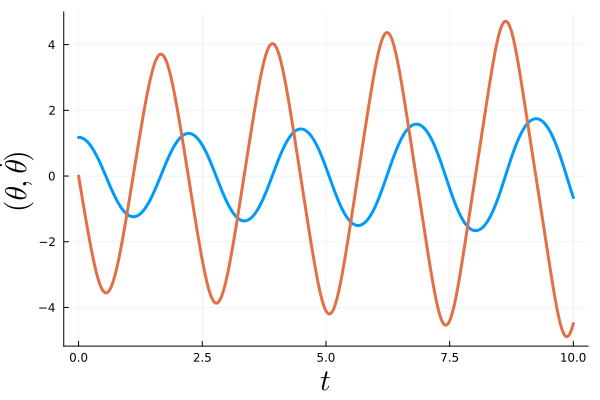
\includegraphics[width=\linewidth]{graphics/Chap09/PendulumSimulationChap09Eulerdt1eminus2.png}
        % \captionof{figure}{First Image Caption}
        % \label{fig:first_image}
    \end{minipage}
    \hfill
    \begin{minipage}{0.45\columnwidth}
        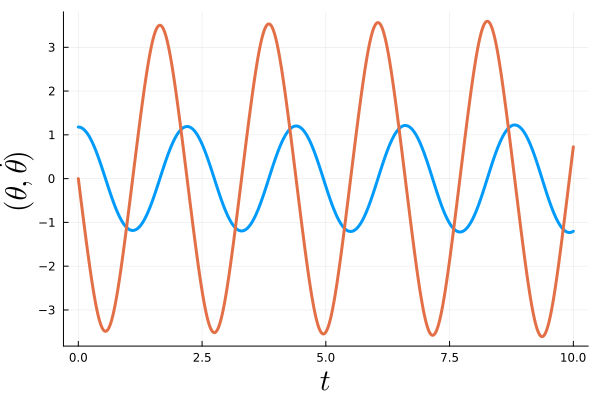
\includegraphics[width=\linewidth]{graphics/Chap09/PendulumSimulationChap09Eulerdt1eminus3.png}
        % \captionof{figure}{Second Image Caption}
        % \label{fig:second_image}
    \end{minipage}
\end{center}
 \bigskip

\item The 2-link robot arm stabilized in the upward equilibrium from Example~\ref{ex:StabilizeNonlinear2LinkRobotArmUpwardEquilibrium}.
 
\begin{lstlisting}[language=Julia,style=mystyle]
# Import useful packages
using Plots 
using LaTeXStrings
using LinearAlgebra # for the backslash command
gr()


# bring the model into the workspace for later use
include("dyn_mod_2LinkManipulator.jl") 

#Build a function to define the parameters of the model
function modelParameters()
    g = 9.81 # m/s^2
    L1 = 1 # m
    L2 = 0.7
    m1 = 15 # kg
    m2 = 10   
    return g, L1, L2, m1, m2
end

# Parameters for the Feedback controller

struct Params
    qe::Vector{Float64}      # equilibrium point
    K ::Matrix{Float64}      # LQR Feedback gain matrix
end
# Initialize the Params structure with specific values

K=[ 357.82  80.57  62.084   16.8291
  80.57  73.57  16.8291   6.92965]
qe = [pi/2, 0] # upward
params = Params(qe, K)


# define the ODE dx/dt = f(x,t)
#
# the parameters are passed via modelParameters() in the
# function dyn_mod_2LinkManipulator(q, dq)
#
function f(x,params,t)
    n = floor(Int, length(x) / 2) # In Julia n/2 is a Float64
    q = x[1:n]
    dq = x[n+1:end]
    K = params.K 
    qe = params.qe
    xe = [qe; 0*qe]
    tau = -K*(x-xe)
    model = dyn_mod_2LinkManipulator(q, dq)     
    dx1 = dq
    dx2 = (model.D) \ ( -model.C*dq-model.G+model.B*tau) # note the use of backslash
    dx=[dx1;dx2]
    return dx
end

# Set the initial condition as a vector
x0= [qe;0*qe] - [pi/4; pi/4; 0; 0]

# Set the time interval
T = (0.0, 8) 

# Euler's method
dt = 1e-2
N = floor(Int64,T[2]/dt)
x=zeros(4,N+1)
x[:,1]=x0
t=zeros(N+1)
t[1] = T[1]
for n=1:N
    t[n+1] = t[n]+dt
    x[:,n+1] = x[:,n] + dt*f(x[:,n],params,t[n])
end
#p1 = plot(t, x[1:2,:]', lw=3, guidefont = 20,  xlabel=L"t", ylabel=L"(q_1, q_2)", legend = ("q_1", "q_2"))
p1 = plot(t, x[1, :], lw=3, label="q1", guidefont=20, xlabel=L"t", ylabel=L"(q_1, q_2)",)
plot!(p1, t, x[2, :], lw=3, label="q2")
display(p1)
\end{lstlisting}
\textbf{Output} 
The feedback controller in this system was designed so that the eigenvalues of the closed-loop linearized model have negative real parts. In such cases, Euler tends to do quite well. Here, we see the first link converging to the upright position, $q_1 = \frac{\pi}{2}$, and the second link aligning itself with the first link, that is, $q_2=0$.

\begin{center}
    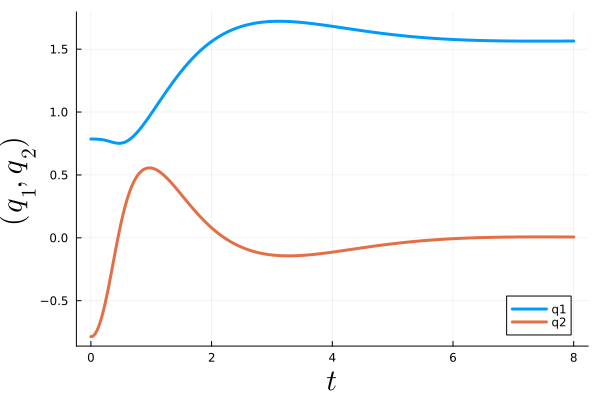
\includegraphics[width=0.6\columnwidth]{graphics/Chap09/2LinkManipulatorSimulationClosedLoopStatesEuler.png}
\end{center}

% \begin{lstlisting}[language=Julia,style=mystyle]

% \end{lstlisting}
% \textbf{Output} 
% \begin{verbatim}

% \end{verbatim}

\end{enumerate} 

\bigskip

\begin{factColor}{Derivation of Euler's Method or How to Never Forget It}{EulerMethodDerivation}

Consider an ODE $\dot{x} = f(x, t)$. Using a forward difference to approximate the derivative of $x(t)$ gives,
\begin{align*}
    \frac{x(t+ h) -x(t)}{h} &= f(x(t),t) \\
    & \Updownarrow \\
    x(t+h) - x(t) &= h \cdot f(x(t), t) \\
     & \Updownarrow \\
     x(t+h) & = x(t) +  h \cdot f(x(t), t) \\
          & \Updownarrow  ~~(\text{substituting in } t_{n+1} :=t_n+h)\\
     x(t_{n+1}) & = x(t_n) +  h \cdot f(x(t_n), t_n).
\end{align*}
The derivation is amazingly simple and easy to re-derive at a moment's notice when you need it most.
    
\end{factColor}

\section{Resonance in ODEs}



The collapse of the \href{https://en.wikipedia.org/wiki/Tacoma_Narrows_Bridge_(1940)}{Tacoma Narrows Bridge (1940)} (see also, the video \href{https://www.youtube.com/watch?v=j-zczJXSxnw}{Tacoma Narrows Bridge Collapse ``Gallopin' Gerti''}) in Washington State in 1940 serves as a stark reminder of the importance of considering dynamic effects in structural design. This event is often associated with the concept of resonance; however, the actual cause of the collapse is more accurately attributed to a phenomenon known as \textit{aeroelastic flutter}, which differs from resonance.

\textbf{Resonance} occurs when a system oscillates at its natural frequency due to external periodic driving forces at that same frequency. Initially, it was believed that the Tacoma Narrows Bridge collapsed due to resonance caused by wind. Further analysis, however, has shown that the situation was more complex.

\textbf{Aeroelastic Flutter} is a self-exciting and self-sustaining oscillation caused by the interaction between aerodynamic forces, elastic properties, and inertial forces of a structure. For the Tacoma Narrows Bridge, wind provided an external force that initiated oscillations in the bridge. The bridge's design—particularly its narrow, flexible, and lightweight construction—made it exceptionally vulnerable to these aeroelastic oscillations.


\bigskip

Below we consider a mass-spring system, with no damping. It has a natural frequency of oscillation, $\omega_n = \sqrt{k / m} $, where $k$ is the spring constant and $m$ is the mass. If one gives the system a tap, it will simply oscillate at its natural frequency. In the code below, we force the system with $\cos(\omega_0\, t)$, where $\omega_0$ is chosen as the natural frequency of the system. This creates a \textbf{resonance response} that grows like $t\, \cos(\omega_0\, t + \theta_0)$. The increasing amplitude with time will eventually cause any real-world system to reach its physical limits and break, similar to what aeroelastic flutter did to the \href{https://www.youtube.com/results?search_query=tacoma+narrows+bridge+collapse}{Tacoma Narrows Bridge}.

\bigskip

\begin{center}
    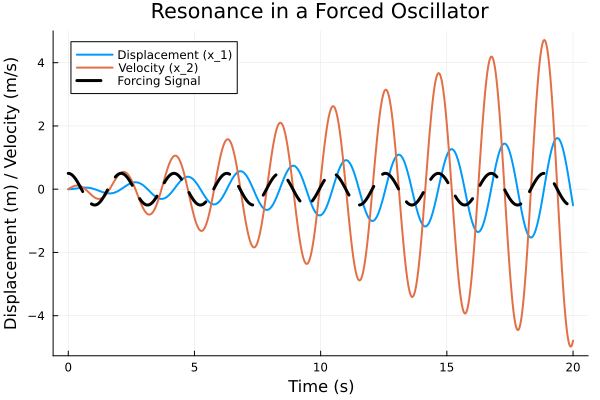
\includegraphics[width=0.6\columnwidth]{graphics/Chap09/ResonanceLinearSystem.png}
\end{center}


\begin{lstlisting}[language=Julia,style=mystyle]
using DifferentialEquations, Plots

# Constants
m = 1.0   # Mass (kg)
k = 9.0   # Spring constant (N/m)
F0 = 0.5  # Amplitude of the external force (N)
w_n = sqrt(k / m)  # Natural frequency (rad/s)
w = w_n   # Forcing frequency = Natural frequency for resonance

# ODE Definition
function forced_oscillator!(du, u, p, t)
    x, v = u
    du[1] = v
    du[2] = (F0*cos(w*t) - k*x) / m
end

# Initial conditions
u0 = [0.0, 0.0]  # Initial displacement and velocity
tspan = (0.0, 20.0)  # Time span

# Solve the ODE
prob = ODEProblem(forced_oscillator!, u0, tspan)
sol = solve(prob, Tsit5(), reltol=1e-8, abstol=1e-8)

# Create a finer time grid for interpolation
fine_t = range(tspan[1], tspan[2], length=10000) # Increased number of points for finer interpolation

# Interpolate the solution at the finer time grid
fine_x = [sol(t)[1] for t in fine_t]
fine_v = [sol(t)[2] for t in fine_t]

# Forcing signal
forcing_signal = F0*cos.(w.*fine_t)

# Plotting
p1 = plot(fine_t, fine_x, label="Displacement (x_1)", xlabel="Time (s)", ylabel="Displacement (m) / Velocity (m/s)", 
    title="Resonance in a Forced Oscillator", linewidth=2)
plot!(fine_t, fine_v, label="Velocity (x_2)", linewidth=2) # Smooth velocity curve
plot!(fine_t, forcing_signal, label="Forcing Signal", linestyle=:dash, color=:black, lw=3) # Forcing signal

# Display the plot
plot!(legend=:topleft)
\end{lstlisting}
\textbf{Output} 
See the above plot.

\bigskip
\textbf{(Optional Read:) Videos for Enhancing Your Understanding and Intuition:}
\begin{itemize}
    \item \href{https://youtu.be/dihQuwrf9yQ}{A better description of resonance} by Steve Mould. He illustrates wave patterns via the heights of flames! If you believe that fire makes anything better, then this video is for you. It's a bit slow initially, so you may want to jump ahead and then return to the beginning after you've seen the punchline. 

    \item \href{https://youtu.be/f4M-6tWtkoA}{Resonance and the Sounds of Music} by Walter Lewin. Very old-school set up by an absolute master with 1.64M subscribers. 

    \item \href{https://youtu.be/B_u3sGbpM8M}{Resonance Introduction using 9 Demonstrations} by Flipping Physics (so nerdy that the humor enhances understanding).
\end{itemize}
    


\section{(Optional Read:) More on Julia Packages for Solving ODEs and PDEs}

In Julia, the ecosystem for solving differential equations, including ordinary differential equations (ODEs) and partial differential equations (PDEs), is extensive and under continuous development. The primary effort that began under the umbrella of ``JuliaDiffE'' has since been integrated into a larger, more comprehensive initiative known as the \href{https://docs.sciml.ai/Overview/stable/}{SciML (Scientific Machine Learning)} ecosystem. This initiative aims to provide a cohesive suite of tools for scientific computing, which includes solving differential equations, machine learning in the context of scientific problems, and much more.

\begin{itemize}
  \item \textbf{For ODEs:}
  \begin{itemize}
    \item \textbf{DifferentialEquations.jl}: A flagship package within the SciML ecosystem offering a unified interface for solving a broad spectrum of differential equations, including ODEs, PDEs, stochastic differential equations (SDEs), and more. It is highly flexible and features many algorithms for solving ODEs.
    \item \textbf{OrdinaryDiffEq.jl}: A part of the DifferentialEquations.jl suite focused specifically on ODEs, providing a comprehensive array of solvers and analysis tools.
  \end{itemize}

  \item \textbf{For PDEs:}
  \begin{itemize}
    \item \textbf{DifferentialEquations.jl}: Also acts as the go-to tool for PDEs, offering methods to discretize and solve PDEs either directly or through conversion into ODEs or SDEs.
    \item \textbf{FEniCS.jl}: A Julia wrapper for the FEniCS project, an acclaimed open-source computing platform for solving PDEs using finite element methods, enabling Julia users to utilize FEniCS's potent PDE-solving capabilities.
    \item \textbf{Gridap.jl}: Provides a comprehensive toolkit for the simulation of PDEs using the finite element method (FEM), offering a powerful and adaptable framework for complex multiphysics simulations.
    \item \textbf{JuAFEM.jl}: Aimed at solving finite element method problems, focusing on a simple and intuitive interface for Julia users.
  \end{itemize}

  \item \textbf{Other Notable Packages:}
  \begin{itemize}
    \item \textbf{ModelingToolkit.jl}: Part of the SciML ecosystem designed to ease the modeling of scientific problems, including differential equations creation and manipulation, often used alongside DifferentialEquations.jl.
    \item \textbf{ParameterizedFunctions.jl}: Facilitates defining systems of differential equations with additional features like symbolic derivatives and parameter estimation, enhancing DifferentialEquations.jl's functionality.
    \item \textbf{PDEOperators.jl}: Offers tools for defining differential operators for PDE discretization, simplifying work with complex differential operators.
    \item \textbf{ApproxFun.jl}: Though not exclusively for differential equations, this package enables function approximation and can be used for solving differential equations.
  \end{itemize}
\end{itemize}

These packages are integral to a broader, highly integrated ecosystem that includes tools for optimization, machine learning, and beyond, allowing for advanced problem-solving approaches across various scientific fields. The Julia community actively develops and maintains these packages, ensuring regular updates and expansions to the ecosystem.



\section{(Optional Read:) Proofs Associated with the Chapter}
\label{sec:ODEproofs}


\begin{propColor}{Real Basis Vectors from Eigenvectors}{RealBasisVectorsFromEigenvectors}
Suppose that $A$ is a real $n \times n$ matrix. Then we know its eigenvalues and eigenvectors are either real or they occur in complex conjugate pairs. Let $\lambda_1, \ldots, \lambda_p, \lambda_1^\ast, \ldots, \lambda_p^\ast$ be the complex eigenvalues and let $\lambda_{2p+1}, \ldots, \lambda_n$ be the real eigenvalues, with a similar enumeration for the corresponding eigenvectors $\{v_1, \ldots, v_p, v_1^\ast, \ldots, v_p^\ast, v_{2p+1}, \ldots, v_n\}$. If the eigenvalues are distinct, that is $\lambda_i \neq \lambda_j$ for $i \neq j$, then the set of $n$ real vectors
$$ \{ v_{R1}, \ldots, v_{Rp},v_{I1}, \ldots, v_{Ip} , v_{2p+1}, \ldots, v_n \} $$
is linearly independent and forms a basis of $\real^n$. \\

Moreover, if $\lambda=\lambda_R + \im \lambda_I$ and $v = v_R + \im v_I$ are a complex eigenvalue and eigenvector, then
\begin{equation}
\label{eq:KeyToRealJordanForm}
    \begin{aligned}
        A v_R &= \lambda_R v_R -  \lambda_I v_I \\
        A v_I &= \lambda_I v_R +  \lambda_R v_I.
    \end{aligned}
\end{equation}
    
\end{propColor}

\textbf{Proof:} Chapter 2.7 of the ROB 501 textbook, \href{https://www.dropbox.com/scl/fi/5c656kxxzzwd1s6lgb6x7/ROB501_Textbook2022_03_21.pdf?rlkey=frdzx71ddh988vzvmd2izhd5y&dl=0}{Mathematics for Robotics}, establishes that the eigenvalues being distinct implies that the set of eigenvectors
$$ \{v_1, \ldots, v_p, v_1^\ast, \ldots, v_p^\ast, v_{2p+1}, \ldots, v_n\}$$
forms a basis of $(\cp^n, \cp)$. Hence, 
$$ \dim ~ \spanof{v_1, \ldots, v_p, v_1^\ast, \ldots, v_p^\ast, v_{2p+1}, \ldots, v_n} = n,$$
the dimension of $(\cp^n, \cp)$.\\

By the definition of the real and imaginary parts of vectors, for each $1 \le j \le p$, $v_j = v_{Rj} + \im v_{Ij}$ and $v_j^\ast = v_{Rj} - \im v_{Ij}$, and moreover, 
$ v_{Rj} = \frac{v_j + v_j^\ast}{2}$ and $v_{Ij} = \frac{v_j - v_j^\ast}{2 \im}$. Hence, 
$$ \spanof{v_j, v_j^\ast} =  \spanof{v_{Rj}, v_{Ij}}, $$
and 
$$\spanof{v_1, \ldots, v_p, v_1^\ast, \ldots, v_p^\ast, v_{2p+1}, \ldots, v_n} =  \{ v_{R1}, \ldots, v_{Rp},v_{I1}, \ldots, v_{Ip} , v_{2p+1}, \ldots, v_n \}.$$
It follows that
 $$\dim ~ \spanof{v_{R1}, \ldots, v_{Rp},v_{I1}, \ldots, v_{Ip} , v_{2p+1}, \ldots, v_n} = n,$$
 establishing the vectors are linearly independent in $(\cp^n, \cp)$, and hence also in $(\real^n, \real)$.\\

 To establish \eqref{eq:KeyToRealJordanForm}, we use 
 \begin{align*}
  A v =    A (v_R + \im v_I) & = (\lambda_R + \im \lambda_I) \cdot (v_R + \im v_I) = \lambda v\\
  A v^\ast=    A (v_R - \im v_I) & = (\lambda_R - \im \lambda_I) \cdot (v_R - \im v_I) = \lambda^\ast v^\ast.
 \end{align*}
 This gives 
  \begin{align*}
  Av_R =    A  \frac{v + v^\ast}{2} & = \lambda_R v_R -  \lambda_I v_I \\
  Av_I =    A  \frac{v - v^\ast}{2 \im} & = \lambda_I v_R +  \lambda_R v_I.
 \end{align*}
 An alternative proof is
   \begin{align*}
  Av_R =    {\rm real}(A v)& = {\rm real}\left( (\lambda_R + \im \lambda_I) \cdot (v_R + \im v_I) \right) = \lambda_R v_R -  \lambda_I v_I \\
  Av_I =    {\rm imag}(A v) & = {\rm imag}\left((\lambda_R + \im \lambda_I) \cdot (v_R + \im v_I)\right) = \lambda_I v_R +  \lambda_R v_I.
 \end{align*}

 
 \Qed

 \bigskip


\begin{propColor}{$e^{At} v_R$ and $e^{At} v_I$}{MatrixExponentialTimesvRandvI}
\begin{equation}
\label{eq:KeyToRealJordanFormMatrixExponential}
    \begin{aligned}
        e^{At} \, v_R &= e^{\lambda_R t }\, \cos(\lambda_I t) \, v_R -  e^{\lambda_R t} \, \sin(\lambda_I t) \,v_I \\
        e^{At} \, v_I &=  e^{\lambda_R t }\, \sin(\lambda_I t) \, v_R +  e^{\lambda_R t} \, \cos(\lambda_I t) \,v_I.
    \end{aligned}
\end{equation}
    
\end{propColor}
\textbf{Proof:} As in Prop.~\ref{thm:RealBasisVectorsFromEigenvectors}, we write $\lambda = \lambda_R + \im \lambda_I$ and $v = v_R + \im v_I$. Then, 
\begin{align*}
     e^{At} \, v_R & = {\rm real}\left( e^{At}  \, v\right)  \\
     &= {\rm real}\left( e^{\lambda t}  \, v\right) \\
     &= {\rm real}\left( e^{\lambda_R t} \left( \cos(\lambda_I t) + \im  \sin(\lambda_I t)\right)  \, \left( v_R + \im v_I
 \right) \right) \\
 & = e^{\lambda_R t }\, \cos(\lambda_I t) \, v_R -  e^{\lambda_R t} \, \sin(\lambda_I t) \,v_I
\end{align*}
Similarly,
\begin{align*}
     e^{At} \, v_I & = {\rm imag}\left( e^{At}  \, v\right)  \\
     &= {\rm imag}\left( e^{\lambda t}  \, v\right) \\
     &= {\rm imag}\left( e^{\lambda_R t} \left( \cos(\lambda_I t) + \im  \sin(\lambda_I t)\right)  \, \left( v_R + \im v_I
 \right) \right) \\
 & = e^{\lambda_R t }\, \sin(\lambda_I t) \, v_R +  e^{\lambda_R t} \, \cos(\lambda_I t) \,v_I
\end{align*}


\Qed
 

 \bigskip

 From Prop.~\ref{thm:LinearizedRobotEquations} Linearization of the Robot Equations, we have that the linearized model about any equilibrium point has the form
\begin{equation}
    \label{eq:RobotEqnLinearizedSecondOrderV03}
  \left[ \begin{array}{c} \delta \dot{x}_1 \\ \delta  \dot{x}_2 \end{array} \right] = \left[ \begin{array}{cc} 0_n & I_n \\ A_{21} & 0_n \end{array} \right] \left[ \begin{array}{c} \delta {x}_1 \\ \delta {x}_2 \end{array} \right].
\end{equation}

\bigskip

\begin{propColor}{Eigen-Facts about the Robot Equations}{EigenFactsRobotEquations}
Suppose the matrices \( A \) and \( B \) are invertible and that matrix \( C \) is defined as
\[ C = \begin{bmatrix} 0 & B \\ A & 0 \end{bmatrix}. \]
Then, 
\[ \det(C - \lambda I) = \det\begin{bmatrix} -\lambda I & B \\ A & -\lambda I \end{bmatrix} = \det(\lambda^2 I - AB). \]
Therefore, the eigenvalues of \( C \) are the square roots of the eigenvalues of \( AB \). So, they depend on the eigenvalues of \( AB \) rather than the individual eigenvalues of the matrices \( A \) and \( B \).\\

\textbf{Note:} If $AB$ has a negative real eigenvalue, then $C$ will have a pair of purely imaginary eigenvalues.  If $AB$ has a positive real eigenvalue, then $C$ will have both a positive and negative eigenvalue. If $AB$ has a pair of complex conjugate eigenvalues, then $C$ will have two complex conjugate pairs of eigenvalues.
\end{propColor}

\textbf{Proof:} Based on \href{https://math.stackexchange.com/questions/262563/eigenvalues-of-block-matrices-with-zero-diagonal-blocks}{Eigenvalues of block matrices with zero diagonal blocks}. Given two vectors \( u, v \in \mathbb{R}^n \), let \( w = \begin{bmatrix} u \\ v \end{bmatrix} \in \mathbb{R}^{2n} \) be the vector whose first \( n \) components are those of \( u \) and whose last \( n \) are those of \( v \). The matrix-vector product \( C \cdot w \) gives
\[ \begin{bmatrix} 0 & B \\ A & 0 \end{bmatrix} \begin{bmatrix} u \\ v \end{bmatrix} = \begin{bmatrix} Av \\ Bu \end{bmatrix}. \]
Therefore, solving \( Cw = \lambda w \) reduces to solving the following two matrix equations,
\[ \begin{cases} Av = \lambda u \\ Bu = \lambda v. \end{cases} \]
Since \( A \) and \( B \) are invertible, it follows that \( v = \lambda A^{-1}u \) and \( u = \lambda B^{-1}v \):
\[ \begin{cases} Av = \lambda \cdot \lambda B^{-1}v \\ Bu = \lambda \cdot \lambda A^{-1}u \end{cases} \rightarrow \begin{cases} BAv = \lambda^2 v \\ ABu = \lambda^2 u \end{cases} \]
We conclude that \( \lambda \in \mathbb{C} \) is an eigenvalue of \( C \) if, and only if, \( \lambda^2 \) is an eigenvalue of \( AB \) (or \( BA \), since they have the same eigenvalues).

\Qed


% \bigskip

% \begin{lstlisting}[language=Julia,style=mystyle]

% \end{lstlisting}
% \textbf{Output} 
% \begin{verbatim}

% \end{verbatim}

\bigskip

\begin{tcolorbox}[title=\textcolor{black}{Proof of Prop.~\ref{thm:PropertiesComplexExponentials} (Properties of Complex Exponentials)}, sharp corners, colback=green!30, colframe=green!80!blue, breakable, fonttitle=\bfseries]

Complex exponentials are fundamental in various fields of mathematics, engineering, and physics. Below are some of the key properties of complex exponentials, for $a, \omega \in \real$ and
$z:= a + \im \omega \in \cp$:

\begin{enumerate}
\renewcommand{\labelenumi}{(\alph{enumi})}
\setlength{\itemsep}{.2cm}
   
    \item \textbf{Periodicity:} The function $e^{\im \omega t}$ is periodic with period $T = \frac{2\pi}{|\omega|}$, for $\omega \neq 0$.

    \item \textbf{Multiplicative Property:} For any two complex numbers $z_1 = a_1 + \im \omega_1$ and $z_2 = a_2 + \im \omega_2$, the exponential function satisfies $e^{z_1\, t}\cdot e^{z_2 \, t} = e^{\left(z_1 + z_2\right)\, t}$.

    \item \textbf{Inverse:} The inverse of $e^{zt}$ is given by $e^{-zt}$.

    \item \textbf{Differentiation and Integration:} The derivative and antiderivative of $e^{zt}$ with respect to $t$ are: 
    \begin{itemize}
        \item $\frac{d}{dt}e^{zt} = ze^{zt}$ and 

        \item for $z \neq 0$, $\int e^{zt} dt = \frac{1}{z}e^{zt} + C$, where $C$ is the constant of integration.

    \end{itemize}
    \item \textbf{Conjugation:} The complex conjugate of $e^{\left(a + \im \omega \right)t}$ is $e^{\left(a - \im \omega \right)t}$.

    \item \textbf{Magnitude:} The magnitude of $e^{\left(a+ \im \omega \right)t}$ is $|e^{\left(a+ \im \omega \right)\, t}| = e^{at}$, which exhibits exponential growth or decay based on the sign of the real part,  $a$.
\end{enumerate}

  
\end{tcolorbox}
\textbf{Proof:}

\begin{enumerate}
\renewcommand{\labelenumi}{(\alph{enumi})}
\setlength{\itemsep}{1cm}
   
    \item \textbf{Periodicity:} By Euler's formula,  $e^{\im \omega t} = \cos(\omega t) + \im \sin(\omega t)$.  Because $ \cos(\omega (t +  \frac{2\pi}{|\omega|} )) = \cos(\omega t +  \sign(\omega){2\pi}) = \cos(\omega t)$ and $ \sin(\omega (t +  \frac{2\pi}{|\omega|} )) = \sin(\omega t +  \sign(\omega){2\pi}) = \sin(\omega t)$, it follows that  $e^{\im \omega (t + \frac{2\pi}{|\omega|})}  = e^{\im \omega t}$, proving periodicity with period  $\frac{2\pi}{|\omega|}$.

    \item \textbf{Multiplicative Property:} Let $z_1 = a_1 + \im \omega_1$ and $z_2 = a_2 + \im \omega_2$. Then
    \begin{align*}
        e^{z_1 t} & = e^{a_1 t} \cos(\omega_1 t) + \im  e^{a_1 t} \sin(\omega_1 t) \\
         e^{z_2 t} & = e^{a_2 t} \cos(\omega_2t) + \im  e^{a_2 t} \sin(\omega_2 t).
    \end{align*}
    Therefore, 
       \begin{align*}
        e^{z_1 t} \cdot e^{z_2 t} & = \left(e^{a_1 t} \cos(\omega_1 t) + \im  e^{a_1 t} \sin(\omega_1 t) \right) \cdot \left( e^{a_2 t} \cos(\omega_2t) + \im  e^{a_2 t} \sin(\omega_2 t) \right)  \\
        &= e^{a_1 t} \cdot e^{a_2 t} \left( \cos(\omega_1 t) + \im  \sin(\omega_1 t) \right) \cdot \left(\cos(\omega_2t) + \im  \sin(\omega_2 t) \right) \\
        &=  e^{a_1 t} \cdot e^{a_2 t} \left( \cos(\omega_1 t) \cos(\omega_2t) - \sin(\omega_1 t) \sin(\omega_2 t) \right) + \im e^{a_1 t} \cdot e^{a_2 t} \left( \cos(\omega_1 t) \sin(\omega_2t) + \sin(\omega_1 t) \cos(\omega_2 t) \right) \\
        &= e^{a_1 t} \cdot e^{a_2 t} \cos( (\omega_1 +\omega_2)t)  + \im e^{a_1 t} \cdot e^{a_2 t} \sin( (\omega_1 +\omega_2)t) \\
        &= e^{(a_1+a_2) t + (\omega_1 + \omega_2)t} \\
        &= e^{(z_1 + z_2)t}.
    \end{align*}

    \item \textbf{Inverse:} From (b), $e^{zt} \cdot e^{-zt} = e^{(z - z)t} = e^0 = 1$, and hence, $e^{-zt}$ is the multiplicative inverse of $e^{zt}$.

    \item \textbf{Differentiation and Integration:} The most important observation is that by using Euler's formula, we are only differentiating or integrating real functions.\\
    
    Suppose $z = a + \im \omega$, and write $e^{zt} = e^{at}\left( \cos(\omega t) + \im \sin(\omega t) \right) = e^{at} \cos(\omega t) + \im e^{at} \sin(\omega t) $. 
    \begin{itemize}
        \item By the product rule and chain rule,
        \begin{align*}
            \frac{d}{dt}e^{zt} &= \frac{d}{dt} \left(  e^{at} \cos(\omega t) \right) + \im  \frac{d}{dt} \left(  e^{at} \sin(\omega t) \right) \\
            & =  \left(  a \, e^{at} \cos(\omega t) - \omega  e^{at} \sin(\omega t) \right) + \im  \left(  a \,  e^{at} \sin(\omega t) + \omega e^{at} \cos(\omega t) \right) \\
            &= a \, e^{at}\left( \cos(\omega t) + \im \sin(\omega t) \right) + \im \omega \, e^{at}\left( \cos(\omega t) + \im \sin(\omega t) \right) \\
            &= (a + \im \omega) \cdot e^{at}\left( \cos(\omega t) + \im \sin(\omega t) \right) \\
            & = z e^{z t}.
        \end{align*} 

        \item We assume $z \neq 0$.  $\int e^{zt} dt = \int e^{at} \cos(\omega t) \, dt + \im \int e^{at} \sin(\omega t) \, dt$. We note that if one of $a$ or $\omega$ is equal to zero, then the two integrals are trivial to evaluate; we leave this case to the learner and assume, therefore, that both $a$ and $\omega$ are non-zero. Each of the two integrals requires two applications of integration by parts! We show all the steps for the first integral. \\

The integration by parts formula is given by,
\[
\int u dv = uv - \int v du.
\]

We set \(u = \cos(\omega t)\) and \(dv = e^{at} dt\) and compute
\begin{itemize}
    \item[1)]  \(du = -\omega \sin(\omega t) dt\), and
    \item[2)]  \(v = \int e^{at} dt = \frac{1}{a} e^{at}\), given \(a \neq 0\).
\end{itemize}


Using the integration by parts formula, we have,
\begin{align*}
    \int e^{at} \cos(\omega t) \, dt & = uv - \int v  \, du \\
    &= \left(\cos(\omega t) \cdot \frac{1}{a} e^{at}\right) - \int \left(\frac{1}{a} e^{at}\right) (-\omega \sin(\omega t))  \, dt \\
    &= \frac{1}{a} e^{at} \cos(\omega t) + \frac{\omega}{a} \int e^{at} \sin(\omega t)  \, dt.
\end{align*}


The second integral \(\int e^{at} \sin(\omega t)  \, dt\) can be solved similarly by integration by parts. Let's set \(u = \sin(\omega t)\) and \(dv = e^{at} dt\), then,
\begin{itemize}
    \item[3)] \(du = \omega \cos(\omega t) dt\), and 
    \item[4)] \(v = \frac{1}{a} e^{at}\).
\end{itemize}

Applying integration by parts again, we have,
\[
\int e^{at} \sin(\omega t) dt = \frac{1}{a} e^{at} \sin(\omega t) - \frac{\omega}{a} \int e^{at} \cos(\omega t)  \, dt,
\]
where we recognize $\int e^{at} \cos(\omega t) dt$ as the original integral.\\

\textbf{Solving for the Original Integral:} Let \(I = \int e^{at} \cos(\omega t)  \, dt\). From the steps above, we have,
\begin{align*}
I &= \frac{1}{a} e^{at} \cos(\omega t) + \frac{\omega}{a} \left( \frac{1}{a} e^{at} \sin(\omega t) - \frac{\omega}{a} I \right) \\
    &=  \frac{1}{a} e^{at} \cos(\omega t) + \frac{\omega}{a^2} e^{at} \sin(\omega t) - \frac{\omega^2}{a^2} I.
\end{align*}


Solving for \(I\), we find,
\begin{align*}
I + \frac{\omega^2}{a^2} I & = \frac{1}{a} e^{at} \cos(\omega t) + \frac{\omega}{a^2} e^{at} \sin(\omega t) \\
&\Downarrow \\
I \left(1 + \frac{\omega^2}{a^2}\right) & = \frac{e^{at}}{a} \cos(\omega t) + \frac{\omega}{a^2} e^{at} \sin(\omega t) \\
&\Downarrow \\
I& = \frac{e^{at}}{a + \frac{\omega^2}{a}} \left(\cos(\omega t) + \frac{\omega}{a} \sin(\omega t)\right) \\
&\Downarrow \\
I &= \frac{a e^{at}}{a^2 + \omega^2} \cos(\omega t) + \frac{\omega e^{at}}{a^2 + \omega^2} \sin(\omega t).
\end{align*}

Therefore, the antiderivative of \(e^{at} \cos(\omega t)\) is,
\[
\int e^{at} \cos(\omega t) dt = \frac{a e^{at}}{a^2 + \omega^2} \cos(\omega t) + \frac{\omega e^{at}}{a^2 + \omega^2} \sin(\omega t) + C,
\]
where \(C\) is the constant of integration.\\

\textbf{In a similar manner}, the antiderivative of \(e^{at} \sin(\omega t)\) is given by,
\[
\int e^{at} \sin(\omega t) \, dt = \frac{e^{at}}{a^2 + \omega^2} \left(  a \sin(\omega t)  - \omega \cos(\omega t) \right) + C,
\]
where \(C\) is the constant of integration.\\

\textbf{Now, we must combine the two antiderivatives to obtain the antiderivative for the original function.} \\

For the function \(f(t) = e^{at} \cos(\omega t) + \im e^{at} \sin(\omega t)\), the antiderivative is the sum of the two antiderivatives computed above. Thus,
\begin{align*}
\int f(t) \, dt & = \int e^{at} \cos(\omega t) \, dt +  \im  \int   e^{at} \sin(\omega t)\,  dt \\
    &= \frac{e^{at}}{a^2 + \omega^2} \left(a \cos(\omega t) + \omega \sin(\omega t)\right) + \im \frac{ e^{at}}{a^2 + \omega^2} \left(a \sin(\omega t) - \omega \cos(\omega t)  \right) + C \\
    & =\frac{e^{at}}{a^2 + \omega^2} \, a \, (\cos(\omega t) + \im \sin(\omega t)) -  \im \frac{e^{at}}{a^2 + \omega^2} \, \omega \, (\cos(\omega t) + \im \sin(\omega t)) + C \\
& = \frac{e^{at}}{a^2 + \omega^2} (a - \im \omega) (\cos(\omega t) + \im \sin(\omega t)) + C~~(\text{after combining like terms}).
\end{align*}
Recalling Euler's formula, \(e^{\im \omega t} = \cos(\omega t) +  \im \sin(\omega t)\). Substituting this into our expression gives,
\[
\int f(t) \, dt = \frac{e^{at}}{a^2 + \omega^2} (a - \im  \omega) e^{\im \omega t} + C.
\]

Noticing that \(a^2 + \omega^2 = (a + \im  \omega) (a - \im  \omega)\), \(a + \im  \omega = z\), and $e^{zt} = e^{at} \cdot e^{\im \omega t}$, we can rewrite the antiderivative as,
\[
\int f(t) \, dt = \frac{e^{at} \cdot  e^{\im \omega t} \cdot (a - \im  \omega)}{(a + \im \omega)(a - \im \omega)}  + C = \frac{1}{z} e^{zt} + C,
\]
when \(z\) is not zero.
\end{itemize}

  
    \item \textbf{Conjugation:}  Because $e^{\left(a + \im \omega \right)t} = e^{at} \left( \cos(\omega t) + \im \sin(\omega t) \right)$, the  complex conjugate of $e^{\left(a + \im \omega \right)t}$ is  $e^{at} \left( \cos(\omega t)-\im \sin(\omega t) \right) =e^{at} \left( \cos(-\omega t)+\im \sin(-\omega t) \right) = e^{\left(a - \im \omega \right)t}$.

    \item \textbf{Magnitude:} The magnitude of $e^{\left(a + \im \omega \right)t} = e^{at} \left( \cos(\omega t) + \im \sin(\omega t) \right)$ is 
    $$| e^{at} \cos(\omega t) + \im e^{at} \sin(\omega t)| = \sqrt{ \left( e^{at} \cos(\omega t) \right)^2 + \left( e^{at} \sin(\omega t) \right)^2} = \sqrt{\left( e^{at} \right)^2 \cdot \left(\cos^2(\omega t) + \sin^2(\omega t) \right)} = e^{at}.$$
\end{enumerate}
\Qed


\bigskip
\begin{tcolorbox}[title=\textcolor{black}{Proof of Prop.~\ref{thm:ExpStabilityLinearSystems} (Exponential Stability of Linear Systems of ODEs)}, sharp corners, colback=green!30, colframe=green!80!blue, breakable, fonttitle=\bfseries]

Let $A$ be a real $n \times n$ matrix with eigenvalues $\lambda_1, \lambda_2, \ldots, \lambda_n$, and consider the linear system of ODEs,
$$\dot{x} = Ax.$$
If ${\rm real}(\lambda_i)< 0$ for $1 \le i \le n$ (aka, the real parts of all eigenvalues are negative), then the \textbf{origin} is globally exponentially stable.  
\end{tcolorbox}
\textbf{Proof:} We give the proof for the case of distinct eigenvalues.  By Prop.~\ref{thm:RealBasisVectorsFromEigenvectors}, set of $n$ real vectors
$$ \{ v_{R1}, \ldots,  v_{Rp},v_{I1}, \ldots,  v_{Ip} , v_{2p+1}, \ldots, v_n \} $$
is linearly independent and forms a basis of $\real^n$. Hence, an arbitrary $x_0 \in \real^n$ can be written as a linear combination
$$x_0 = \sum_{j=1}^p \left(\alpha_j  v_{Rj} + \beta_j v_{Ij} \right)+ \sum_{j=2p+1}^n \gamma_j v_j.$$

Next, applying Prop.~\ref{thm:MatrixExponentialTimesvRandvI}, we have
\begin{align*}
    e^{At}\, x_0 &= \sum_{j=1}^p \left(\alpha_j e^{At}\,  v_{Rj} + \beta_j e^{At}\, v_{Ij} \right)+ \sum_{j=2p+1}^n \gamma_j e^{At}\, v_j \\
    &=  \sum_{j=1}^p \left(\alpha_j e^{At}\,  v_{Rj} + \beta_j e^{At}\, v_{Ij} \right)+ \sum_{j=2p+1}^n \gamma_j e^{At}\, v_j \\
    &= \sum_{j=1}^p \left(\alpha_j \left( e^{\lambda_{Rj} t }\, \cos(\lambda_{Ij} t) \, v_{Rj}  -  e^{\lambda_{Rj}  t} \, \sin(\lambda_{Ij} t) \,v_{Ij}  \right) + \beta_j \left( e^{\lambda_{Rj}  t }\, \sin(\lambda_{Ij} t) \, v_{Rj}  +  e^{\lambda_{Rj}  t} \, \cos(\lambda_{Ij} t) \,v_{Ij} \right) \right)+ \sum_{j=2p+1}^n \gamma_j e^{\lambda_j\, t}\, v_j \\
    &= \sum_{j=1}^p e^{\lambda_{Rj} t } \left( \alpha_j \left( \cos(\lambda_{Ij} t) \, v_{Rj} - \sin(\lambda_{Ij} t) \,v_{Ij}  \right) + \beta_j \left( \sin(\lambda_{Ij} t) \, v_{Rj} + \cos(\lambda_{Ij} t) \,v_{Ij} \right) \right) + \sum_{j=2p+1}^n \gamma_j e^{\lambda_j\, t}\, v_j.
\end{align*}

From this, we see that if all eigenvalues have negative real parts, then $x(t):=e^{At}\, x_0 \to 0_{n \times 1}$ as $t \to  \infty$, completing the proof. \\

\textbf{Note:} Suppose one of the eigenvalues has real part that is non-negative. Then by taking $x_0$ to be the (real part of) the corresponding eigenvector, we then have a solution that does not converge to zero. It will either oscillate, stay constant, or explode. 

\Qed





